% !TEX root = ../XJ_thesis.tex
%
\chapter{Real-world Noisy Image Dataset: A New Benchmark}
\label{sec:dataset}

\section{Introduction}

During the past decades, the statistical property of real-world noise has been studied for CCD and CMOS image sensors \cite{healey1994radiometric,tsin2001statistical,RENOIR2014,crosschannel2016,dnd2017}. There are mainly five major sources for real-world noise, including photon shot noise, fixed pattern noise, dark current, readout noise, and quantization noise, etc. The shot noise is one inevitable source of noise, which is induced by the stochastic arrival process of photons to the sensor. It can be modeled by a Possion process in which the number of photons arriving the sensor follows a Possion distribution. This type of noise is proportional to the mean intensity of the specific pixel and is not stationary across the whole image. The fixed pattern noise include pixel response non-uniformity (PRNU) noise and dark current non-uniformity (DCNU) noise. In PRNU noise, each pixel will have a slightly different output levels or responses for a fixed light level. The major cause of the PRNU noise is the loss of light and color mixture in the neighboring pixels. The DCNU noise comes from the electronics within the sensor chip, and it is generated due to thermal agitation, even thouth there is no light reaching the camera sensor. The readout noise and quantization noise come from the discretization of measured signals. The readout noise is generated during the process of Charge-to-voltage conversion, which is inheretantly not accurate. This inaccuracy also happens to generate the quantization noise, in which the readout values are quantizated to be an integer. The final pixel values are only discretization of the original raw pixel values. Other noise include CCD specific sources such as transfer efficiency, and CMOS specific sources such as column noise.

Different from the additive white Gaussian noise (AWGN), the real-world noise is signal dependent, and cannot be modeled by an explicit distribution. It becomes much more complex after being processed in the camera imaging pipelines. Hence, removing real-world noise from real-world noisy images is a more challenging task than its synthetic AWGN counterpart. Another issue about real-world image denoising is how to evaluate the quality of the denoised images. The image quality assessment by subjective evaluation would be time-consuming, since it needs huge number of subjectives to take part in the evaluation experiments. An alternative is to resort to the objective evaluation. However, since the noisy image with real-world noise has no corresponding ``ground truth'' image, the objective evaluation on the quality of denoised images is very hard. Another alternative is to resort to some existing blind image quality assessment (BIQA) methods \cite{bliinds,biqi}. However, these BIQA methods are only effective on the commonly tested datasets such as TID dataset \cite{tid2008} and LIVE IQA dataset \cite{LIVEIQA}, and will fail at the real-world noisy images, which have very different noise statistics when compared to the noise in the TID \cite{tid2008} and LIVE IQA \cite{LIVEIQA} datasets.

Recently, several works have been done to fill in the gap of missing corresponding ``ground truth'' image to the captured real-world noisy image. In \cite{crosschannel2016}, a dataset containing 11 scenes is constructed for analyzing the properties of real-world noise during the camera imaging pipeline. However, this dataset is limited in several aspects. It contains only printed pictures on the package of several products, having few real objects. Other problems include that the intensity transform does not model heteroscedastic noise, and low-frequency bias is not removed, etc. In \cite{RENOIR2014} and \cite{dnd2017}, the corresponding ``ground truth'' image of the captured real-world noisy image is captured with low ISO values (e.g., ISO=100), with other post-processing steps include linear intensity changes, spatial misalignment, and low-frequency residual correciton, etc. However, the ``ground truth'' images with low ISO values may have slightly different illuminations with the real-world noisy image captured under high ISO values (e.g., ISO=6,400). Besides, the post-processing steps may introduce human bias into the ``ground truth'' images. The work of \cite{EMVA1288} proposes a less tedious capture protocol similar to \cite{dnd2017}, where multiple exposures of a static scene are used to aggregate the measurements at every pixel site temporally. The works of \cite{noisemeasurement,moldovan2006denoising} propose to illuminate the sensor with approximately constant irradiation and subsequently aggregates intensity measurements spatially. This is repeated for different irradiation levels to capture the intensity dependence of the noise. In contrast, in \cite{dnd2017} the employed Tobit regression allows to estimate the parameters of the noise process by having access to just two images.

In this work, we construct a large dataset of real-world noisy images with reasonably obtained corresponding ``ground truth'' images. The basic idea is to capture the same and unchanged scene for many (e.g., 500) times and compute their mean image, which can be roughly taken as the ``ground truth'' image for the real-world noisy images. The rational of this strategy is that for each pixel, the noise is generated randomly larger or smaller than the true pixel value. Sampling the same pixel many times and computing the average value will approximate the truth pixel value and alleviate significantly the noise.

\section{Existing Datasets}

Currently, there are several work focus on benchmarking the denoising methods on real-world noisy images \cite{RENOIR2014,crosschannel2016,dnd2017}.

As far as we know, the RENOIR dataset \cite{RENOIR2014} is the first dataset on real-world noisy images with ``ground truth'' noise-free images. The cameras used in this dataset are Canon Rebel T3i, Canon S90, and Xiaomi T3i. The authors took photos of a static scene with different ISO values. However, the post-processing is less refined. Image pairs appear to exhibit spatial misalignment, the intensity transform does not model heteroscedastic noise, and low-frequency bias is not removed. In \cite{RENOIR2014}, experiments have been conducted to validate that ignoring these factors makes the dataset less usefull. It is often useful to measure the noise characteristics of a sensor at a certain ISO level. \cite{RENOIR2014} proposes to illuminate the sensor with approximately constant irradiation and subsequently aggregates intensity measurements spatially. This is repeated for different irradiation levels to capture the intensity dependence of the noise. \cite{RENOIR2014} also proposes a less tedious capture protocol, where multiple exposures of a static scene are used to aggregate the measurements at every pixel site temporally. The detailed description of this dataset is listed in Table \ref{tab6-1}.

\begin{table}[t!]
\caption{Cameras and camera settings for capturing the dataset \cite{RENOIR2014}.}
\label{tab6-1}
\begin{center}
\small
\renewcommand\arraystretch{1.2}
\begin{tabular*}{1\textwidth}{@{\extracolsep{\fill}}c|cc|cc|cc}
\hline
\multirow{2}{*}{Camera}
&
\multirow{2}{*}{Sensor size (mm)}
&
\multirow{2}{*}{\# Scene}
&
\multicolumn{2}{c|}{``Ground Truth''}
&
\multicolumn{2}{c}{Noisy Image}
\\
&
&
&
ISO
&
Time (s)
&
ISO
&
Time (s)
\\
\hline
Canon S90 & $7.4\times5.6$ & 40 & 100  & 3.2  & 640, 1k & Auto 
\\
\hline   
Canon T3i & $22.3\times14.9$ & 40 & 100 & Auto  & 3.2k, 6.4k & Auto
\\
\hline
Xiaomi Mi3 & $4.69\times3.52$ & 40 & 100  & Auto  & 1.6k, 3.2k & Auto
\\
\hline
\end{tabular*}
\end{center}
\end{table}

The second work along this direction is reported in \cite{crosschannel2016}, which involves 11 static scenes. The real-world noisy images and the corresponding ``ground truth'' images are collected. For each scene, 500 JPEG images are captured and the mean image of the 500 images is roughly taken as the ``ground truth'' image. Utilizing the mean of temporal images as ``ground truth'' image has also been employed in \cite{Liu2008,liupractical}, in which the authors did not construct a benchmark dataset. In the dataset of \cite{crosschannel2016}, the images are mostly with resolution of $7630\times4912$ and captured by Nikon D800 (ISO=1,600, 3,200, and 6,400), Nikon D600 (ISO=3,200), and Canon 5D Mark III (ISO=3,200). There are totally 15 cropped regions of size $512\times512$ provided for evaluating different denoising methods. The major problems of this dataset is that the captured images are almost printed scenes, which share similar nosie statistical property. The camera settings are also somewhat limited such as the ISO values. The detailed description of this dataset is listed in Table \ref{tab6-2}. 

\begin{table}[t!]
\caption{The detailed information of the cropped regions from the dataset \cite{crosschannel2016}.}
\label{tab6-2}
\begin{center}
\small
\renewcommand\arraystretch{1.2}
\begin{tabular*}{1\textwidth}{@{\extracolsep{\fill}}ccccc}
\hline
Camera
& 
ISO
&
\# Scene
&
JPEG
&
Image size
\\
\hline
Canon 5D Mark III & 3.2k  & 3  & Fine & $512\times512$
\\
\hline
Nikon D600 & 3.2k & 3  & Normal & $512\times512$
\\
\hline   
Nikon D800 & 1.6k, 3.2k, 6.4k & 3  & Normal & $512\times512$
\\
\hline
\end{tabular*}
\end{center}
\vspace{-4mm}
\end{table}

One recent benchmark is reported in \cite{dnd2017}. Different from the other two datasets, \cite{dnd2017} employs the Tobit regression which allows to estimate the parameters of the noise process by accessing just two images. In order to obviate the unrealistic setting by developing a methodology for benchmarking denoising techniques on real photographs, the authors in \cite{dnd2017} captured 50 different pairs of images with different ISO settings and shutter speed. The image captured with high ISO and shorter shutter speed is taken as the real-world noisy image, while the image captured with low ISO and longer shutter speed is roughly taken as the ``ground truth'' image. To derive better ``ground truth'', careful post-processing is designed in \cite{dnd2017}. The authors corrected spatial misalignment, coped with the inaccuracies in the exposure parameters through a linear intensity transform based on a novel heteroscedastic Tobit regression model, and removed residual low-frequency bias that stems from minor illumination changes, etc. The proposed dataset is called the Darmstadt Noise Dataset (DND) \cite{dnd2017}, in which the cameras used for capturing the dataset include Sony A7R, Olympus E-M10, Sony RX100 IV, and Huawei Nexus 6P. The authors of \cite{dnd2017} extracted the linear raw intensities from the captured images using the free software \textsl{Dcraw}, and then normalized the image intensities to the range of $[0, 1]$ by scaling with the black and white level. One interesting finding is that various recent techniques that perform well on synthetic noise are clearly outperformed by BM3D \cite{bm3d} on realistic photographs. This benchmark delineates realistic evaluation scenarios that deviate strongly from those commonly used in the scientific literature. The detailed description of this dataset is listed in Table \ref{tab6-3}.

\begin{table}[t!]
\caption{Cameras and camera settings for capturing the dataset \cite{dnd2017}.}

\label{tab6-3}
\begin{center}
\small
\renewcommand\arraystretch{1.2}
\begin{tabular*}{1\textwidth}{@{\extracolsep{\fill}}cccc}
\hline
Camera
&
\# Scene
&
Sensor size (mm)
&
ISO
\\
\hline
Sony A7R & 13  & $36\times24$  & 100-25.6k
\\
\hline
Olympus E-M10 & 13  & $17.3\times13$  & 200-25.6k 
\\
\hline   
Sony RX100 IV & 12 & $13.2\times8.8$  & 125-8k 
\\
\hline   
Huawei Nexus 6P & 12 & $6.17\times4.55$  & 100-6.4k 
\\
\hline
\end{tabular*}
\end{center}
\vspace{-4mm}
\end{table}


\section{The Proposed Dataset}

\subsection{Motivation}
As discussed previously, existing real-world noisy image datasets \cite{RENOIR2014,crosschannel2016,dnd2017} have several limitations in evaluating existing and future image denoising methods. These limitations include camera brands, camera settings, and captured scenes, etc.

\textbf{Camera Brands}: In the RENOIR dataset \cite{RENOIR2014}, the authors used two different camera brands, Canon (T3i and S90) and Xiaomi (Mi3), for image collection. In the dataset \cite{crosschannel2016}, the authors also used these two camera brands, i.e., the Canon (5D) and Nikon (D600 and D800), for image collection. In the DND dataset \cite{dnd2017}, the authors used three different cameras including Sony (A7R and RX100 IV), Olympus (E-M10), and Huawei (Nexus 6P).

\textbf{Camera Settings}: In the RENOIR dataset \cite{RENOIR2014}, the ``ground truth'' images are all captured by setting the ISO as 100. The ISO in noisy images are set as follows: for Xiaomi Mi3, the ISO is set as 1,600 or 3,200; for Canon S90, the ISO is set as 640 or 1,000; for Canon T3i, the ISO is set as 3,200 or 6,400. For all the cases except for the reference image of Canon S90, the shutter speed is set as automatic. For Canon S90, the shutter speed is set as 3.2 seconds. In the dataset \cite{crosschannel2016}, three different ISOs (e.g., 1,600, 3,200, and 6,400) are employed when capturing images with Nikon D800, while ISO=3,200 is utilized for Canon 5D and Nikon D600. The DND dataset \cite{dnd2017} contains ISOs of large range. The ranges of ISO are $100\sim25,600$ for Sony A7R, $200\sim25,600$ for Olympus E-M10, $125\sim8,000$ for Sony RX100 IV, and $100\sim6,400$ for Huawei Nexus 6P, respectively. 

\textbf{Captured Scenes}: The RENOIR dataset \cite{RENOIR2014} capture 40 scenes for each camera brand, and overall 120 scenes are included in the dataset. However, the noisy images and corresponding ``ground truth'' images in this dataset have distinct color difference, which is largely caused by different lighting conditions. The dataset \cite{crosschannel2016} contains only 11 indoor scenes, in which these scenes are overlapped by similar contents and objects. Though containing 50 different scenes, the ``ground truth'' images in the DND dataset \cite{dnd2017} are not accessible. This will limit the evaluation of the proposed denoising methods on visual quality.


\textbf{Discussion}. Among the above mentioned factors, the camera settings are very important when we capture the real-world noisy images, while the camera brands and captured scenes are relatively easy to improve. The camera settings include mainly ISO value, the shutter speed, and the aperture, etc. In general, the faster the shutter speed, the darker the captured images, when we fix the other settings, and vice versa. Similarly, the smaller the ISO value (or aperture), the darker the captured images, when we fix the other settings, and vice versa. 

In order to make the image less affected by the change of the environment (e.g., object motion, change of illumination, camera shake, etc.), the shutter speed should be set as faster as possible. The shutter speed of the Sony A7II camera is between 1/80,000 second to 30 seconds. Given suitable aperture and ISO, it is possible to capture images with normal illuminations when we set the shutter speed between 1/100 second and 1 second. The aperture could be set as any value as long as it is in the reasonable range. The aperture of the Sony camera is between F3.5 and F22. Setting the aperture between F3.5 and F15 can allow us to obtain images with normal illumination under the fixed ranges of shutter and ISO. In our capturing process, we fixed the shutter and aperture in a suitable range, and tuned the ISO values according to the given camera. In general, the noise level would be higher when the ISO is higher. We set the ISO values from a low value to a high value with fixed gap to more comprehensively evaluate the denoising methods.

To analyze how ISO, shutter speed, and aperture influence the content and illumination of the captured images, we perform some heuristic experiments with different camera settings. In Figure \ref{fig6-1}, we show some images captured with different camera settings. Comparing Figures \ref{fig6-1}(a) and \ref{fig6-1}(b) (or \ref{fig6-1}(g) and \ref{fig6-1}(i)), we can find that higher aperture results in darker illumination. Comparing Figures \ref{fig6-1}(b) and \ref{fig6-1}(c) (or \ref{fig6-1}(g) and \ref{fig6-1}(h)), we can find that longer shutter results in brighter illumination. Comparing Figrues \ref{fig6-1}(b), \ref{fig6-1}(d), \ref{fig6-1}(e), \ref{fig6-1}(f), and \ref{fig6-1}(g), we can find that the illumination becomes brighter when the ISO is higher. Besides, given fixed aperture and shutter, the images captured by the camera can avoid the over-exposure or under-exposure when the ISO is set between 400 and 3,200. When ISO=200, the captured images would have the problem of underexposure, while when ISO=6,400, the captured images would have the problem of over-exposure. However, this can be alleviated by changing the aperture and shutter and finally we can obtain images with normal illuminations.

Given fixed shutter speed and aperture, enhancing the camera sensitivity will generate stronger noise than lowering the shutter speed. In the construction of our dataset, we only changed the ISO values while fixing shutter and aperture with suitable values to ensure that the images will not suffer over-exposure or under-exposure. It is commonly accepted that the noise in images will become stronger when the scene is under darker light source.



\begin{figure}[t!]
    \centering
\subfigure{
\begin{minipage}[t]{0.32\textwidth}
\centering
\raisebox{-0.5cm}{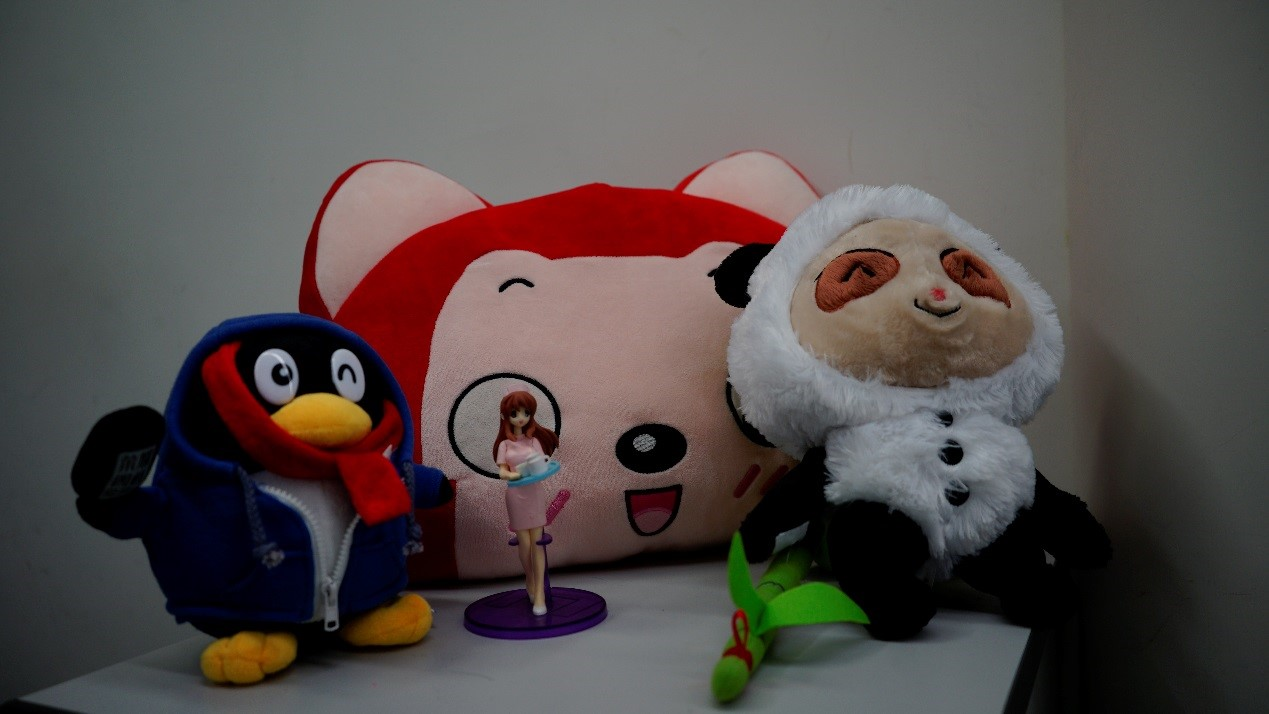
\includegraphics[width=1\textwidth]{images/dataset/200_3-5_1-60.jpg}}
{\footnotesize 200,3.5,1/60}
\end{minipage}
\begin{minipage}[t]{0.32\textwidth}
\centering
\raisebox{-0.5cm}{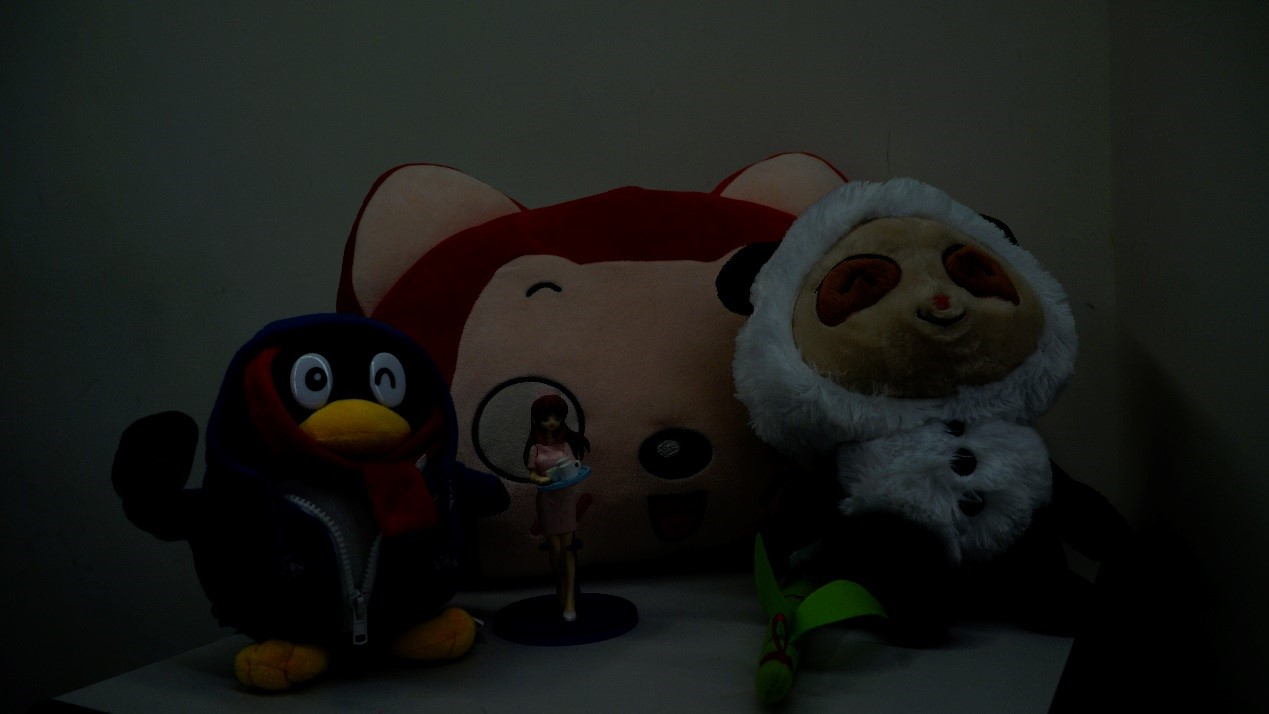
\includegraphics[width=1\textwidth]{images/dataset/200_6-7_1-60.jpg}}
{\footnotesize 200,6.7,1/60}
\end{minipage}
\begin{minipage}[t]{0.32\textwidth}
\centering
\raisebox{-0.5cm}{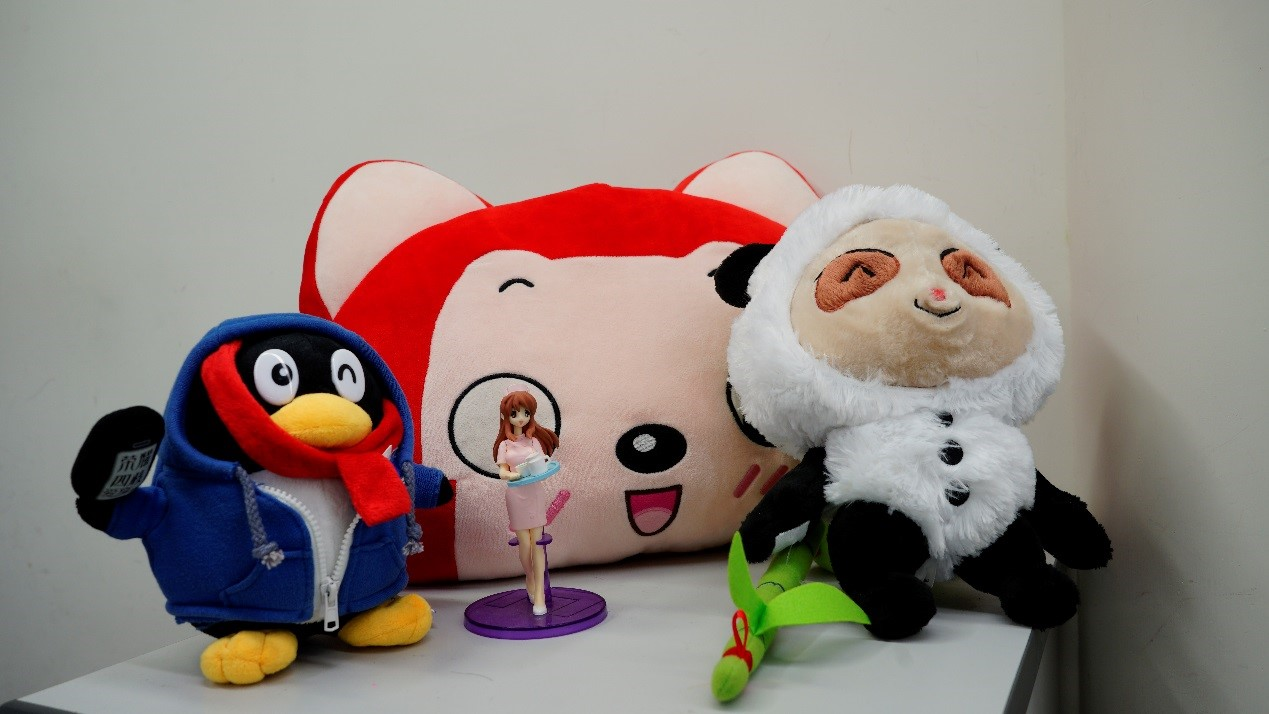
\includegraphics[width=1\textwidth]{images/dataset/200_6-7_1-8.jpg}}
{\footnotesize 200,6.7,1/8}
\end{minipage}
}\vspace{-3mm}
\subfigure{
\begin{minipage}[t]{0.32\textwidth}
\centering
\raisebox{-0.5cm}{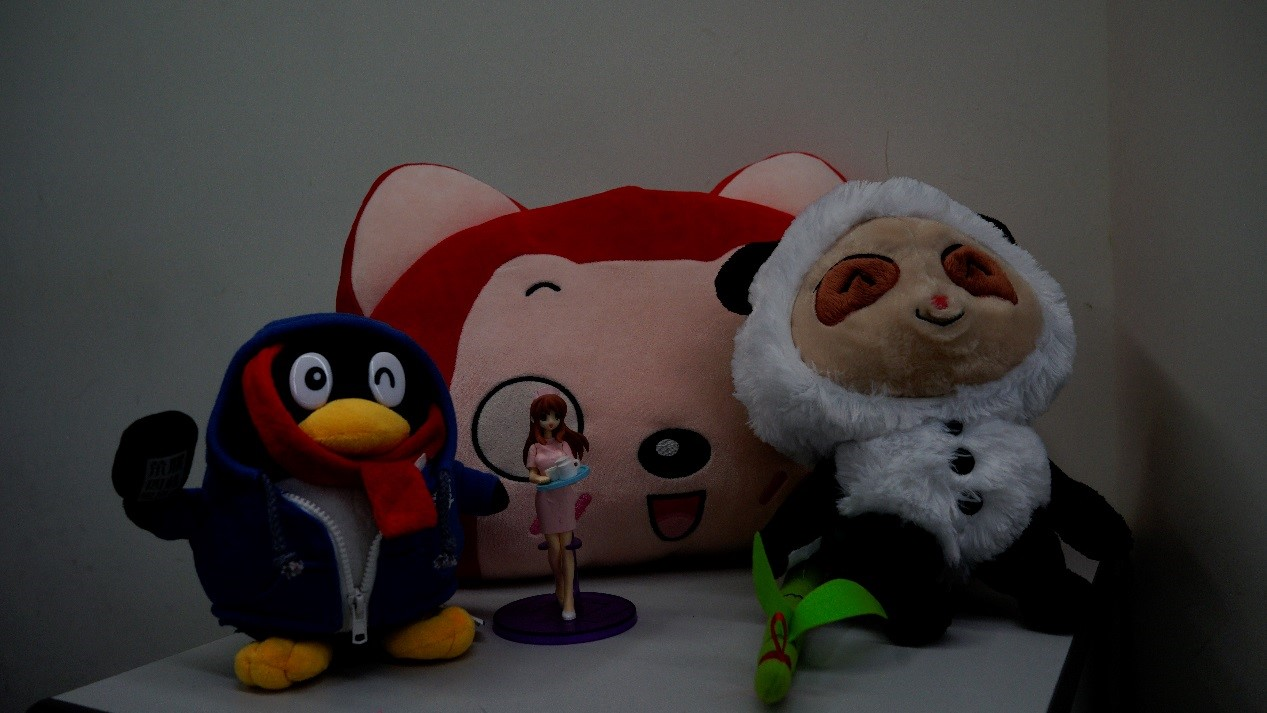
\includegraphics[width=1\textwidth]{images/dataset/400_6-7_1-60.jpg}}
{\footnotesize 400,6.7,1/60}
\end{minipage}
\begin{minipage}[t]{0.32\textwidth}
\centering
\raisebox{-0.5cm}{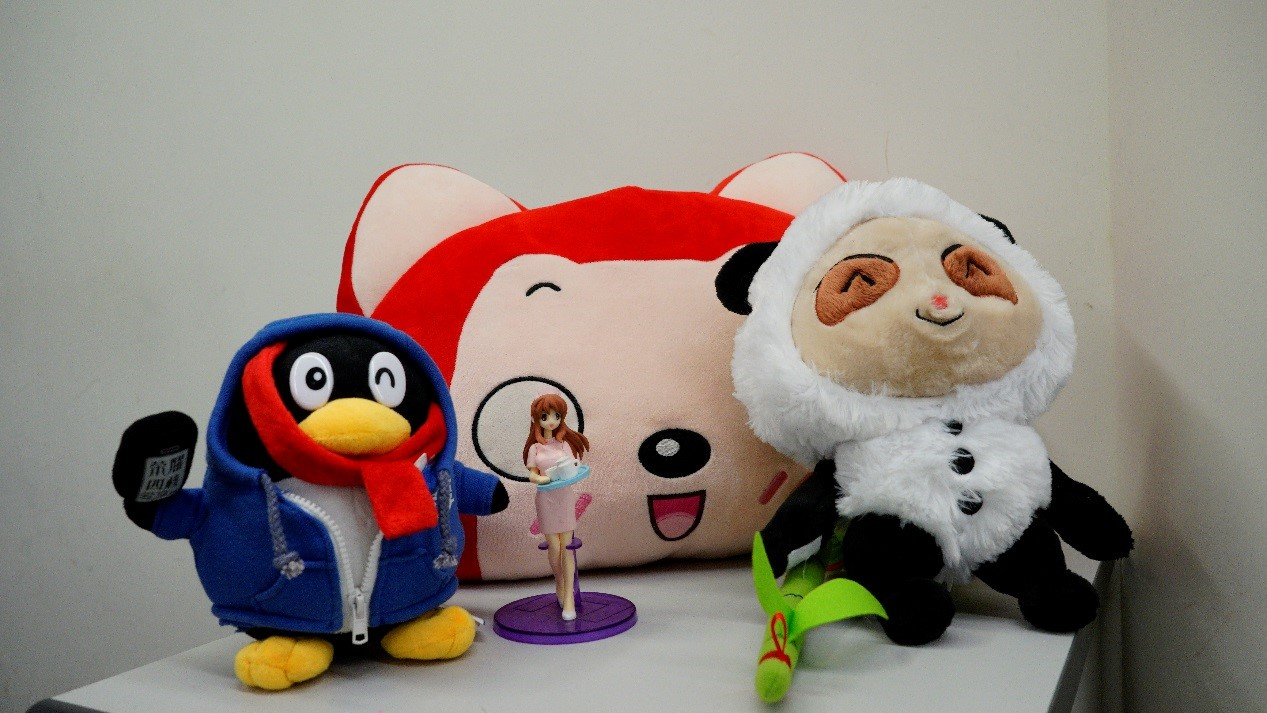
\includegraphics[width=1\textwidth]{images/dataset/1600_6-7_1-60.jpg}}
{\footnotesize 1600,6.7,1/60}
\end{minipage}
\begin{minipage}[t]{0.32\textwidth}
\centering
\raisebox{-0.5cm}{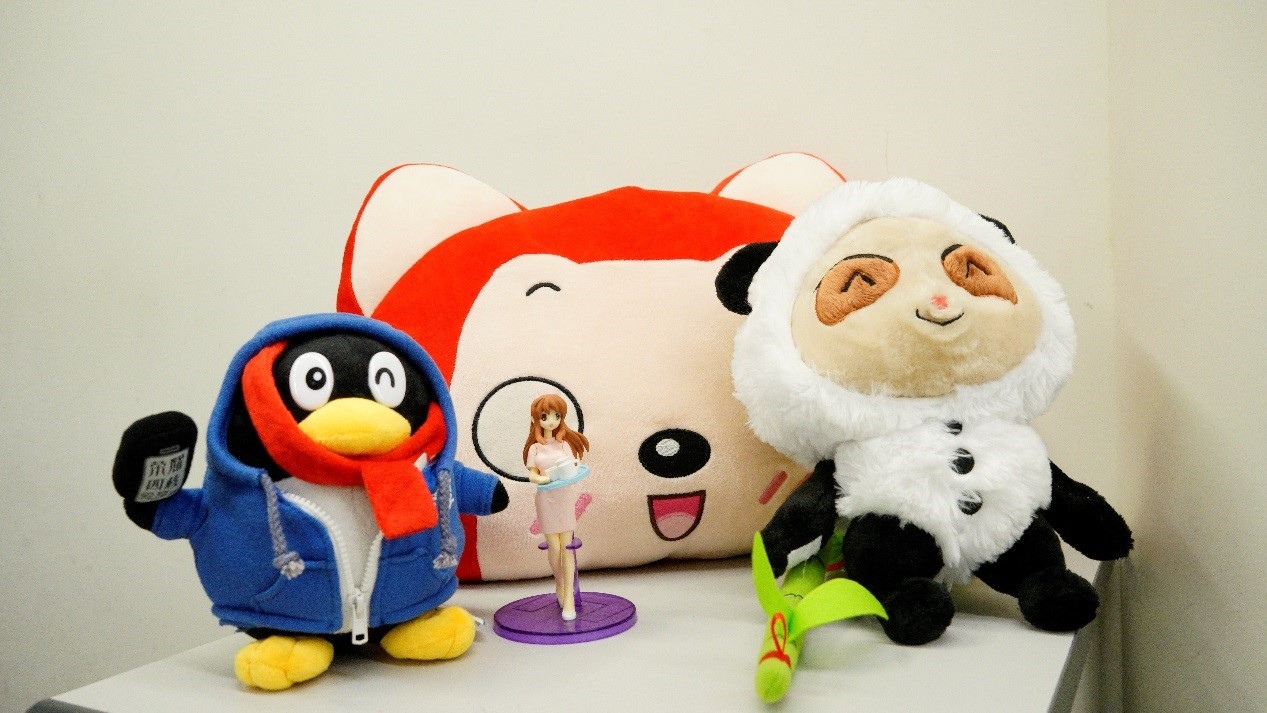
\includegraphics[width=1\textwidth]{images/dataset/3200_6-7_1-60.jpg}}
{\footnotesize 3200,6.7,1/60}
\end{minipage}
}\vspace{-3mm}
\subfigure{
\begin{minipage}[t]{0.32\textwidth}
\centering
\raisebox{-0.5cm}{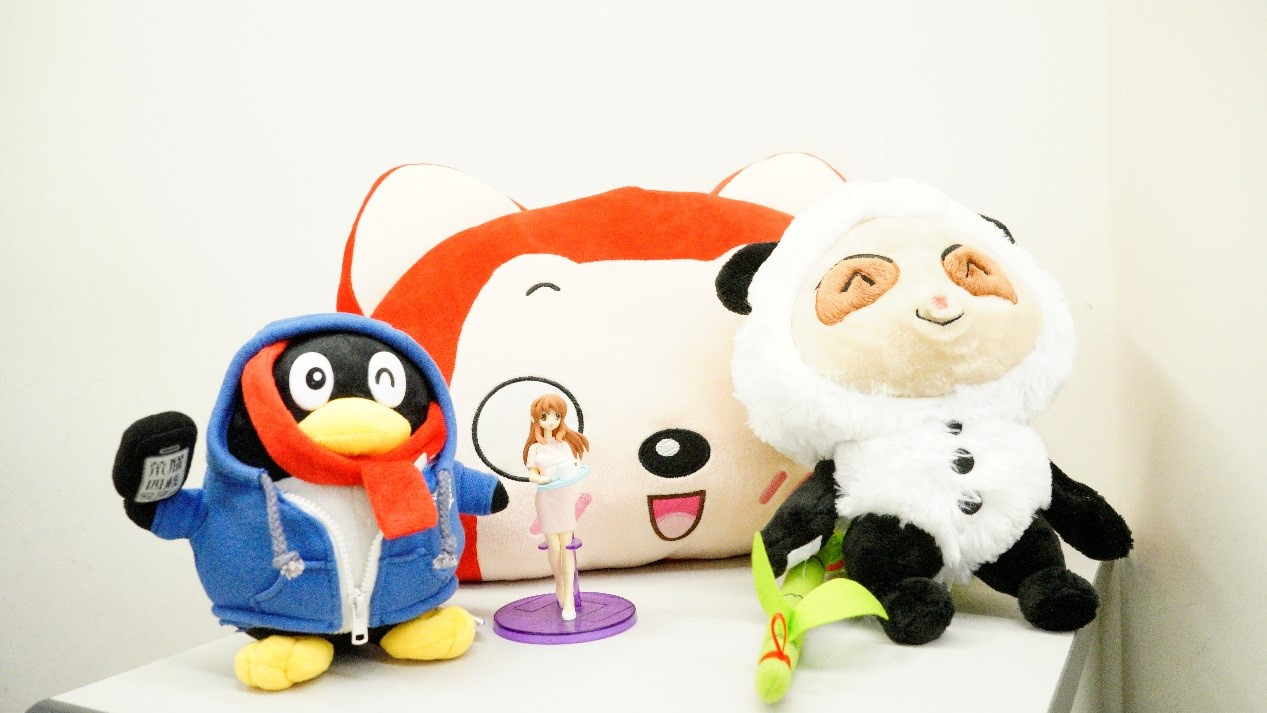
\includegraphics[width=1\textwidth]{images/dataset/6400_6-7_1-60.jpg}}
{\footnotesize 6400,6.7,1/60}
\end{minipage}
\begin{minipage}[t]{0.32\textwidth}
\centering
\raisebox{-0.5cm}{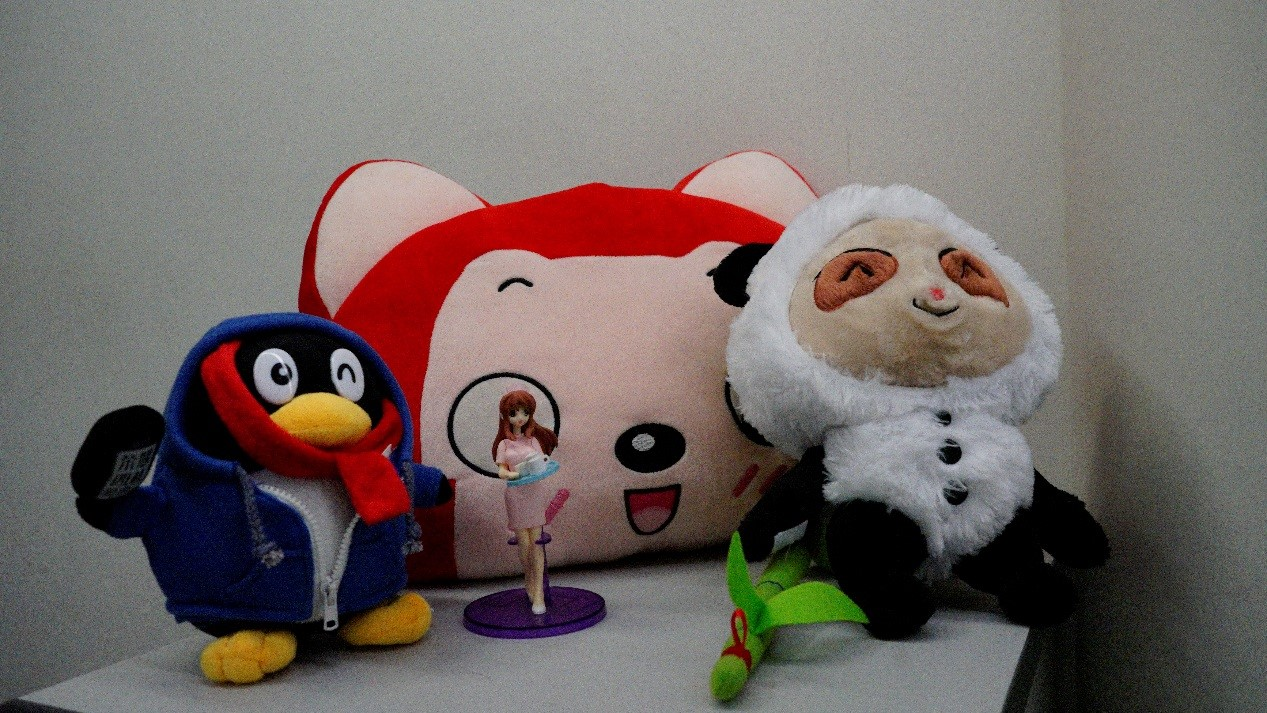
\includegraphics[width=1\textwidth]{images/dataset/6400_6-7_1-350.jpg}}
{\footnotesize 6400,6.7,1/350}
\end{minipage}
\begin{minipage}[t]{0.32\textwidth}
\centering
\raisebox{-0.5cm}{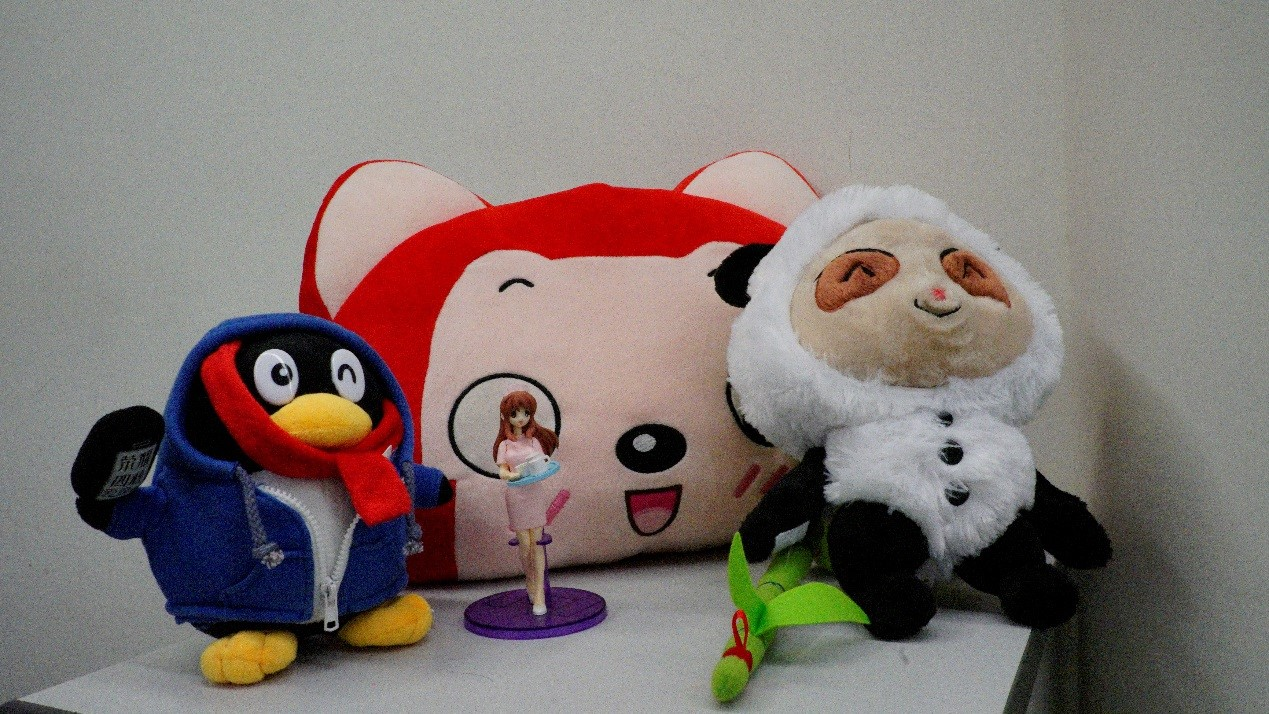
\includegraphics[width=1\textwidth]{images/dataset/6400_16_1-60.jpg}}
{\footnotesize 6400,16,1/60}
\end{minipage}
}\vspace{-3mm}
    \caption{Captured Images with the Sony A7 II camera under different (ISO, Shutter, Aperture) settings.}
    \label{fig6-1}
\end{figure}


\subsection{The Construction Process}

To alleviate the limitations of the previous datasets \cite{RENOIR2014,crosschannel2016,dnd2017}, we propose to construct a new dataset which could: 1) contain more camera brands; 2) contain more carefully designed camera settings; 3) capture more real-world scenes with realistic objects; 4) capture both the raw data and sRGB data for comparison analysis. The captured images are stored in raw data and JPEG format without compression. For each scene, we capture it for 500 times. Figure \ref{fig6-2} shows how we capture images of a static scens in indoor environment. The camera is fixed by a tripod. The capture is automatically done with shutter release. Hence, the misalignment problem can be nearly avoided in the accquisition process of 500 images for one scene. We capture images with different camera settings. The cameras are set based on the following rules. First, the shutter speed should be faster than the blink of the fluorescent lights, otherwise the flickering of the light will make the global illuminances of the captured images very different. Second, we set the shutter speed, the aperture, and the ISO value to ensure that the scenes are in a naturally lighting condition. Besides, since the digital single-lens reflex cameras (DSLRs) use mechanical shutter, the shutter speed of each shot is a little different. This small difference results in slightly different brightness of different shots. However, we ignore this small difference in our dataset, as that in \cite{crosschannel2016}.

\begin{figure}[t!]
    \centering
\subfigure{
\begin{minipage}[t]{0.4\textwidth}
\centering
\raisebox{-0.5cm}{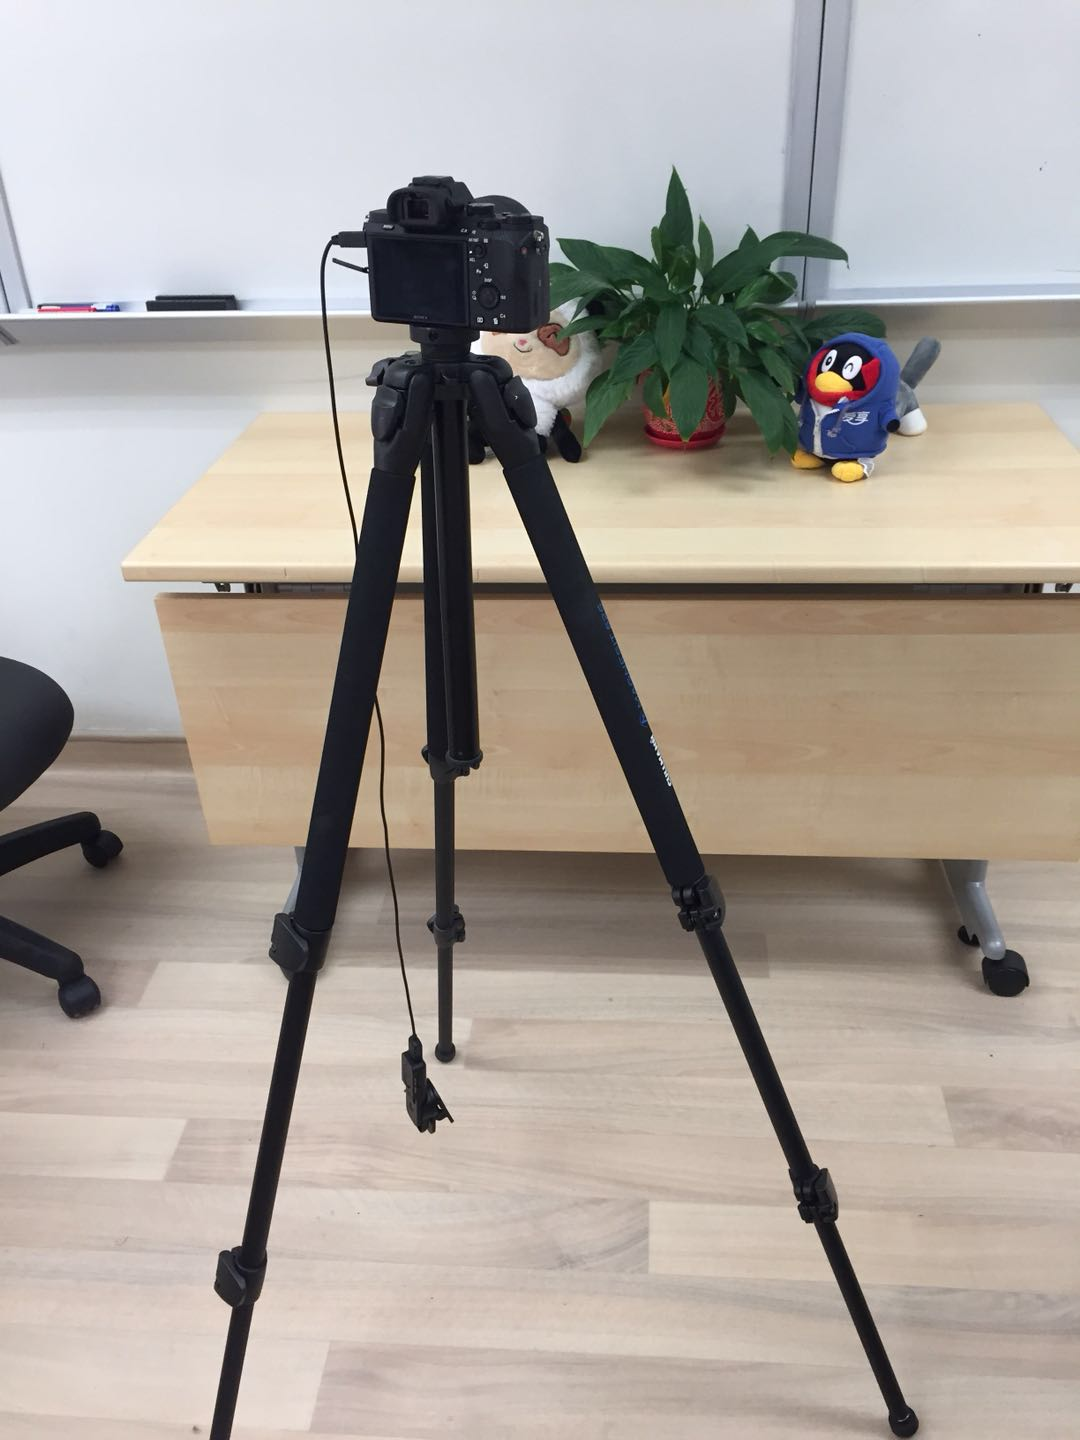
\includegraphics[width=1\textwidth]{images/dataset/scene.jpg}}
\end{minipage}
\begin{minipage}[t]{0.4\textwidth}
\centering
\raisebox{-0.5cm}{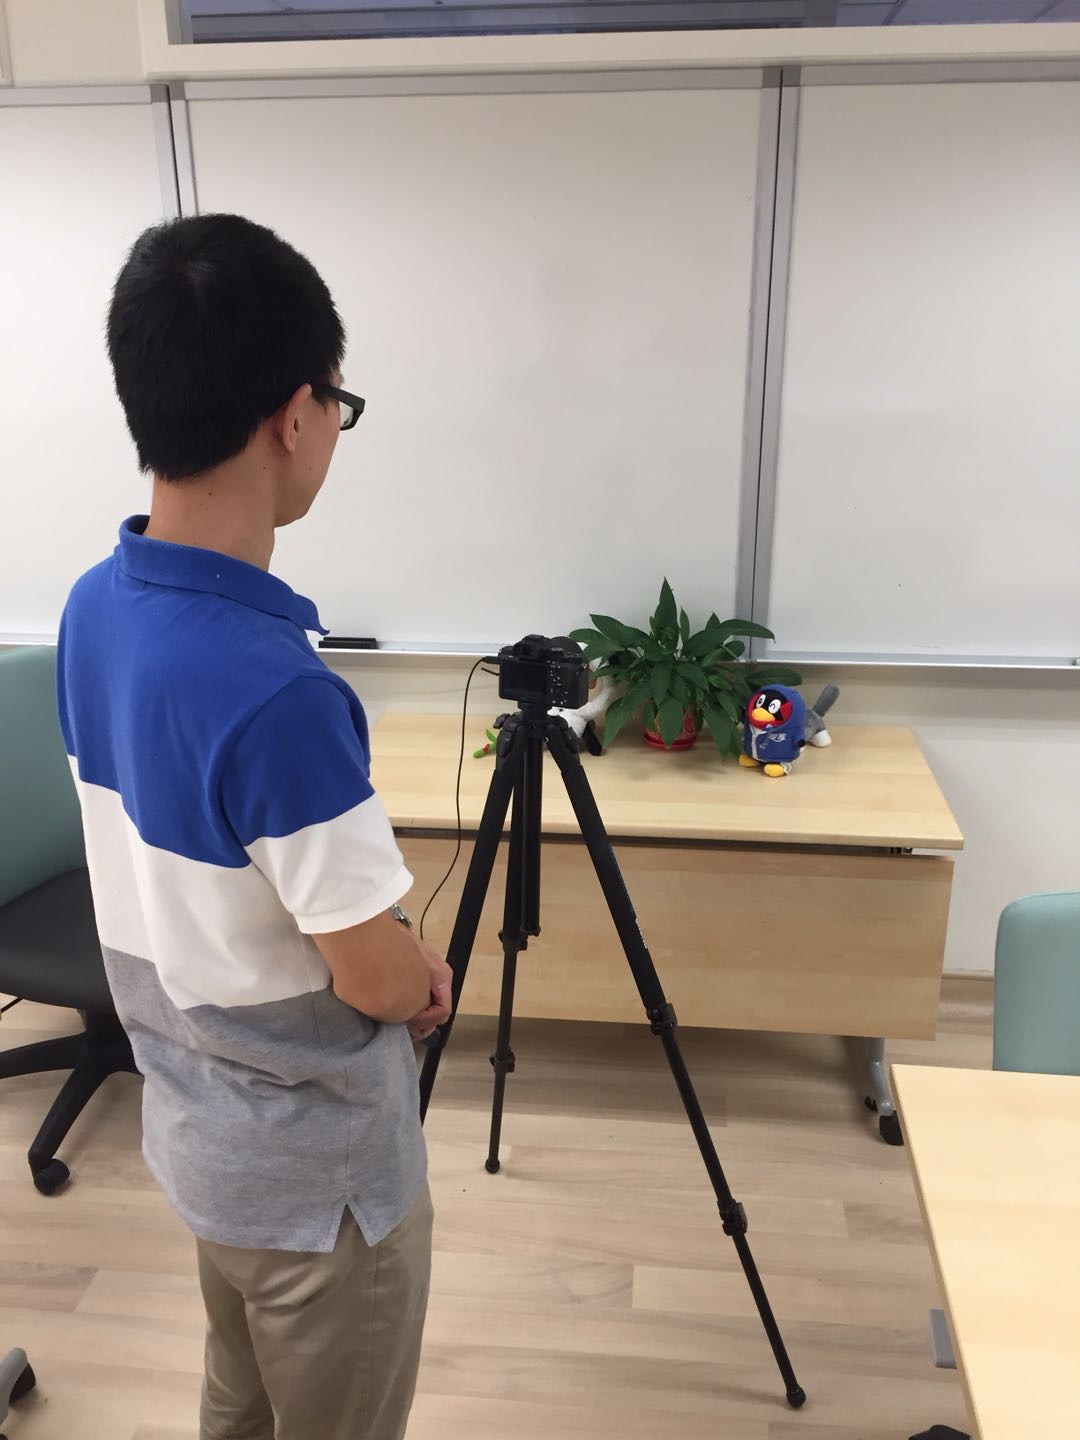
\includegraphics[width=1\textwidth]{images/dataset/scenewithperson.jpg}}
\end{minipage}
}\vspace{-3mm}
    \caption{The static scene is captured with cameras fixed by tripod. The capture is automatically done with shutter release.}
    \label{fig6-2}
\end{figure}

\textbf{More Camera Brands}: In our dataset, we use 5 different cameras of three camera brands, including Canon (Mark 5D, 80D, 600D), Nikon (D800), and Sony (A7 II), to capture real-world noisy images. According to a recent survey \cite{commoncamera}, the three camera brands occupy 48 of 50 most commonly used camera-lens combinations. Hence, our dataset is more comprehensive than the previous datasets in camera brands.

% The other two brands are from the camera brands of Fujifilm and Olympus.

\textbf{More Camera Settings}: In our new dataset, for each camera images are captured with 6 different ISOs, e.g., 800, 1,600, 3,200, 6,400, 12,800, and 25,600. For each ISO value, we carefully adjust the shutter speed and aperture, and choose the most suitable camera setting. With the increase of ISO, the noise levels in the images will also increase. For example, to make the images captured with ISO=25,600 more natural, we set the shutter speed to 1/320 second and aperture to F10.0. Hence, our dataset is more comprehensive at the noise levels than the previous datasets.

\textbf{More Captured Scenes}: We capture the images with indoor normal lighting condition, dark lighting condition, and outdoor normal lighting condition. The scenes we captured are also versaltile (including the buildings, classrooms, caffe rooms, and outdoor scenes). The objects in the scenes include books, pens, bottles, boxes, joys, etc. In summary, we capture totoally 40 different scenes by using 5 different cameras in several different camera settings, including 12 scenes by Canon 5D Mark II, 5 scenes by Canon 80D, 3 scens by Canon 600D, 13 scenes by Nikon D800, 7 scenes by Sony A7 II. Since the images are of large size ($3000\times3000$), we crop some regions from these images and obtain 100 regions of size $512\times512$.

\textbf{Removing Outlier Images}: The outlier images are those images which have misalignment and different illuminance from the base image (we usually choose the first image of the 500 shots as the base image). In the dataset of \cite{crosschannel2016}, the authors did not consider to remove the images with misalignment and different illuminances. In the DND dataset \cite{dnd2017}, the authors considered to correct the misalignment of each image. However, this operation largely depends on the misalignment detection method and the correction method, which may make the corrected images less natural. Besides, the DND dataset \cite{dnd2017} takes the image captured with low ISO as ``ground truth'', and linearly transfer the noisy image captured with high ISO to the scale of the ``ground truth'' image. This step, in our opinion, is problematic since the image pixels are not linearly dependent on the ISO values. In our dataset, we browse the captured images and remove the outlier images with clear misalignment and illuminances. For each scene, three PhD students are employed to do this operation successively, and the remaining images will be used to compute the ``ground truth'' image.
 
\textbf{Generating ``Ground Truth'' Image}: The ``ground truth'' images of the RENOIR dataset \cite{RENOIR2014} are generated when the camera is set with ISO=100, while the other settings are the same as those for the noisy images. The ``ground truth'' images of the dataset \cite{crosschannel2016} are generated by averaging the static images captured on the same scene under the same camera settings. The ``ground truth'' images of the DND dataset \cite{dnd2017} is generated mainly by using low ISO values (e.g., ISO=100), and other post-processing steps include linear intensity changes, spatial misalignment, and low-frequency residual correciton, etc. In our dataset, we employ the method of \cite{crosschannel2016} due to its simplisity. We capture images the same of static scenes for many ($500\sim1000$) times and average the captured images to get the clean ``ground truth'' image. 

We first remove the images with misalignment by careful subjective evaluation. The images with several pixels displacement will be deleted. After this stage, we will then remove the images with inconsistant illuminance. The illuminance is affected by two factors. One is that the captured scenes are influenced by the lighting conditions of the environment. The other is that the camera will automatically make up the illuminance when the scene are in a relatively low lighting condition. Since we shot the scene for many times, some shots may have different illumination, though captured under the same lighting condition. To remove the images with outlier illuminance, we first sample 10,000 pixels uniformly (the pixels are on the 100 equidistantly sampled rows and 100 equidistantly sampled columns) from each image, and then compute the mean illuminance of the 10,000 pixels. Each of the captured images will have one value representing its mean illuminances. We sort these values in a descending order. The images with the lowest or highest mean illuminances will be refered as outlier images. We remove these images until the lowest and highest mean illuminances are close enough to the ``center'' of the mean illuminances. Here, ``center'' means the middle of the sorted mean values or mean illuminances. In this way, the images which are much darker or much brighter than the image with the mean illuminance will be removed and the remaining images are very close to each other. The remaining images will be averaged to obtain the mean image, which will be used as the ``ground truth'' image of each scene.

\subsection{Summary of the Dataset}

In our constructed dataset, we captured images from 40 different scenes with different contents and objects. In Figure \ref{fig6-3}, we show some samples of the real-world noisy images we captured in the dataset. For example, we captured the scenes from different types of classrooms, various types of indoor scenes, and versaitile objects under fixed lighting conditions, etc.

\begin{figure}[t!]
    \centering
\subfigure{
\begin{minipage}[t]{0.4\textwidth}
\centering
\raisebox{-0.5cm}{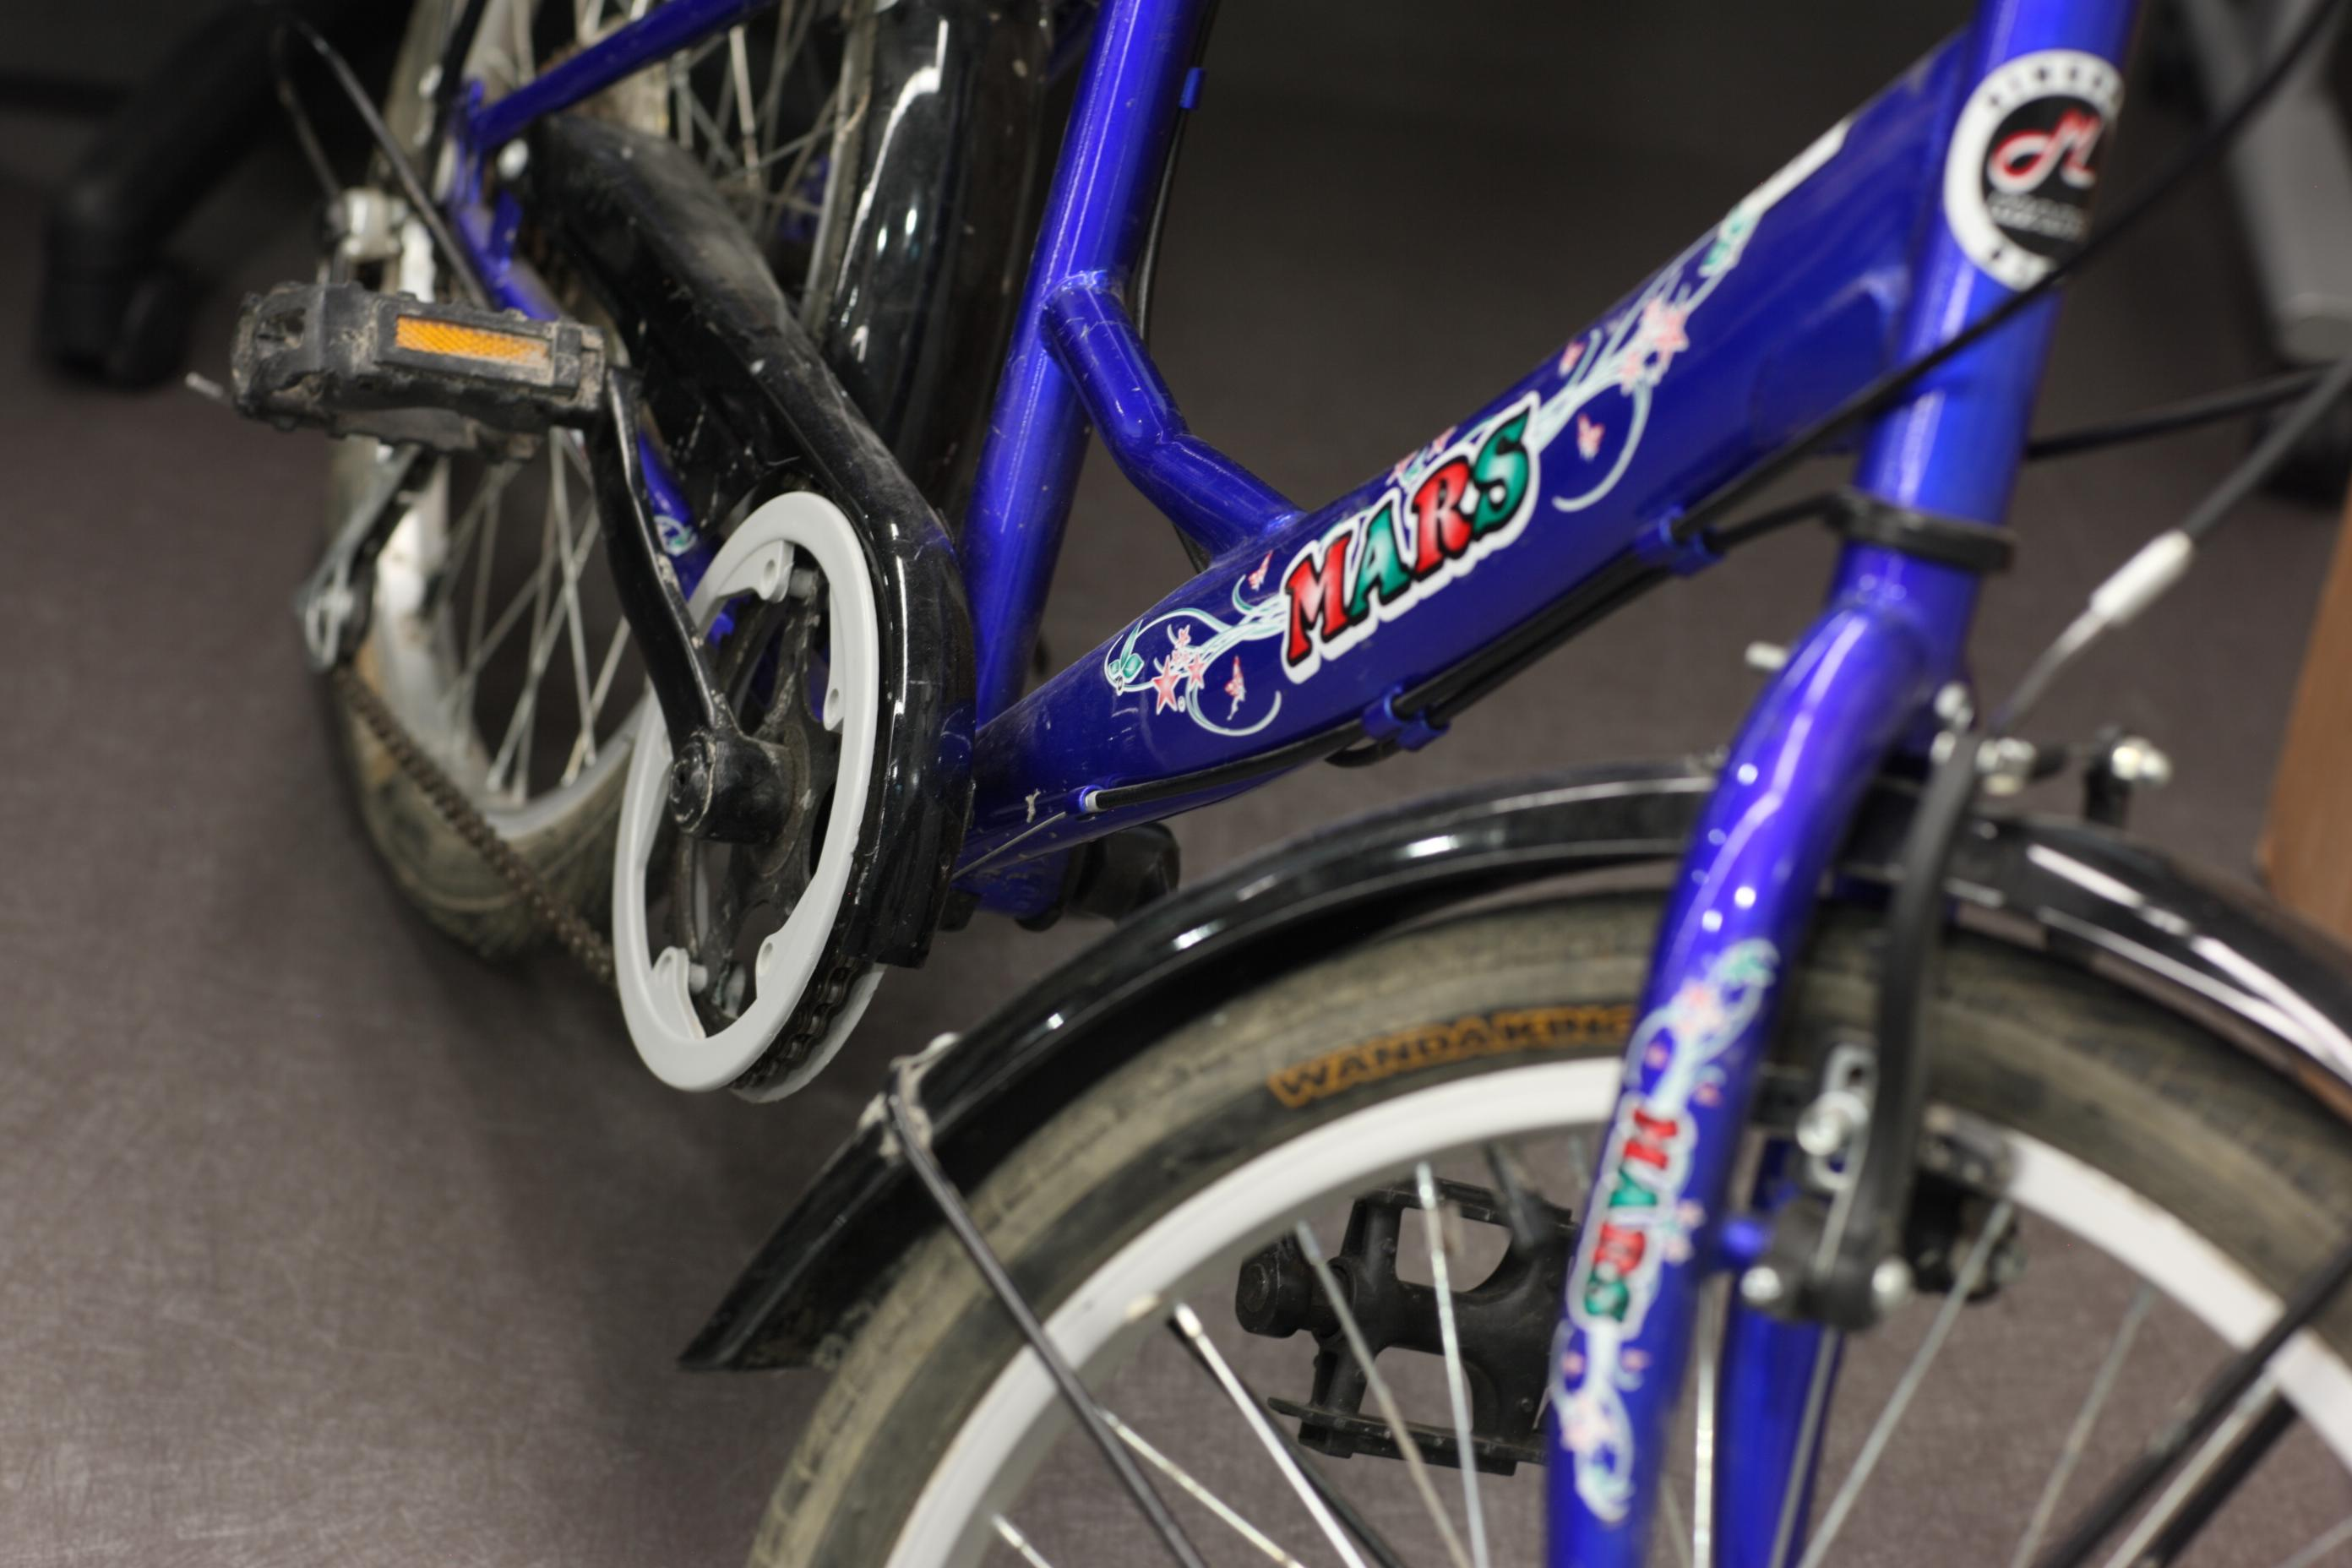
\includegraphics[width=1\textwidth]{images/dataset/Canon5D2_5_160_6400_bicycle_mean.JPG}}
\end{minipage}
\begin{minipage}[t]{0.4\textwidth}
\centering
\raisebox{-0.5cm}{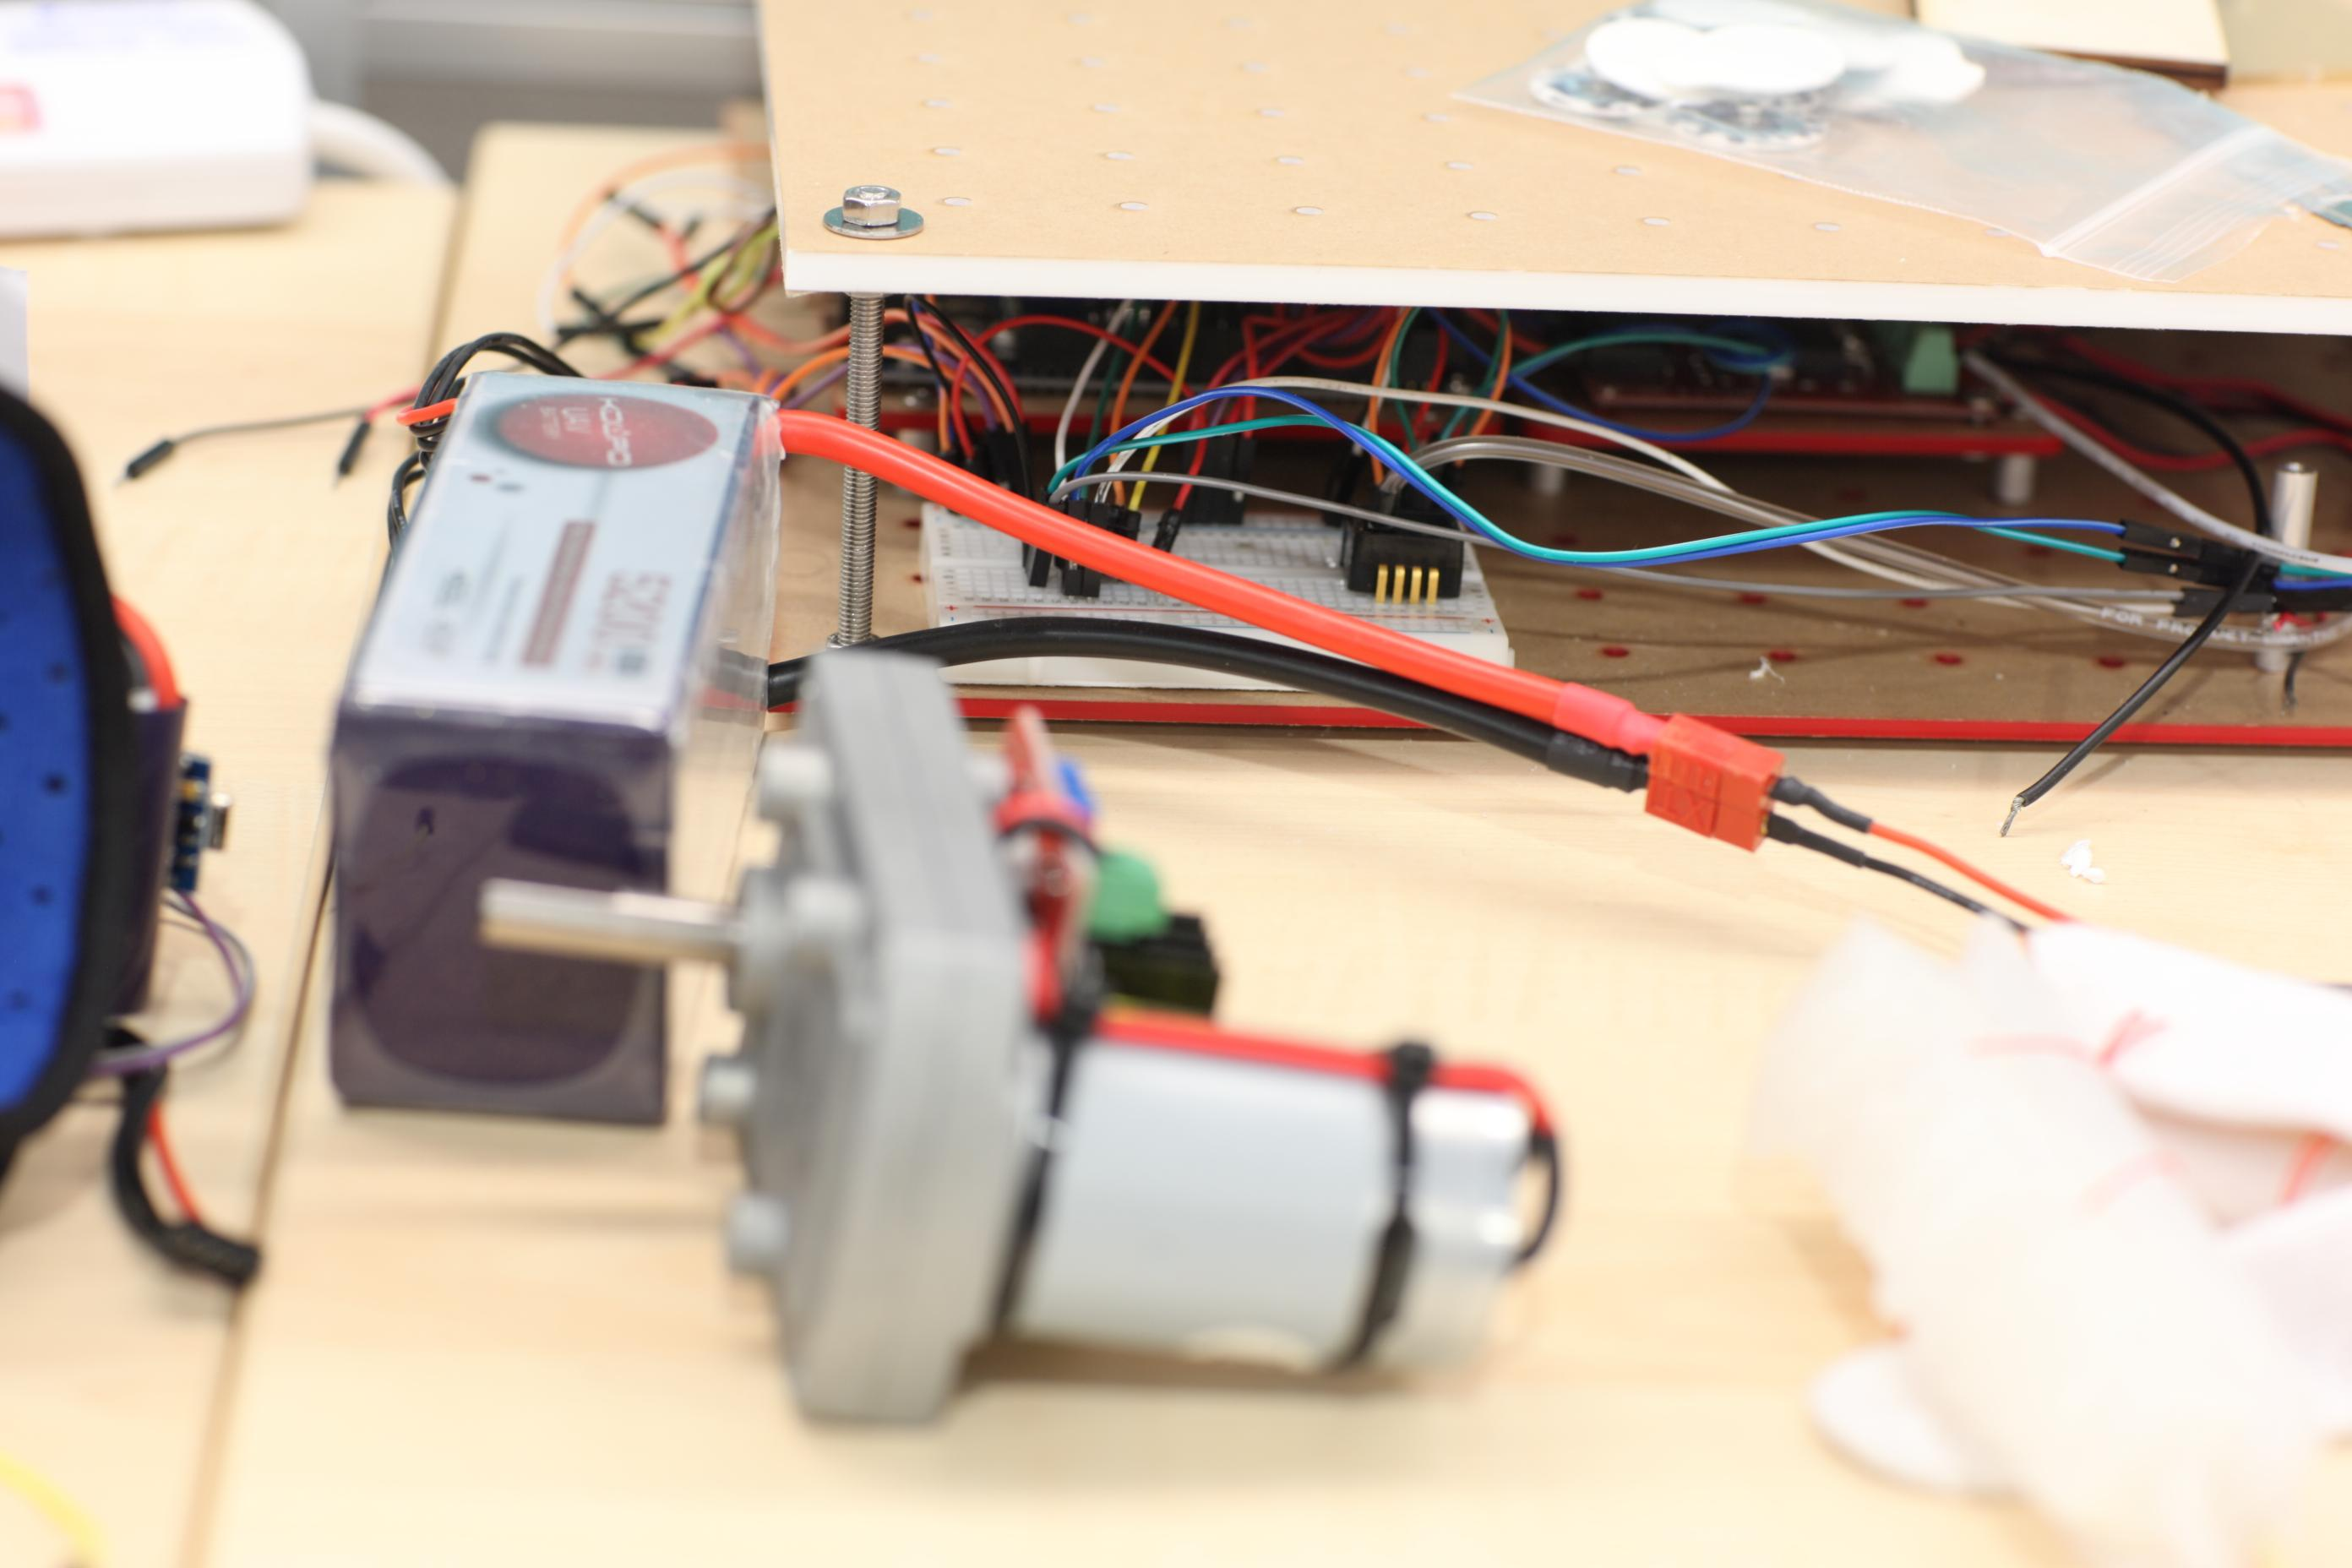
\includegraphics[width=1\textwidth]{images/dataset/Canon5D2_5_160_6400_circuit_mean.JPG}}
\end{minipage}
}\vspace{-3mm}
\subfigure{
\begin{minipage}[t]{0.4\textwidth}
\centering
\raisebox{-0.5cm}{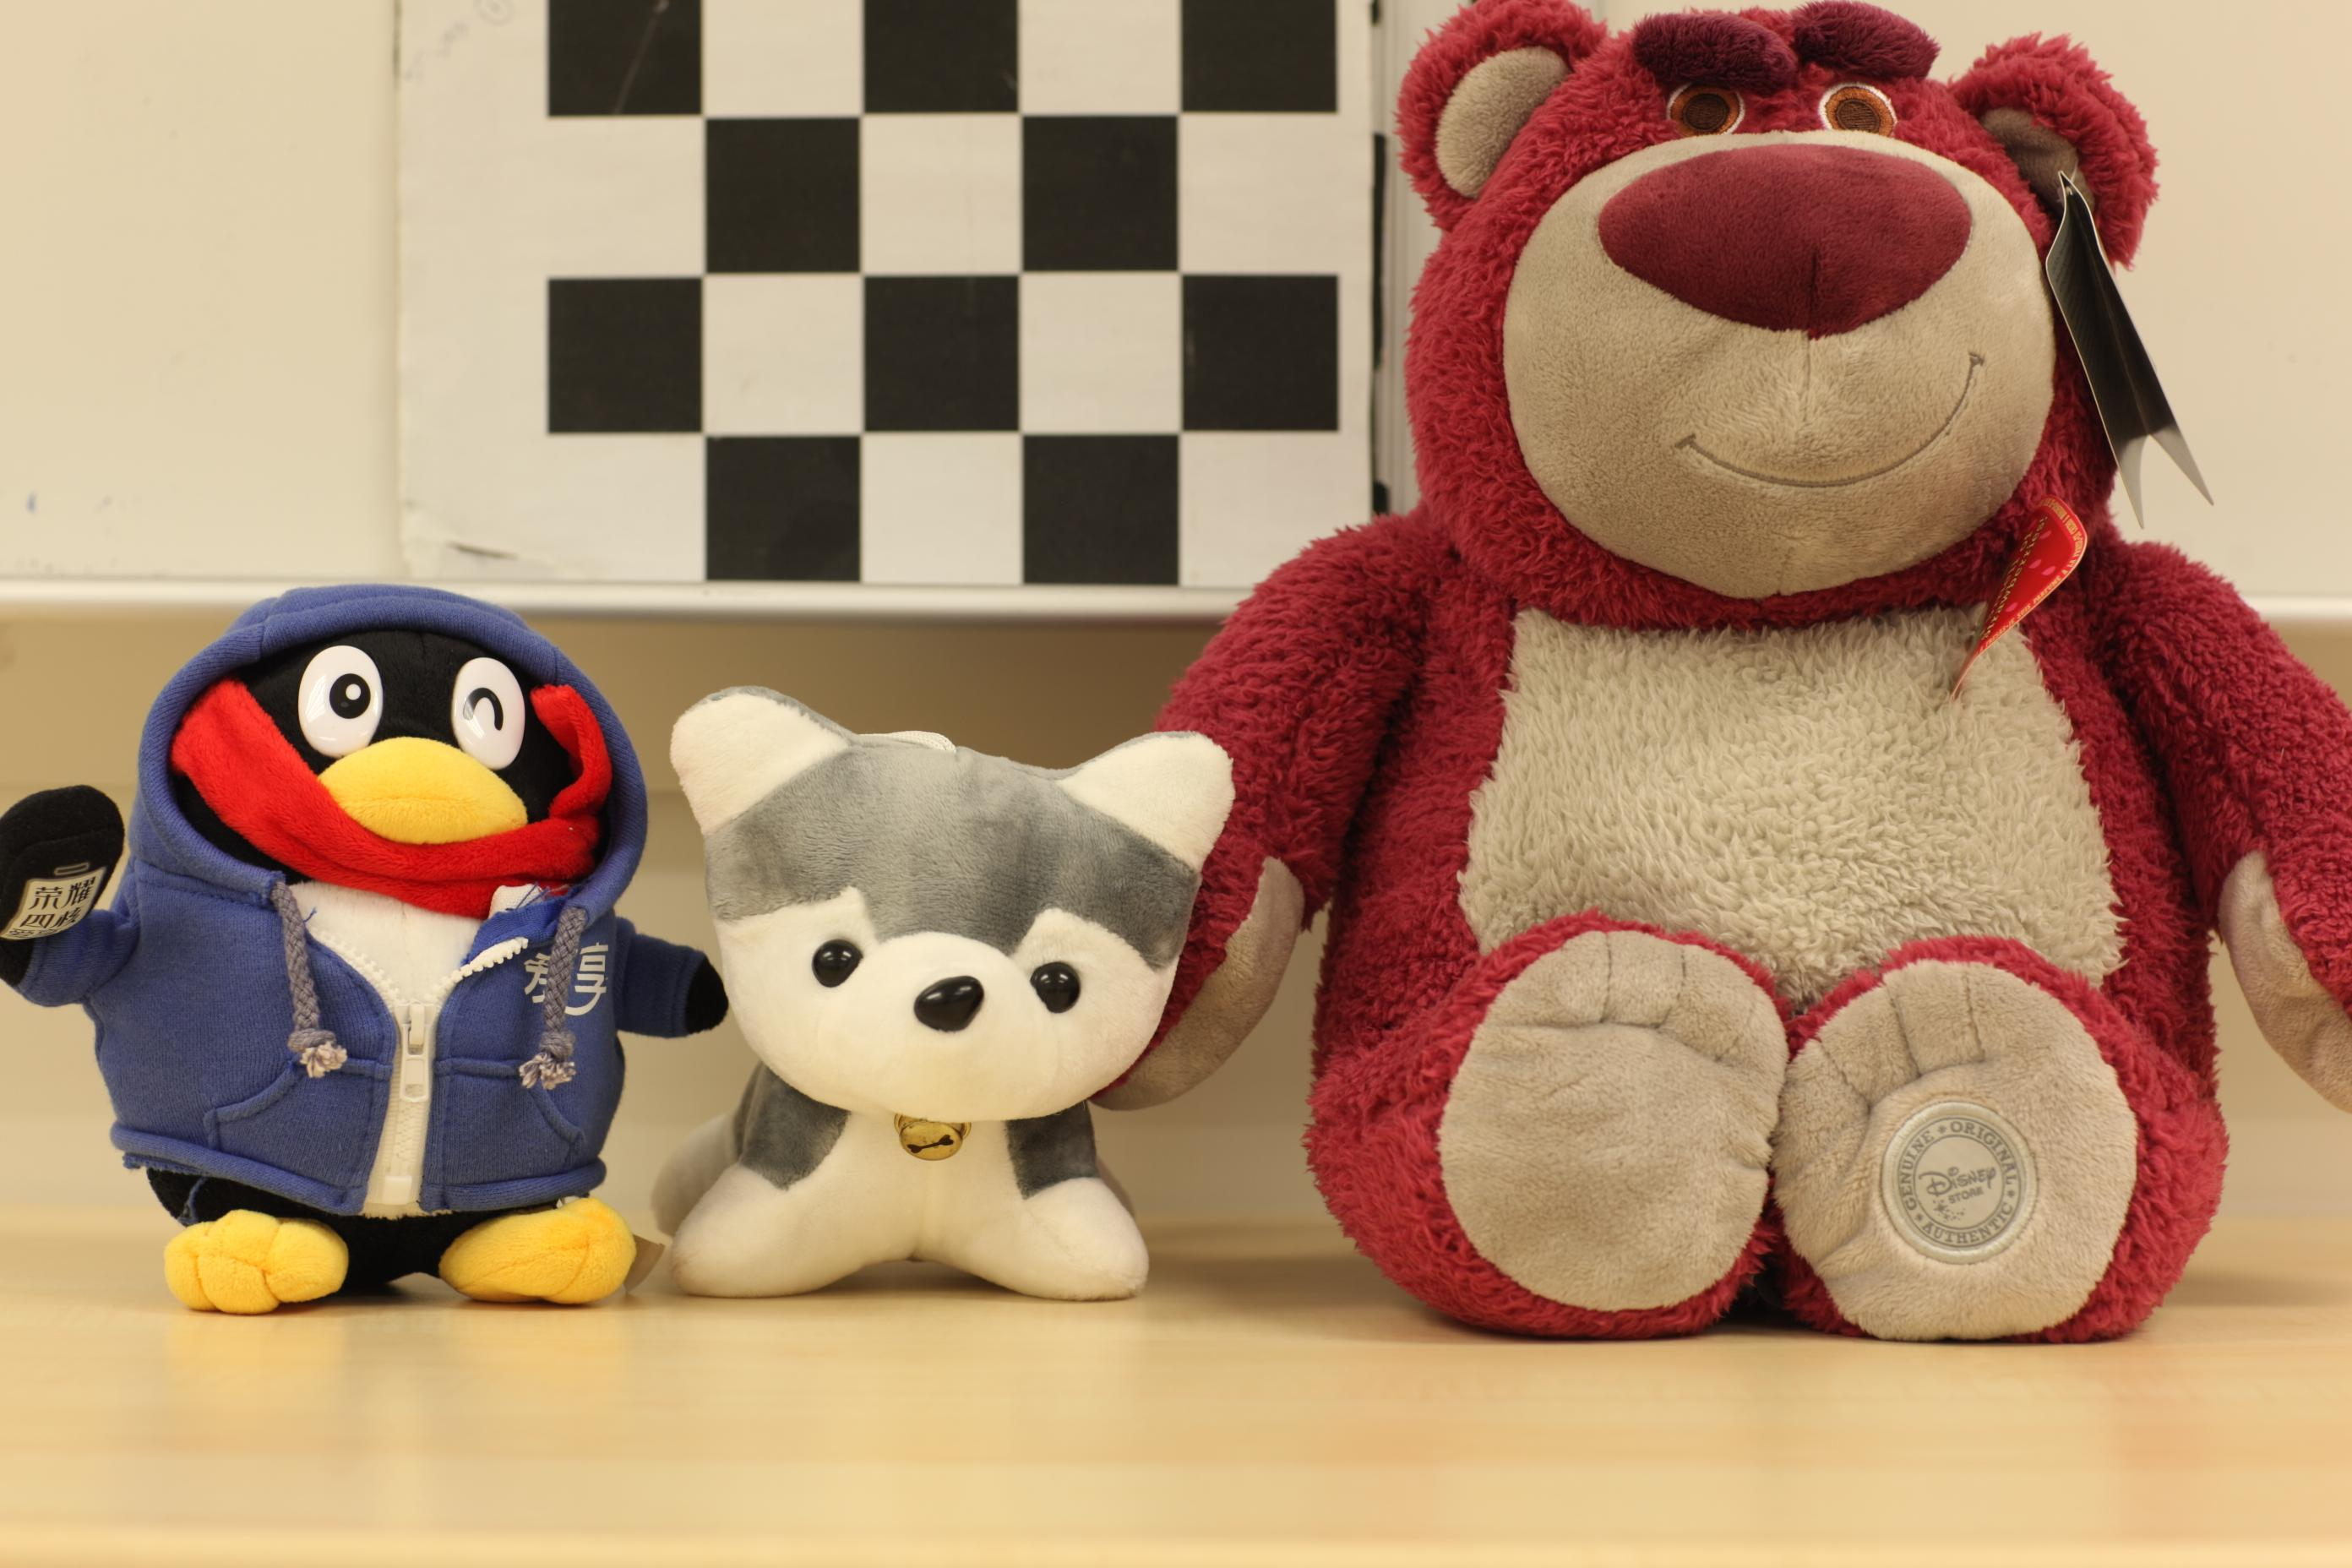
\includegraphics[width=1\textwidth]{images/dataset/Canon5D2_5_200_3200_toy_mean.JPG}}
\end{minipage}
\begin{minipage}[t]{0.4\textwidth}
\centering
\raisebox{-0.5cm}{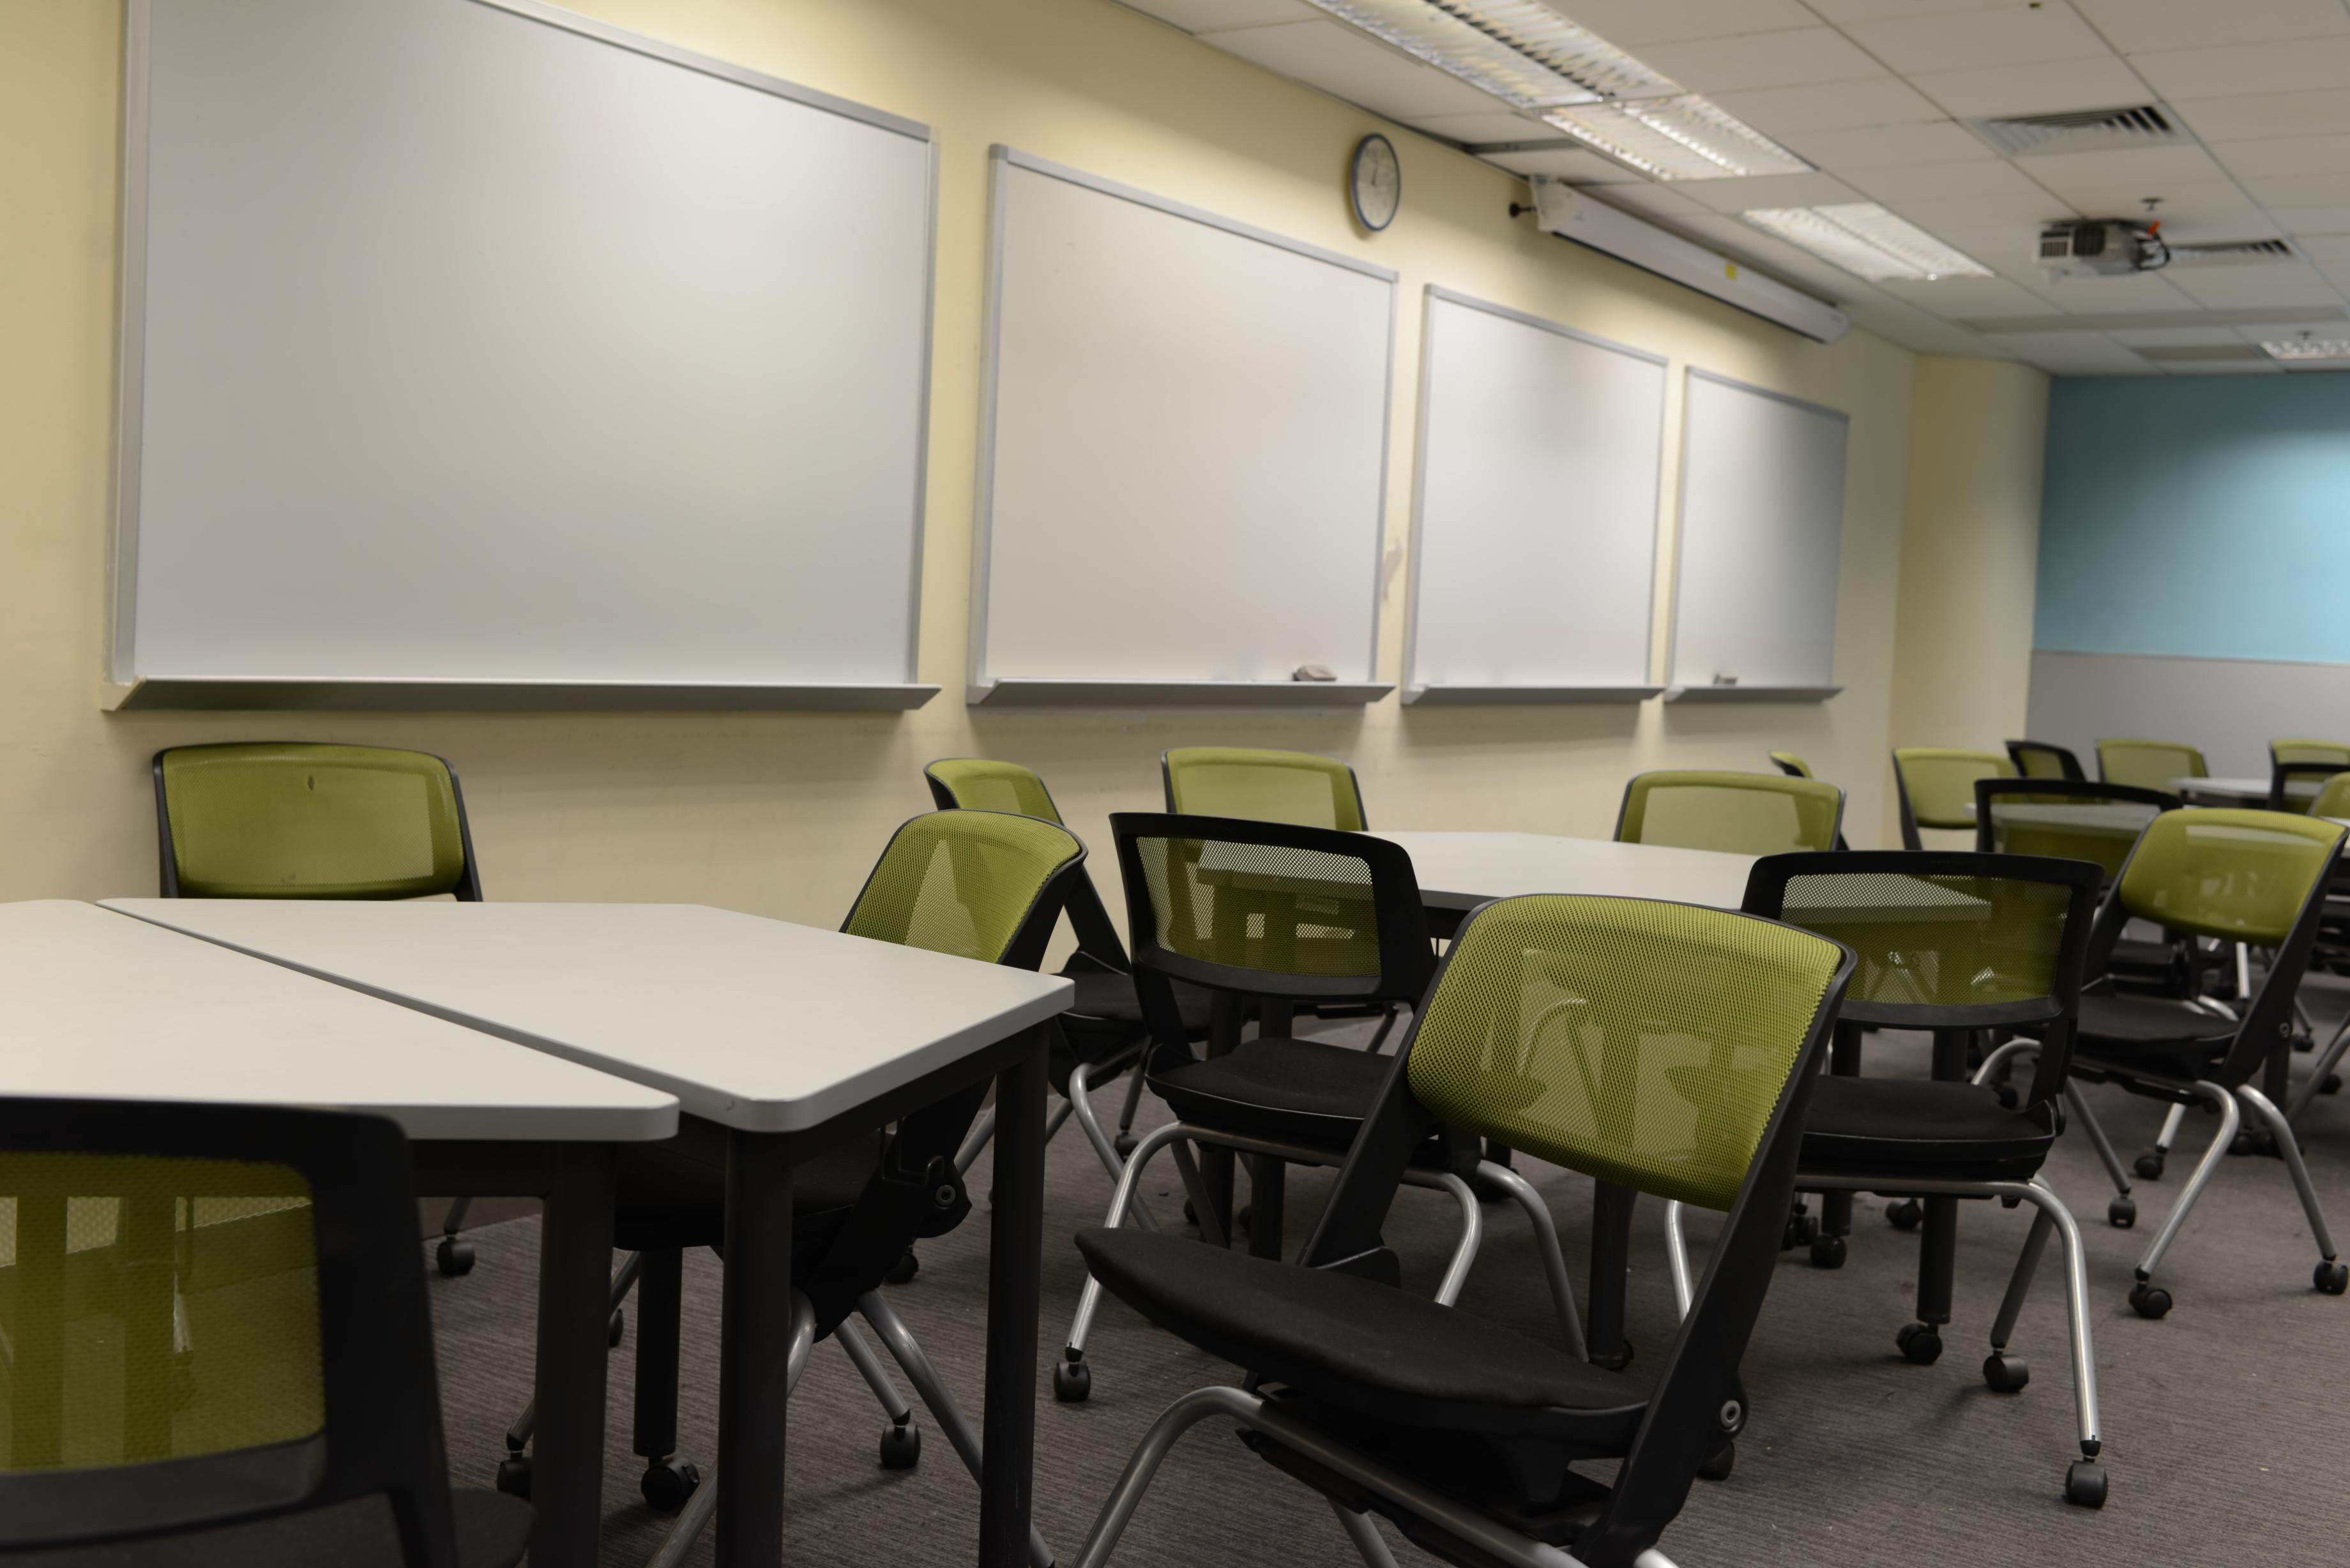
\includegraphics[width=1\textwidth]{images/dataset/NikonD800_4-5_160_1800_classroom_mean.JPG}}
\end{minipage}
}\vspace{-3mm}
\subfigure{
\begin{minipage}[t]{0.4\textwidth}
\centering
\raisebox{-0.5cm}{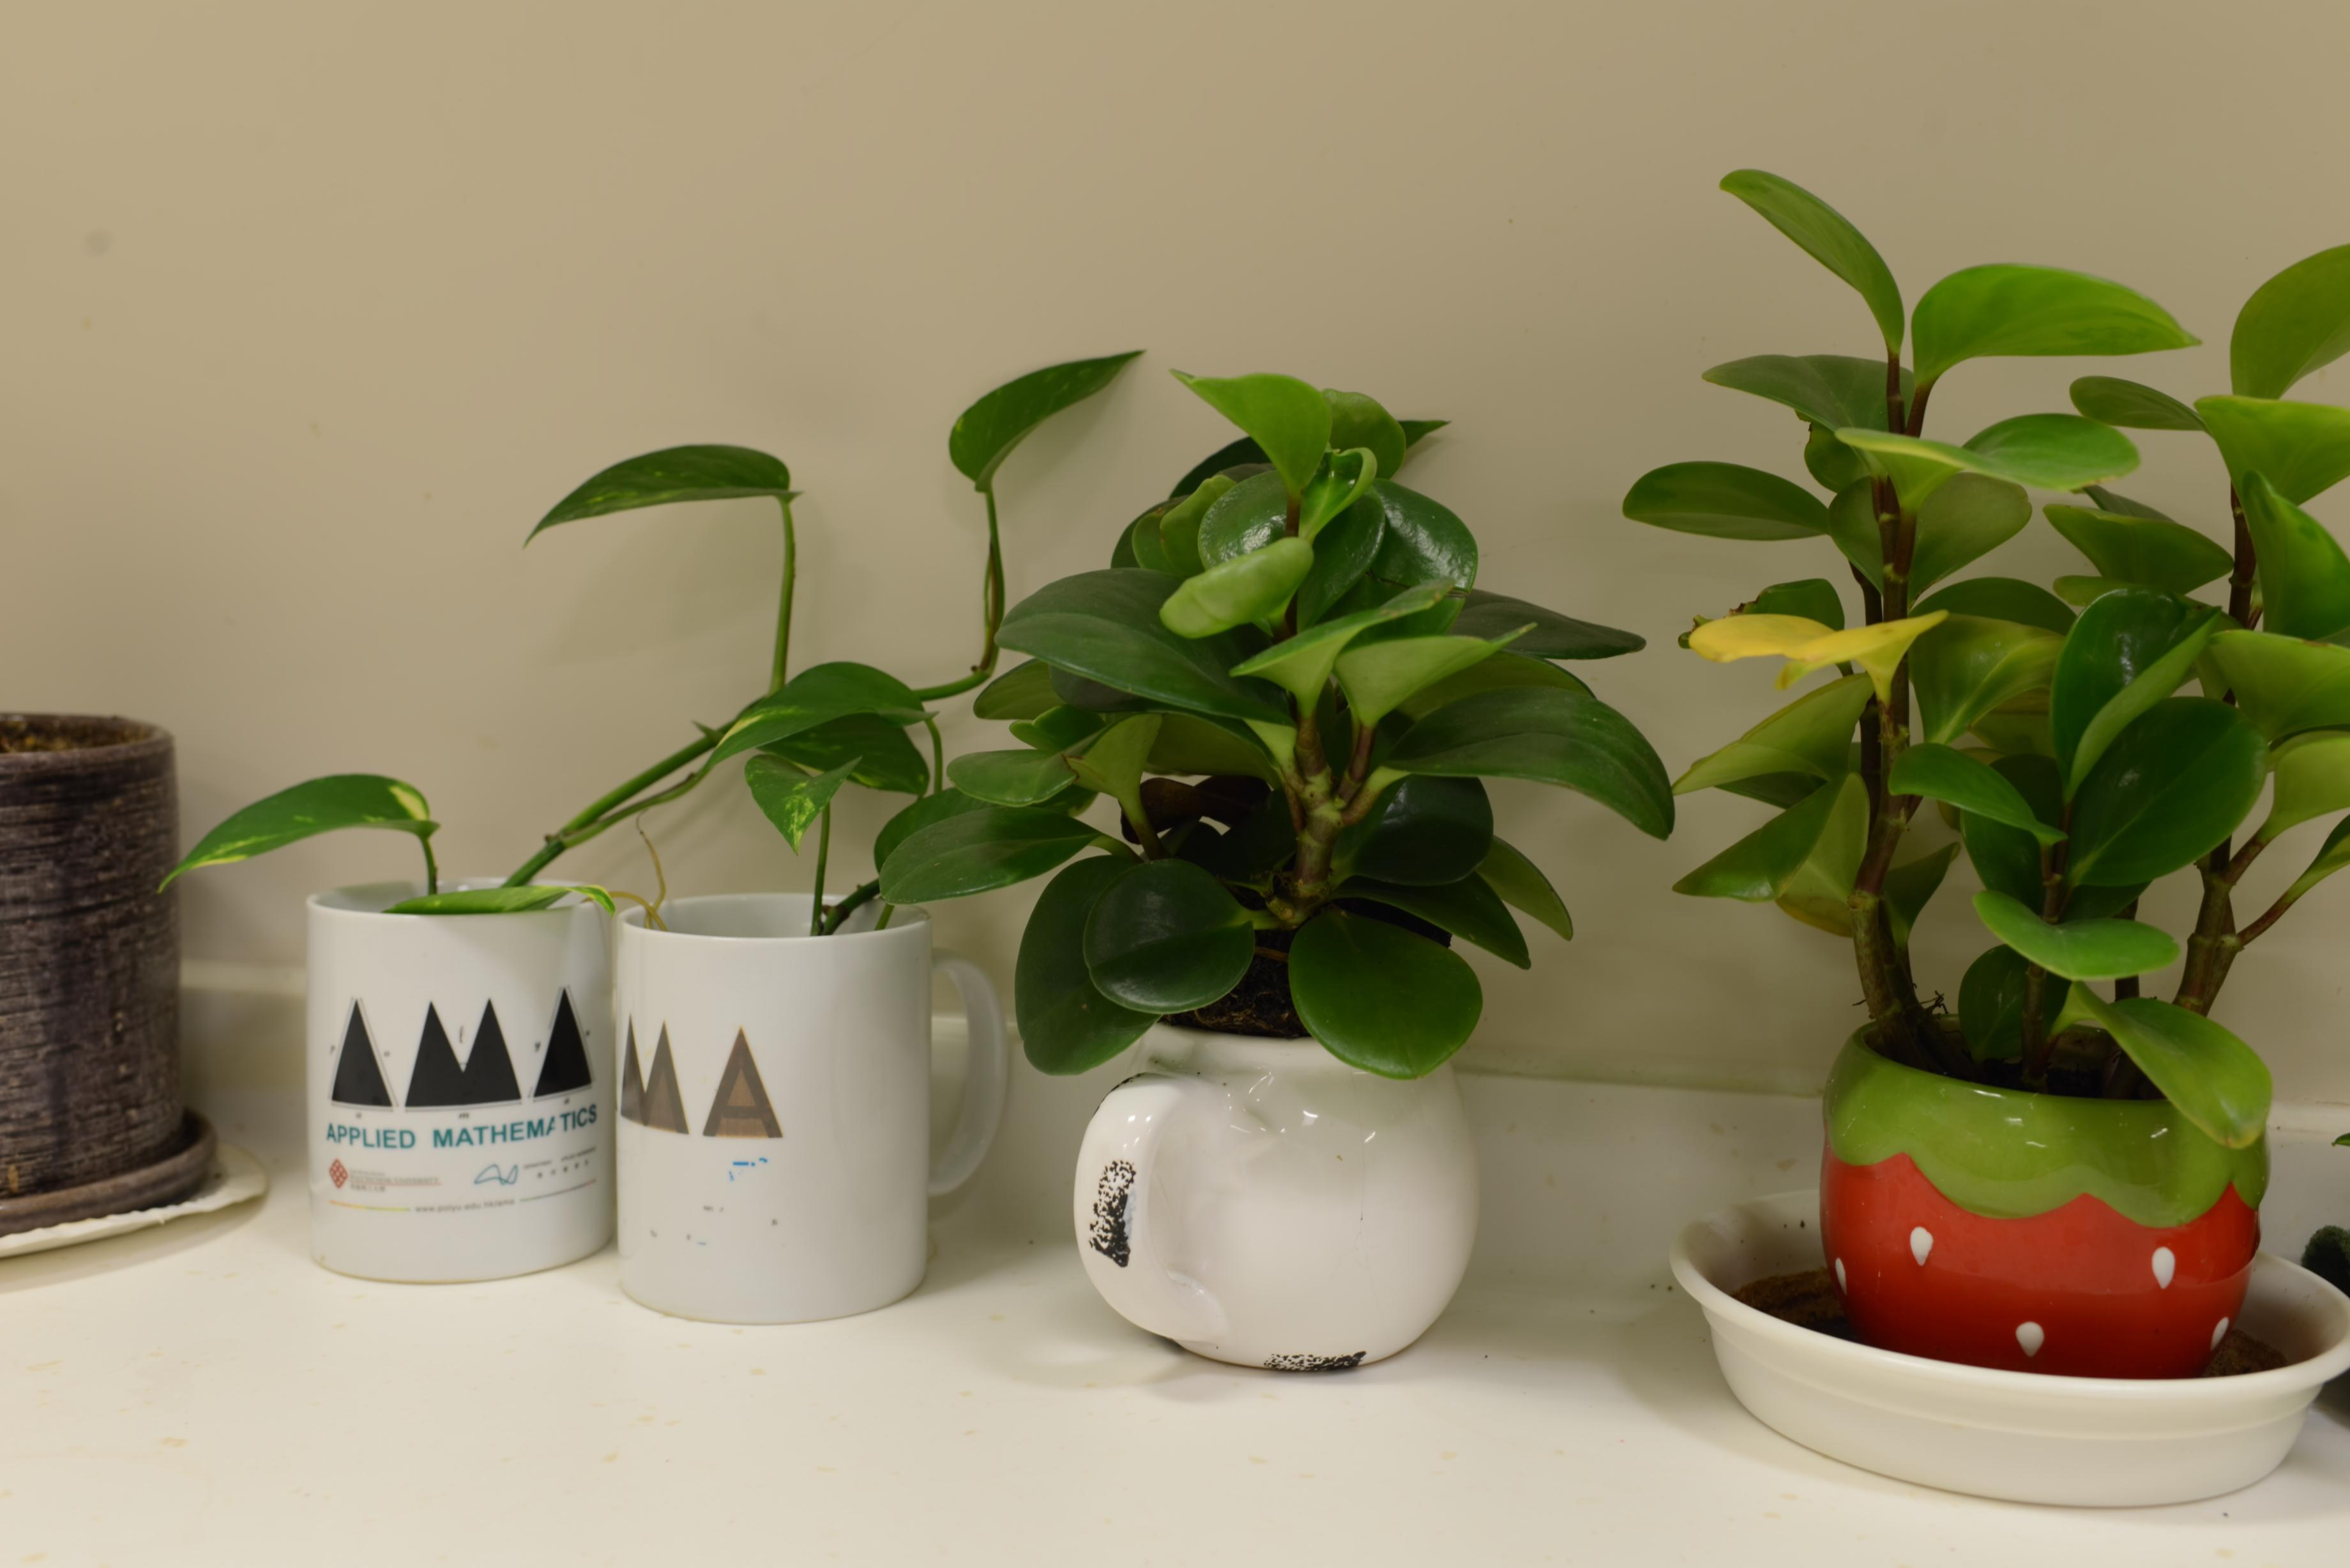
\includegraphics[width=1\textwidth]{images/dataset/NikonD800_6-3_125_5000_plant_mean.JPG}}
\end{minipage}
\begin{minipage}[t]{0.4\textwidth}
\centering
\raisebox{-0.5cm}{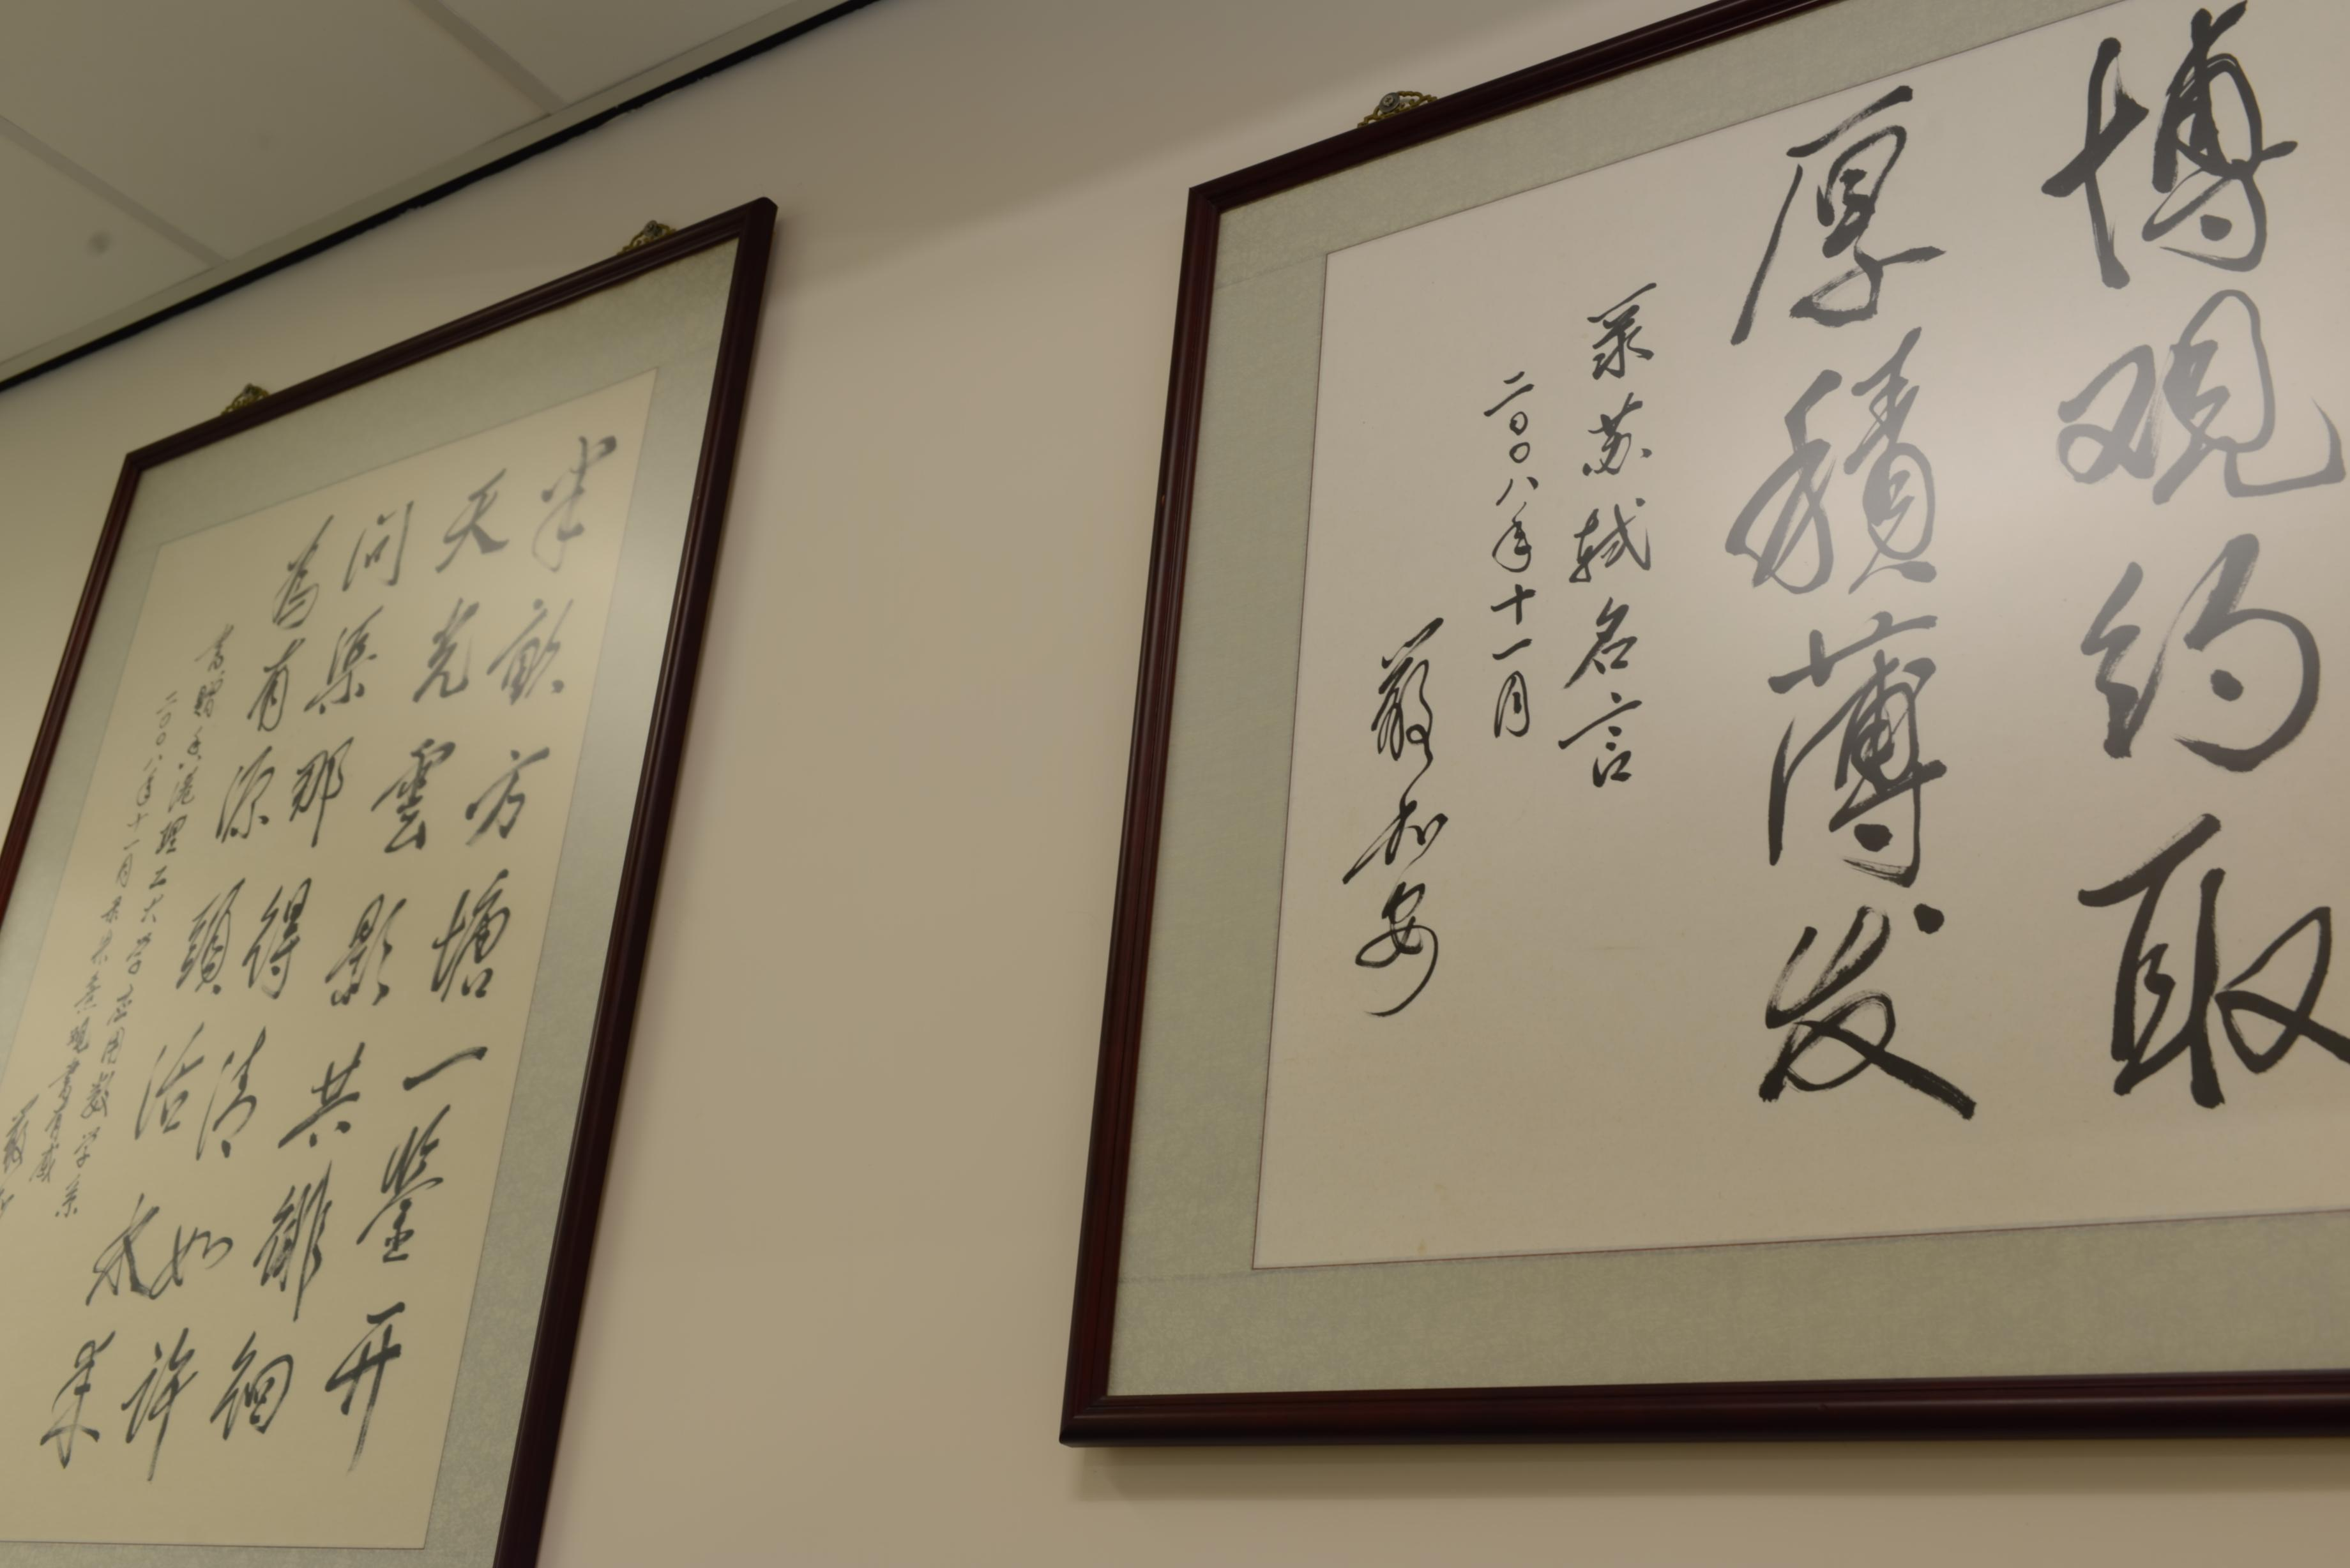
\includegraphics[width=1\textwidth]{images/dataset/NikonD800_8_125_6400_photo_mean.JPG}}
\end{minipage}
}\vspace{-3mm}
\subfigure{
\begin{minipage}[t]{0.4\textwidth}
\centering
\raisebox{-0.5cm}{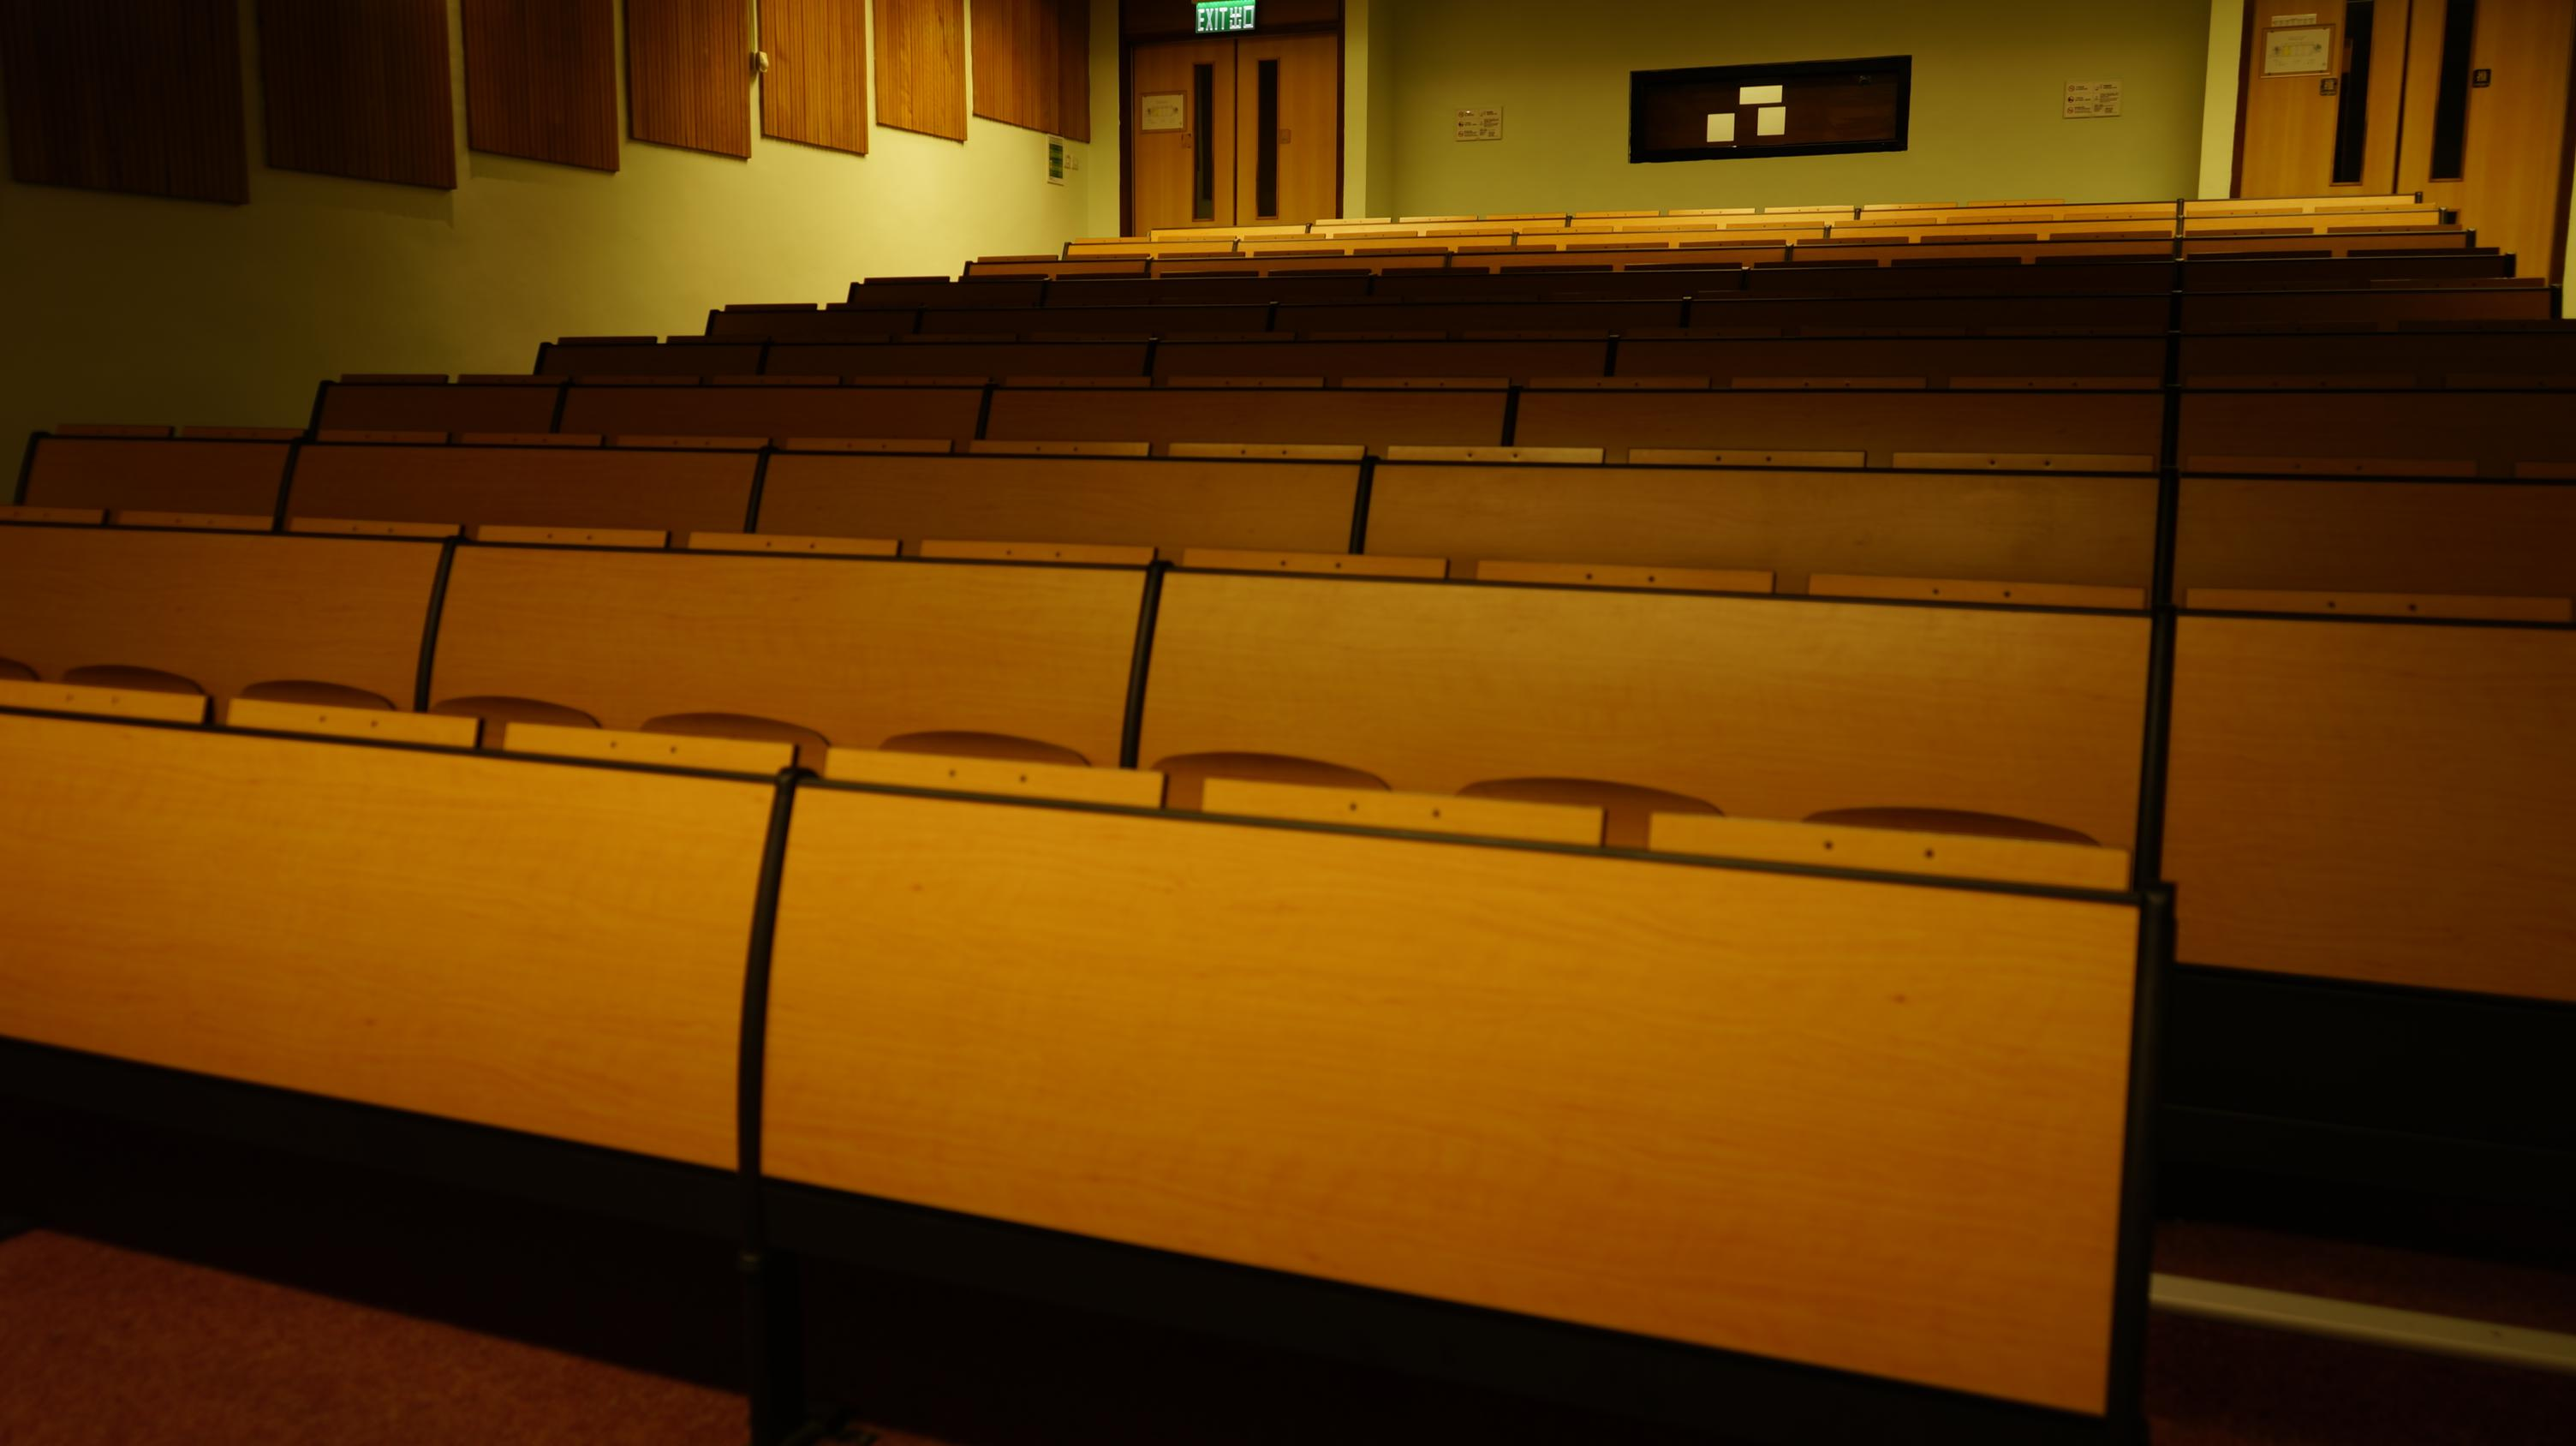
\includegraphics[width=1\textwidth]{images/dataset/Sony_3-5_200_1600_classroom_mean.JPG}}
\end{minipage}
\begin{minipage}[t]{0.4\textwidth}
\centering
\raisebox{-0.5cm}{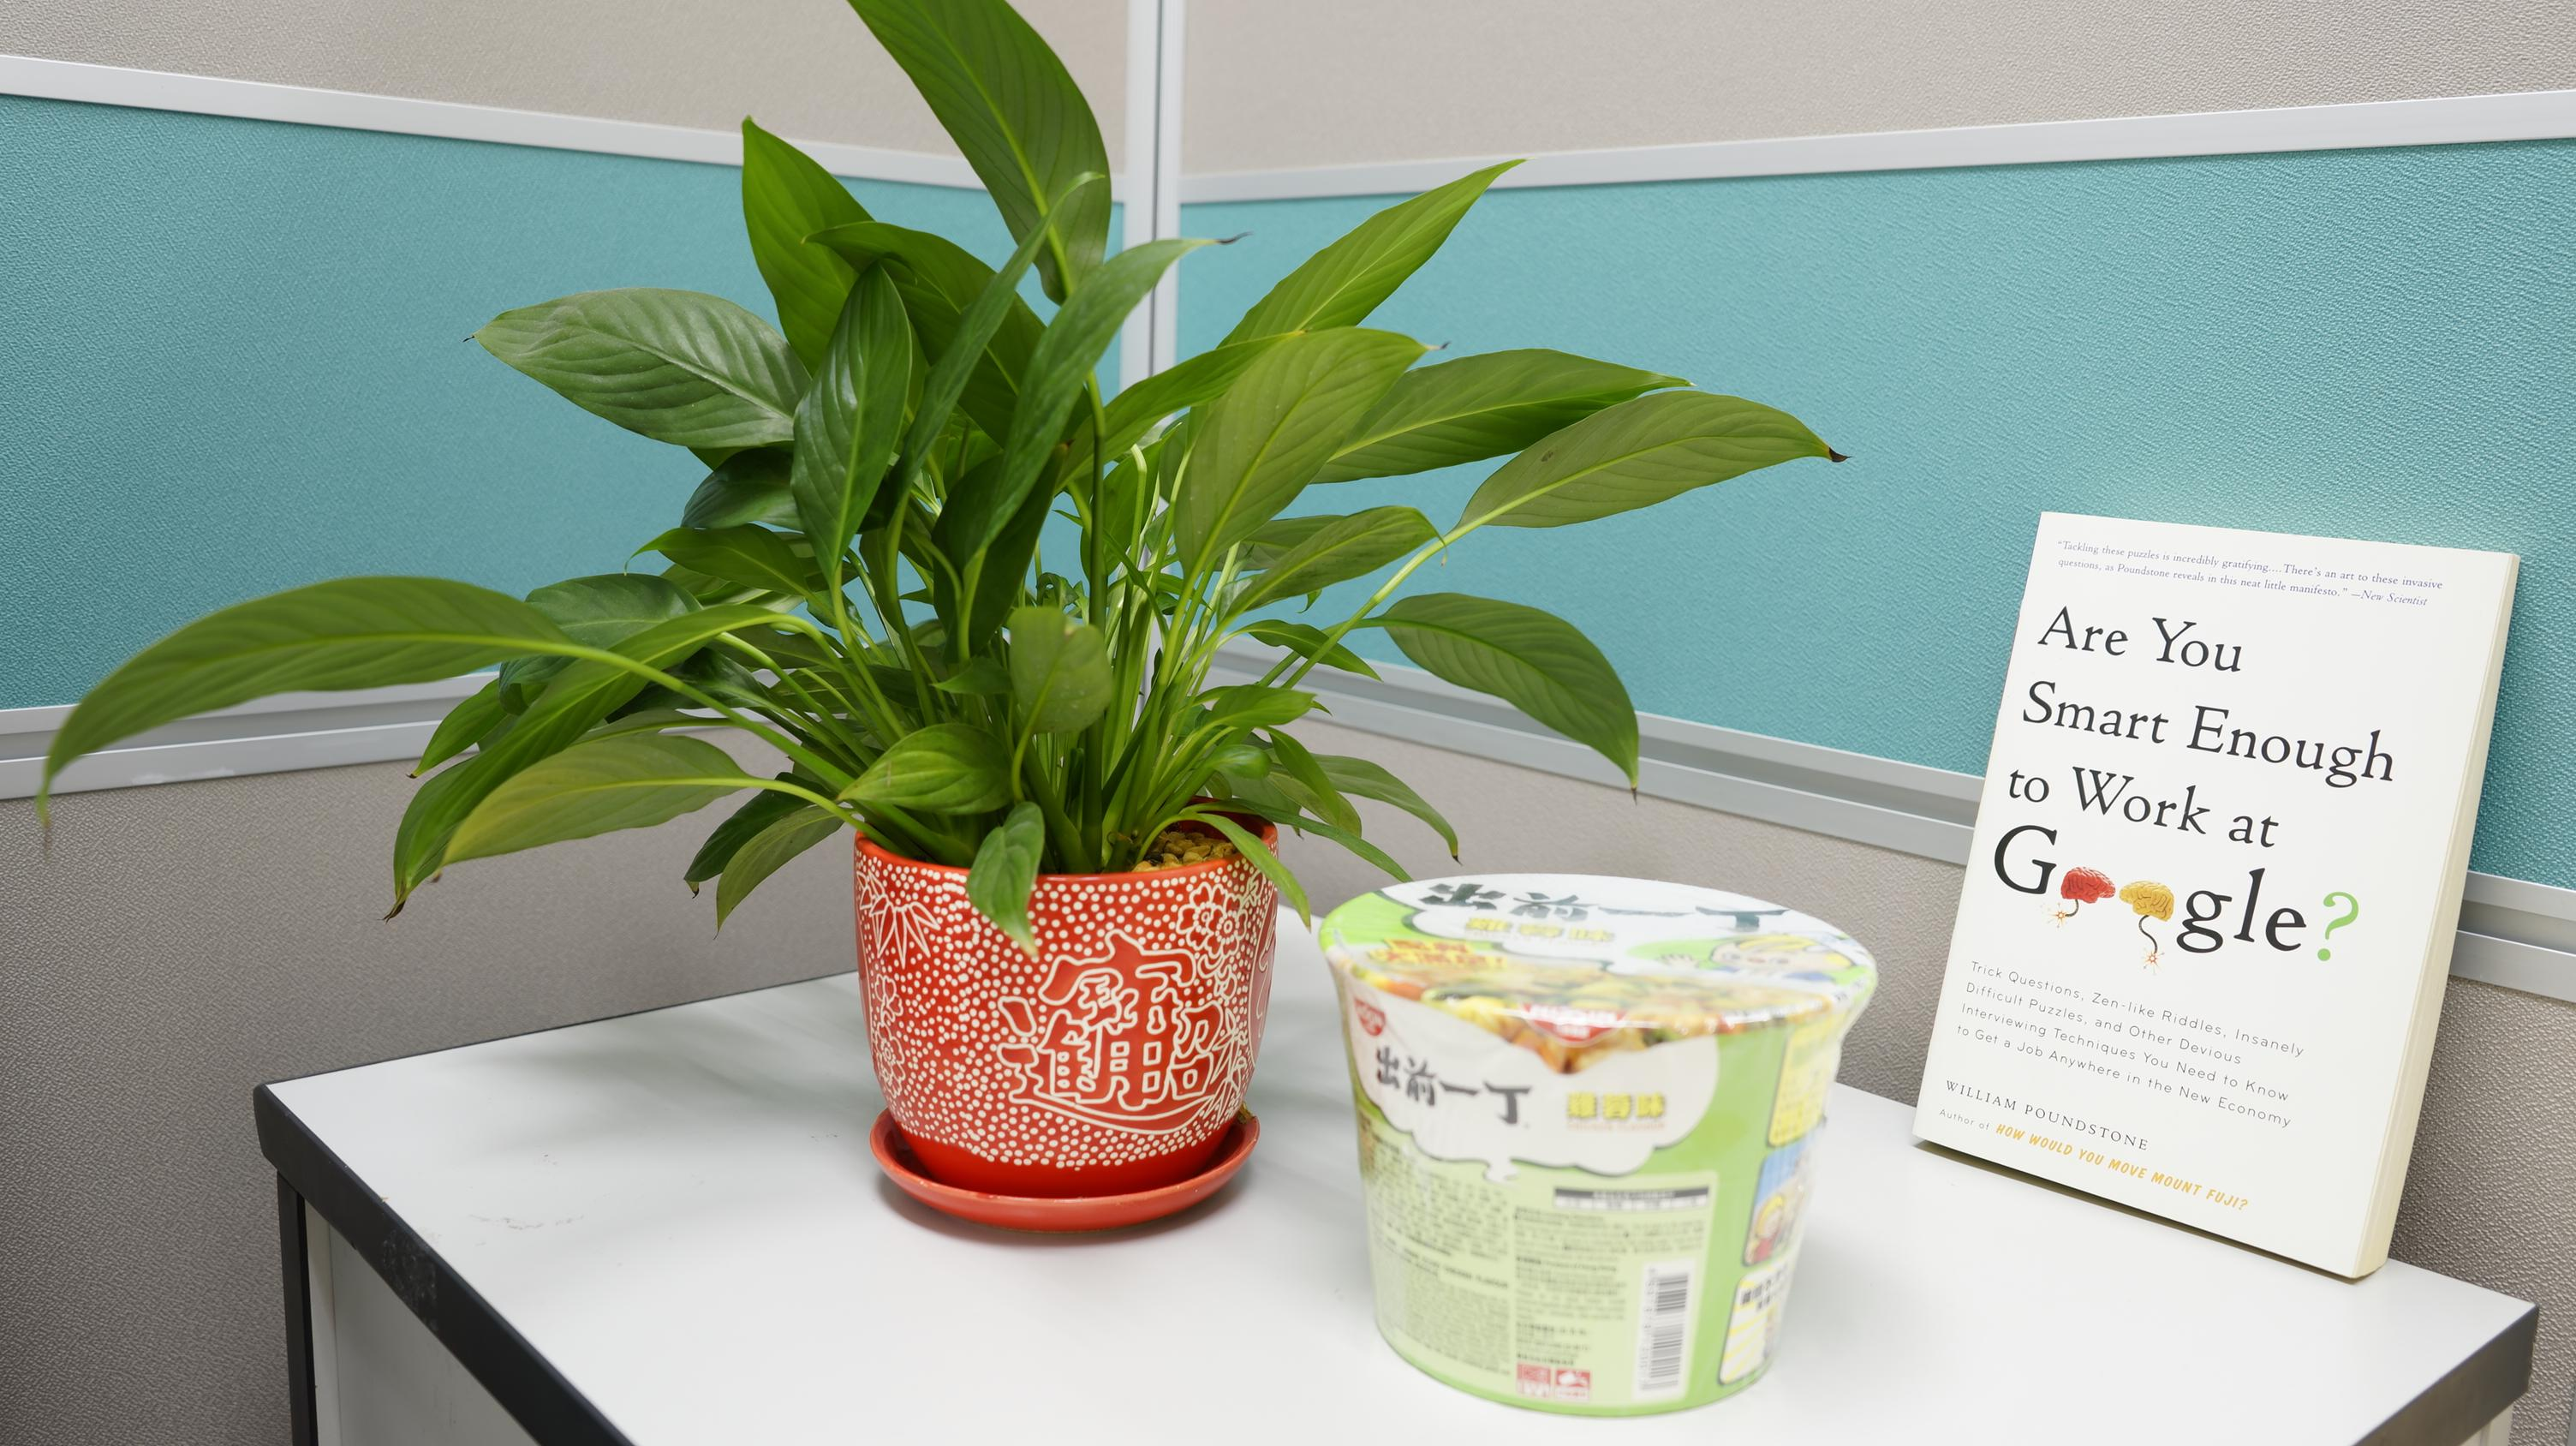
\includegraphics[width=1\textwidth]{images/dataset/Sony_4-5_125_3200_plant_mean.JPG}}
\end{minipage}
}\vspace{-3mm}
\subfigure{
\begin{minipage}[t]{0.4\textwidth}
\centering
\raisebox{-0.5cm}{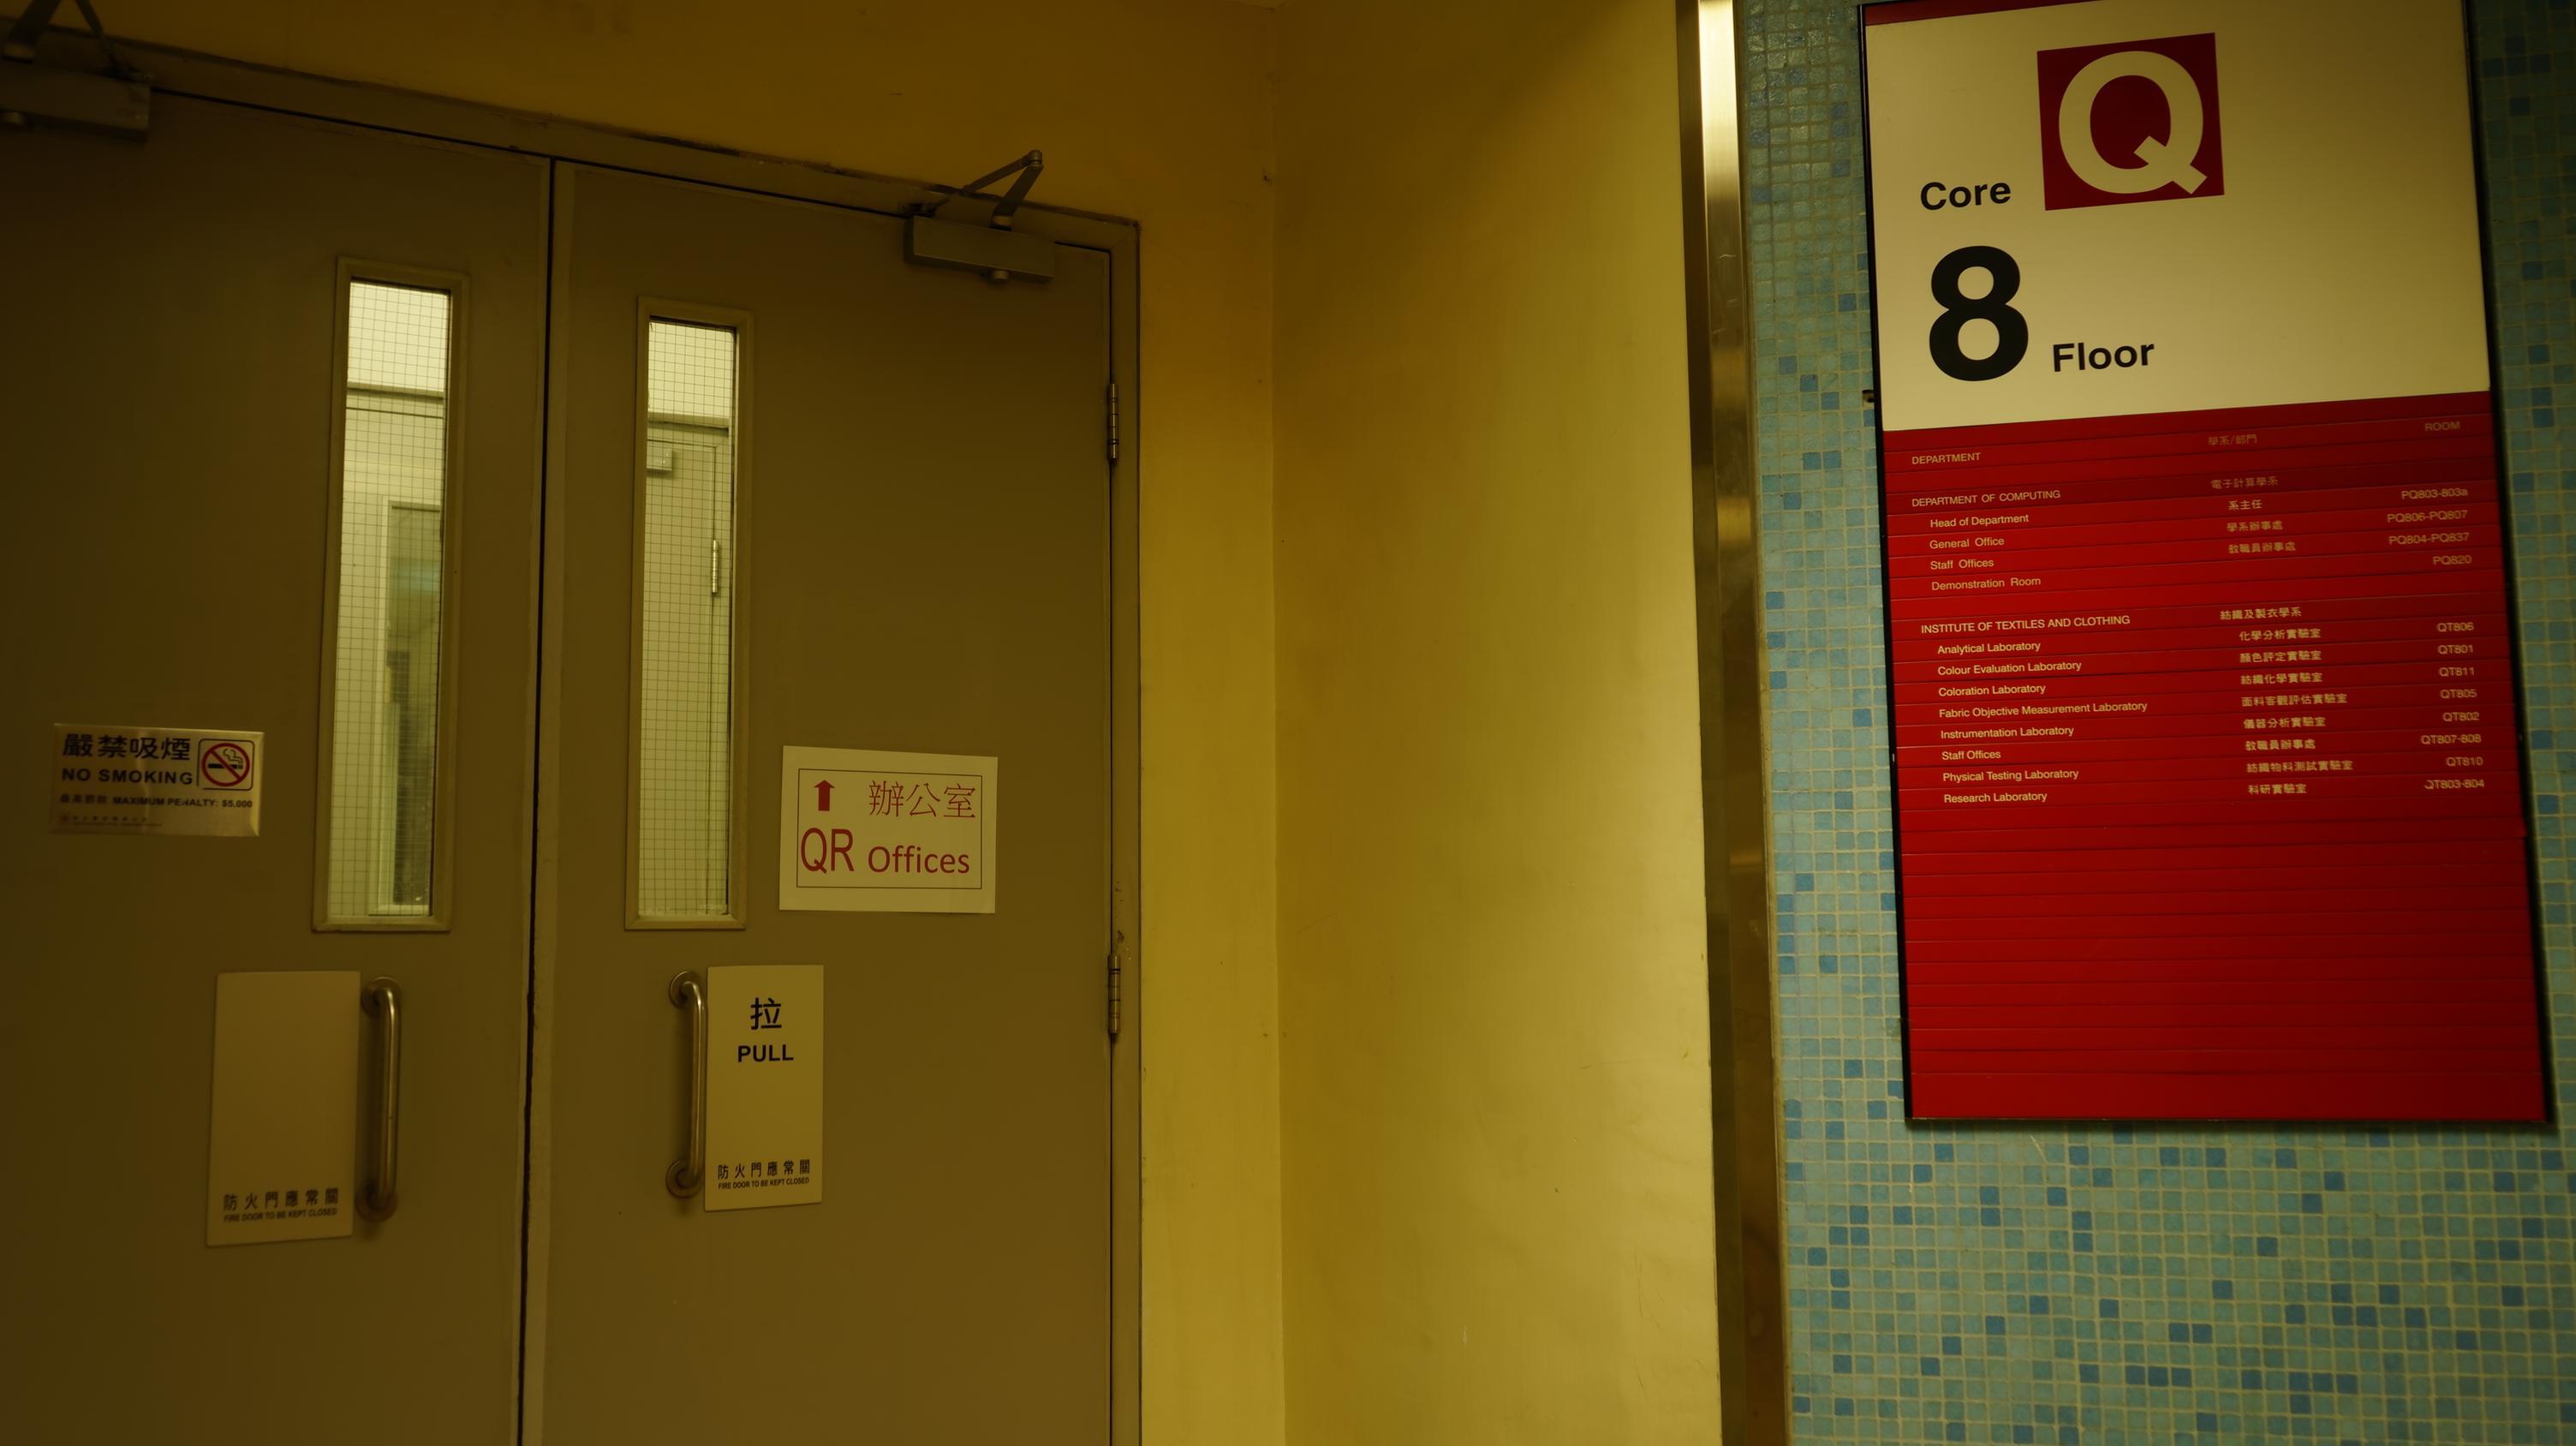
\includegraphics[width=1\textwidth]{images/dataset/Sony_4_200_3200_door_mean.JPG}}
\end{minipage}
\begin{minipage}[t]{0.4\textwidth}
\centering
\raisebox{-0.5cm}{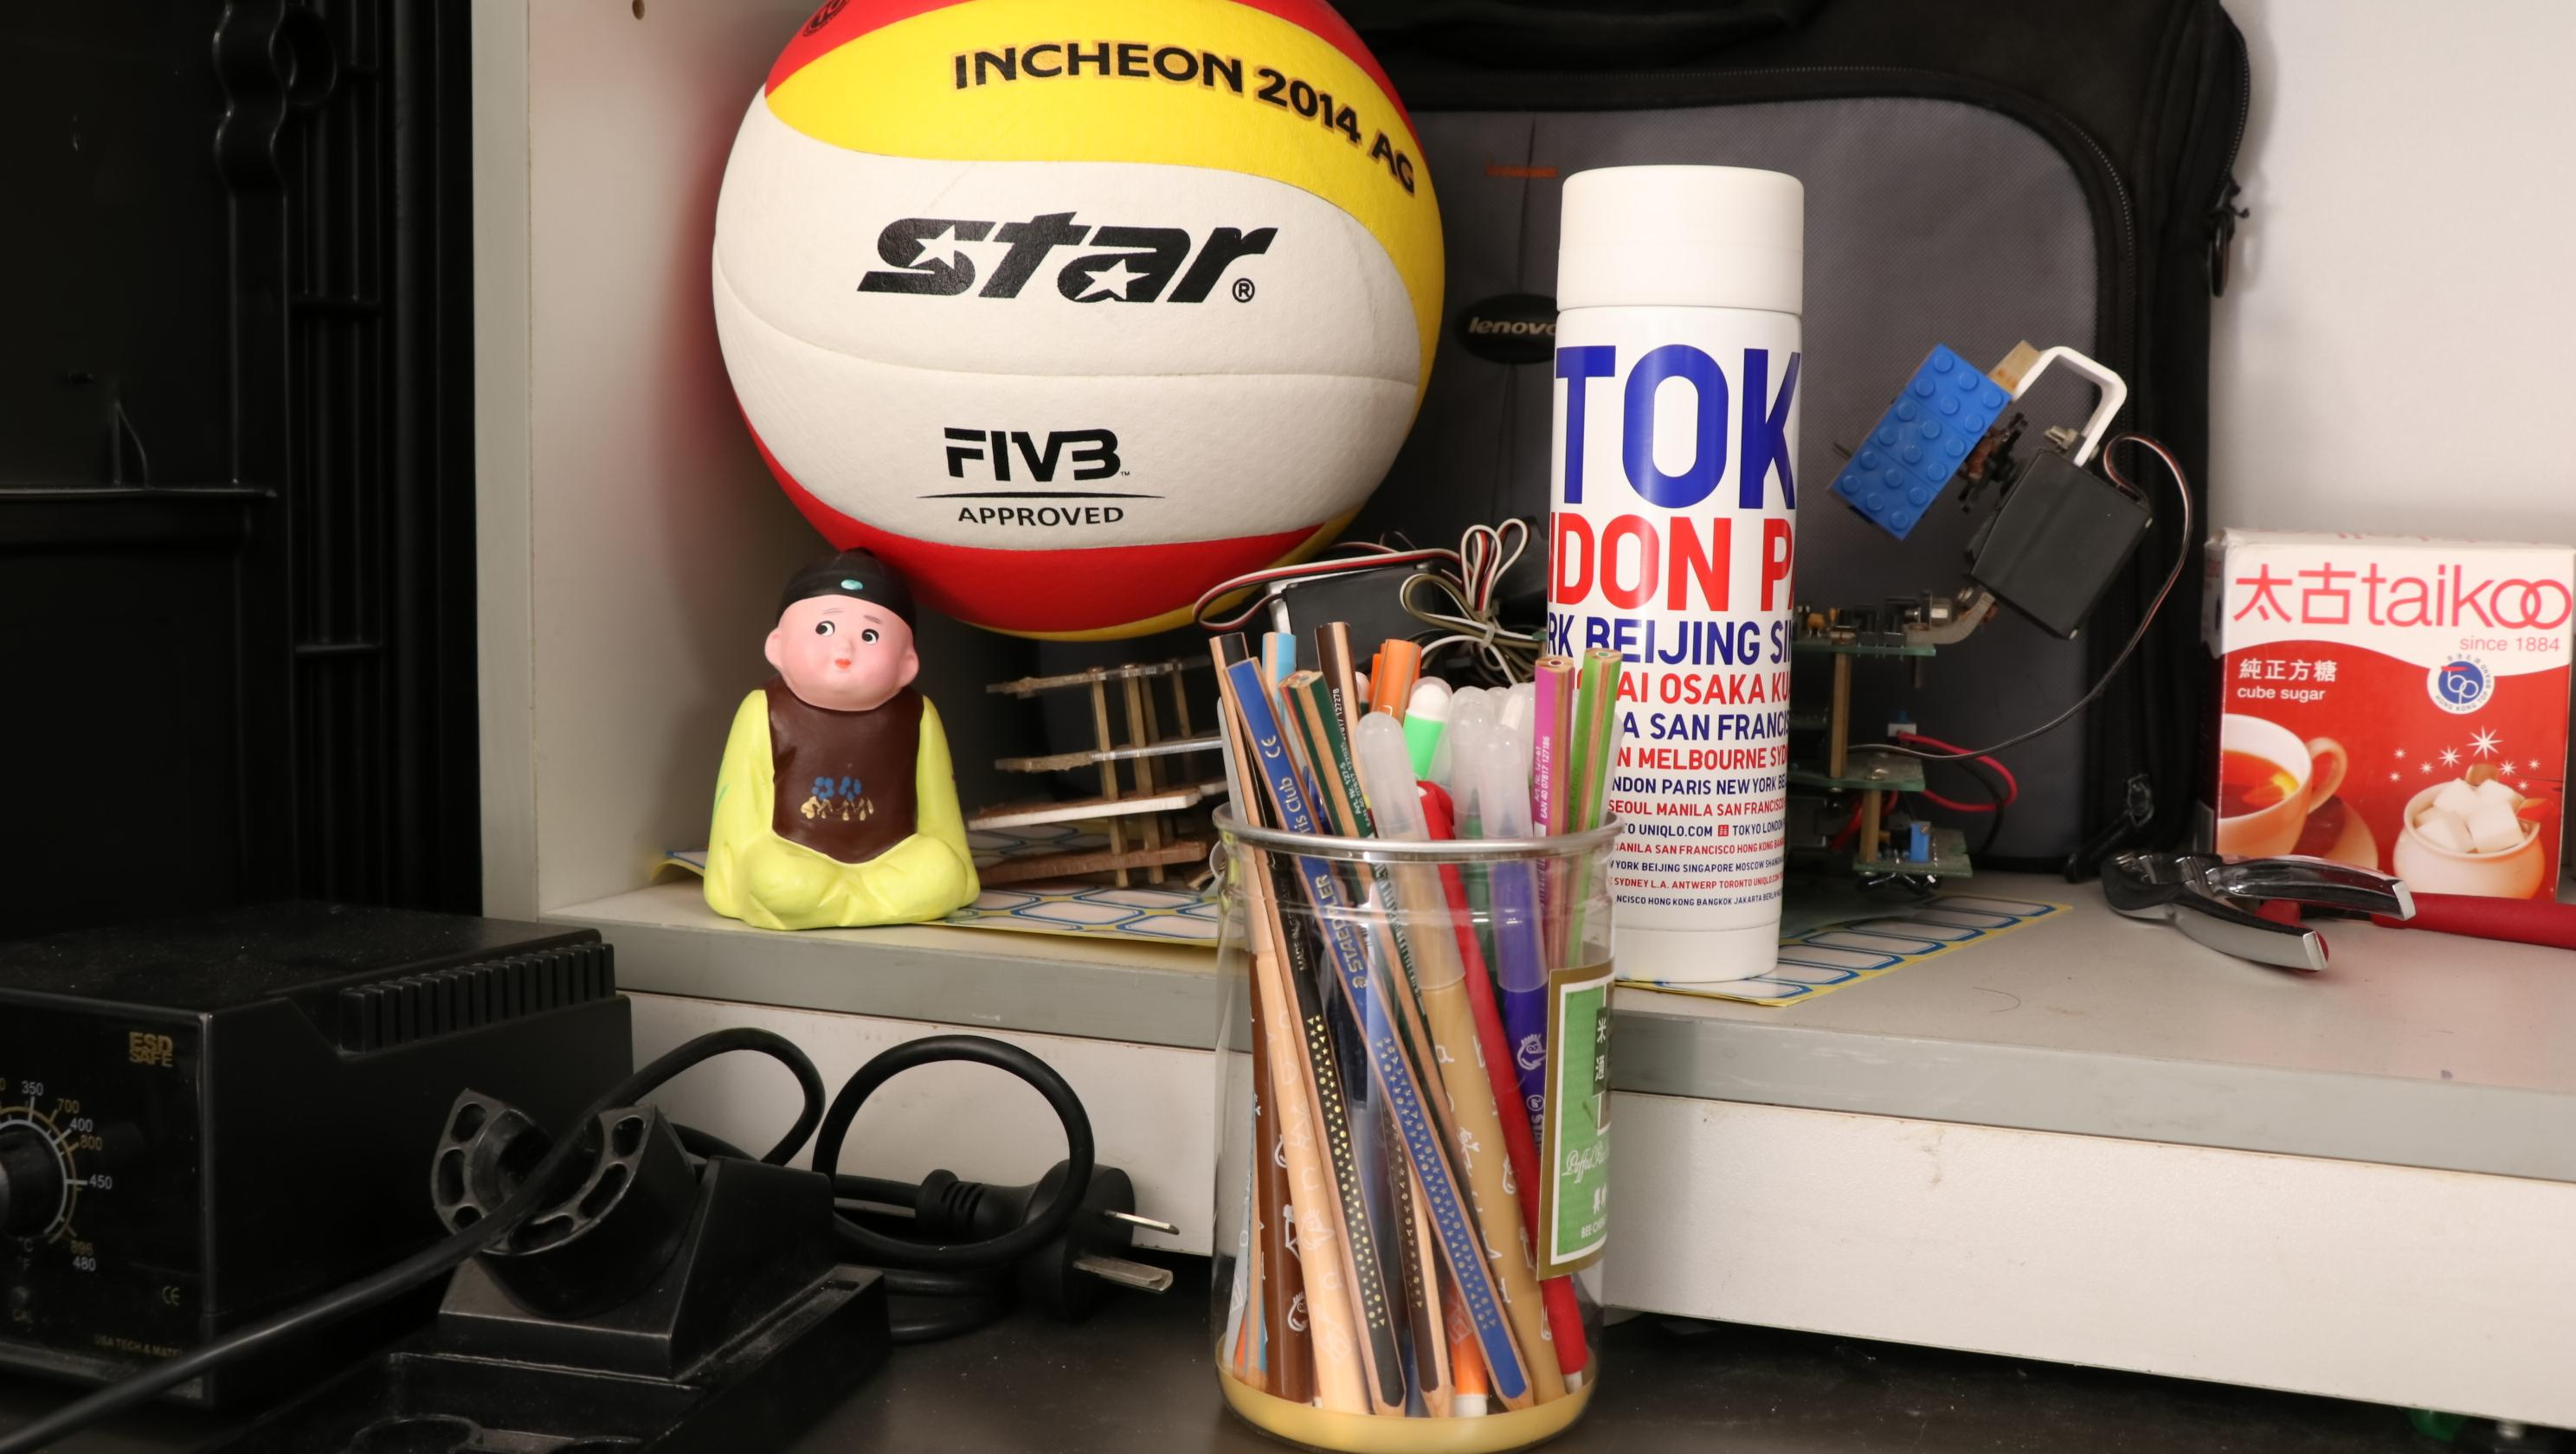
\includegraphics[width=1\textwidth]{images/dataset/Canon80D_8_8_3200_ball_mean.JPG}}
\end{minipage}
}\vspace{-3mm}
\subfigure{
\begin{minipage}[t]{0.4\textwidth}
\centering
\raisebox{-0.5cm}{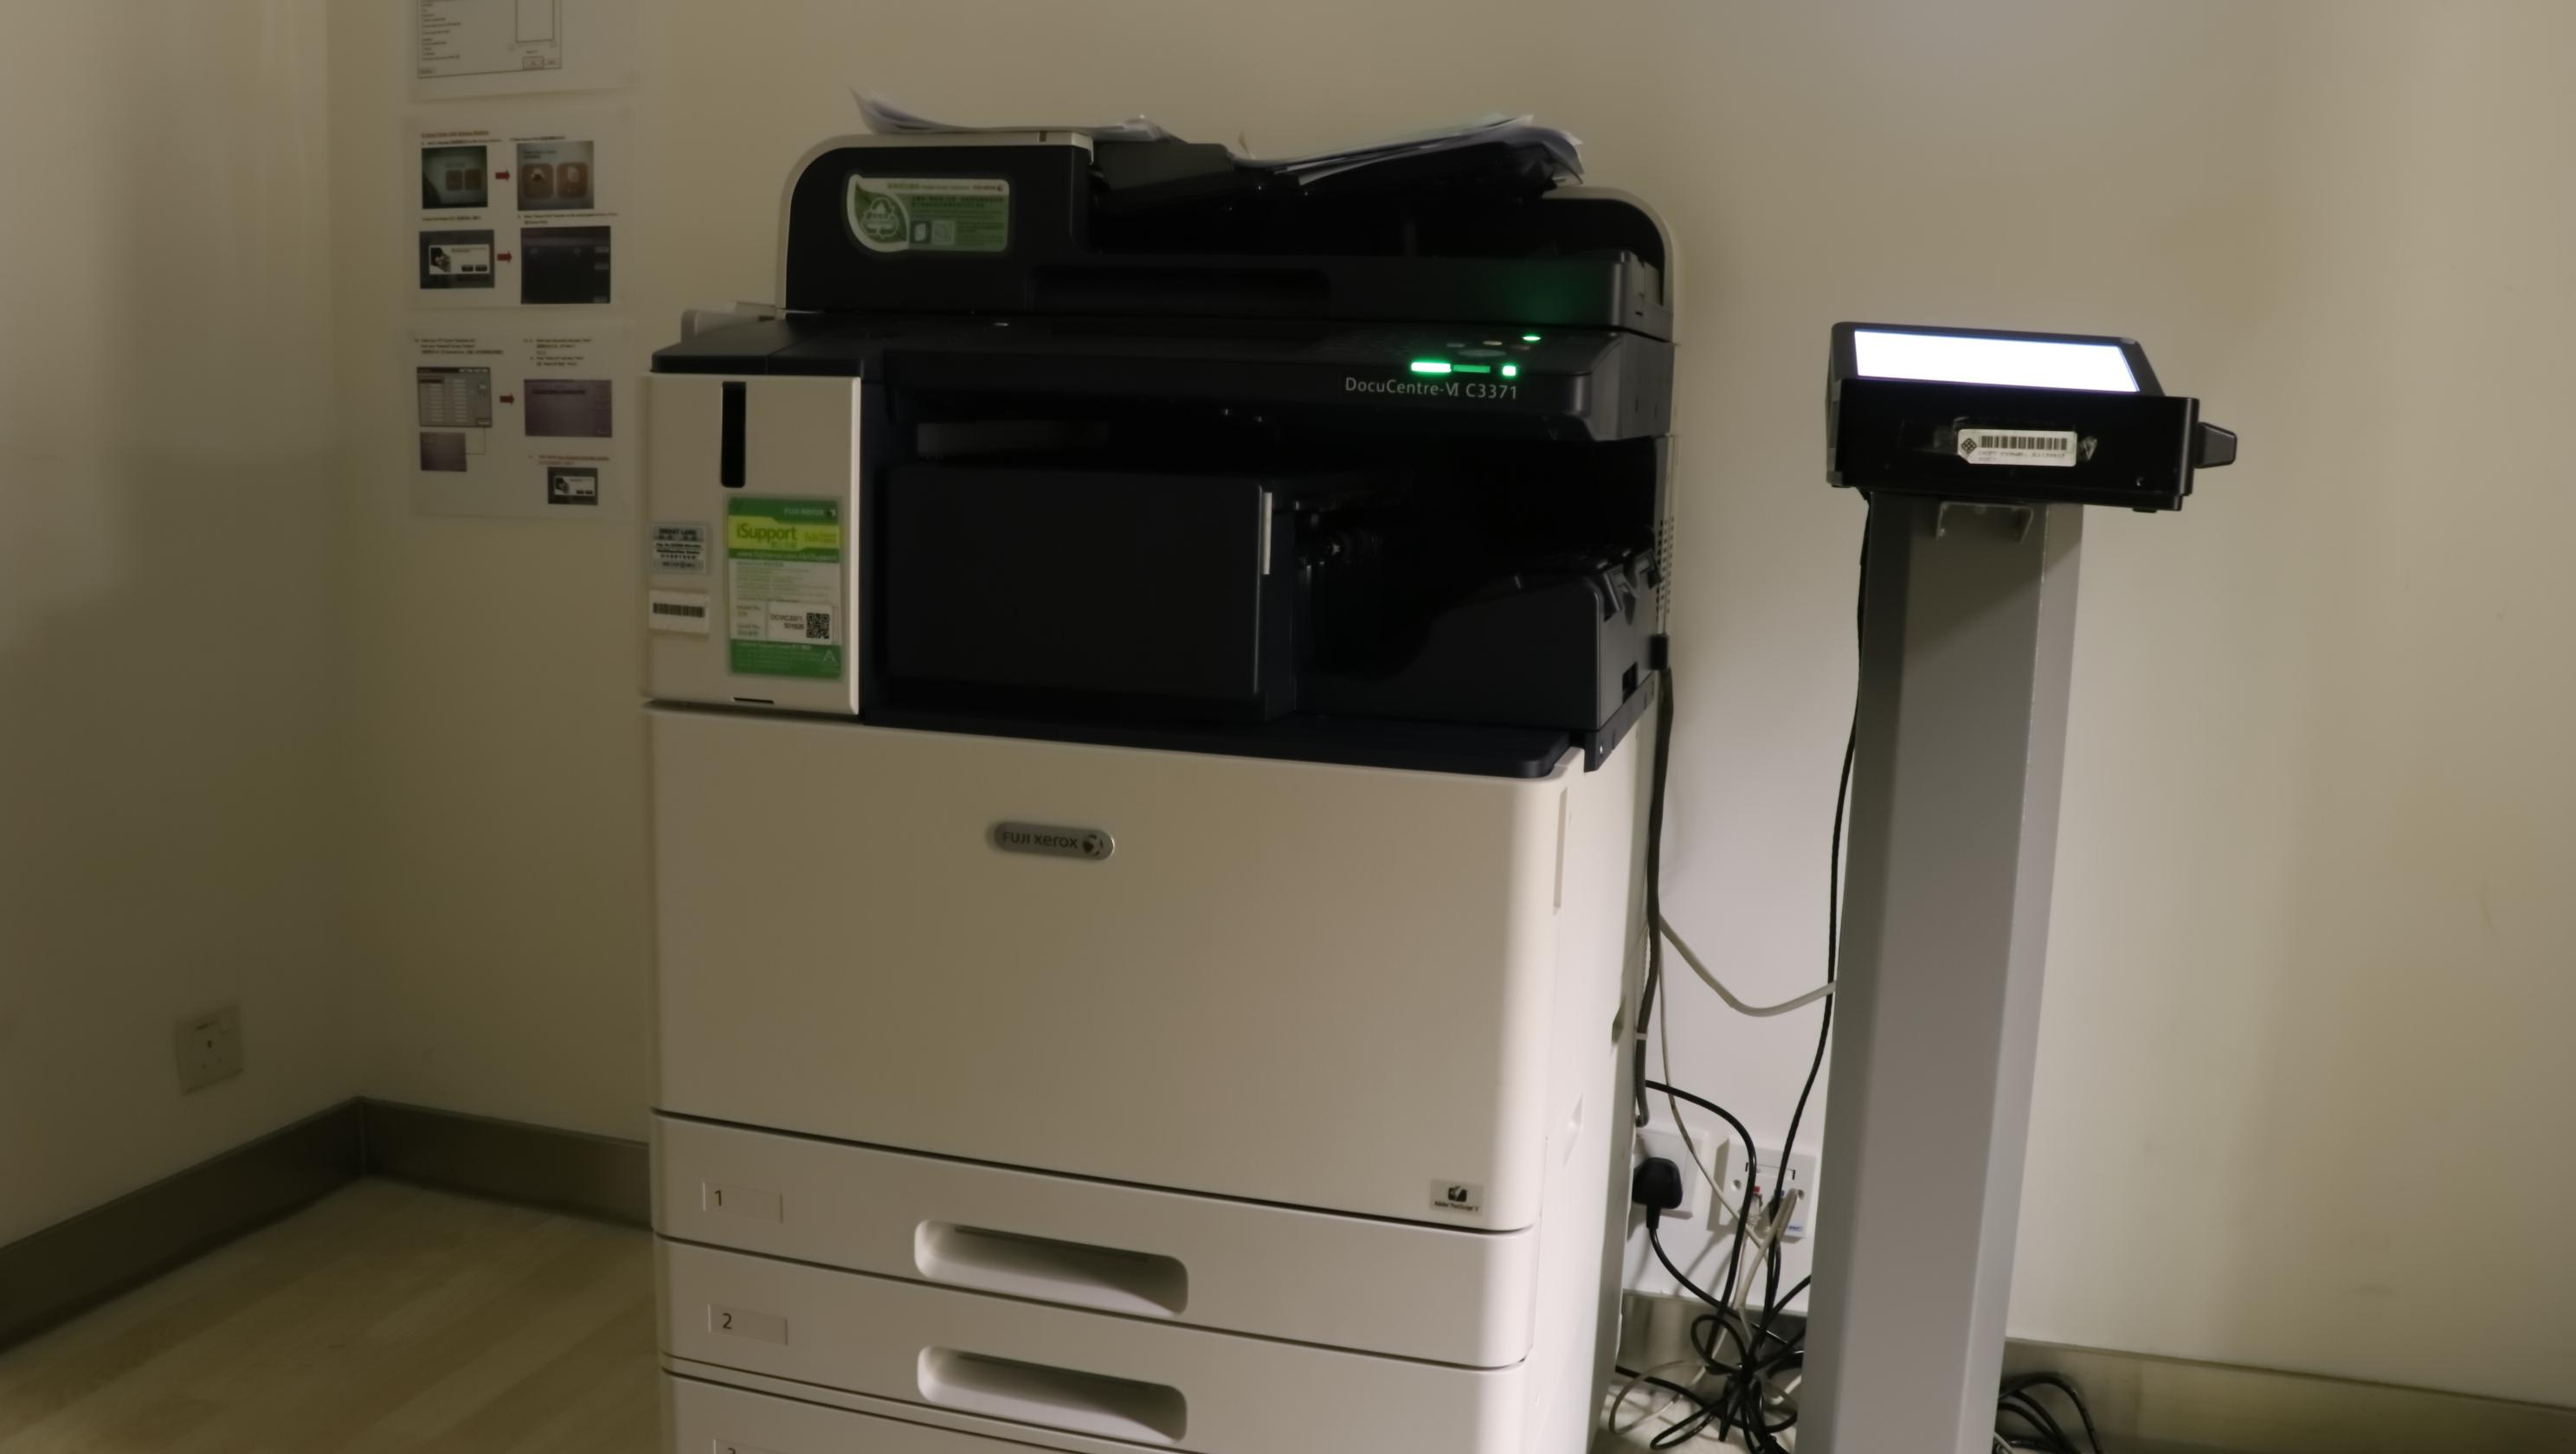
\includegraphics[width=1\textwidth]{images/dataset/Canon80D_8_8_12800_printer_mean.JPG}}
\end{minipage}
\begin{minipage}[t]{0.4\textwidth}
\centering
\raisebox{-0.5cm}{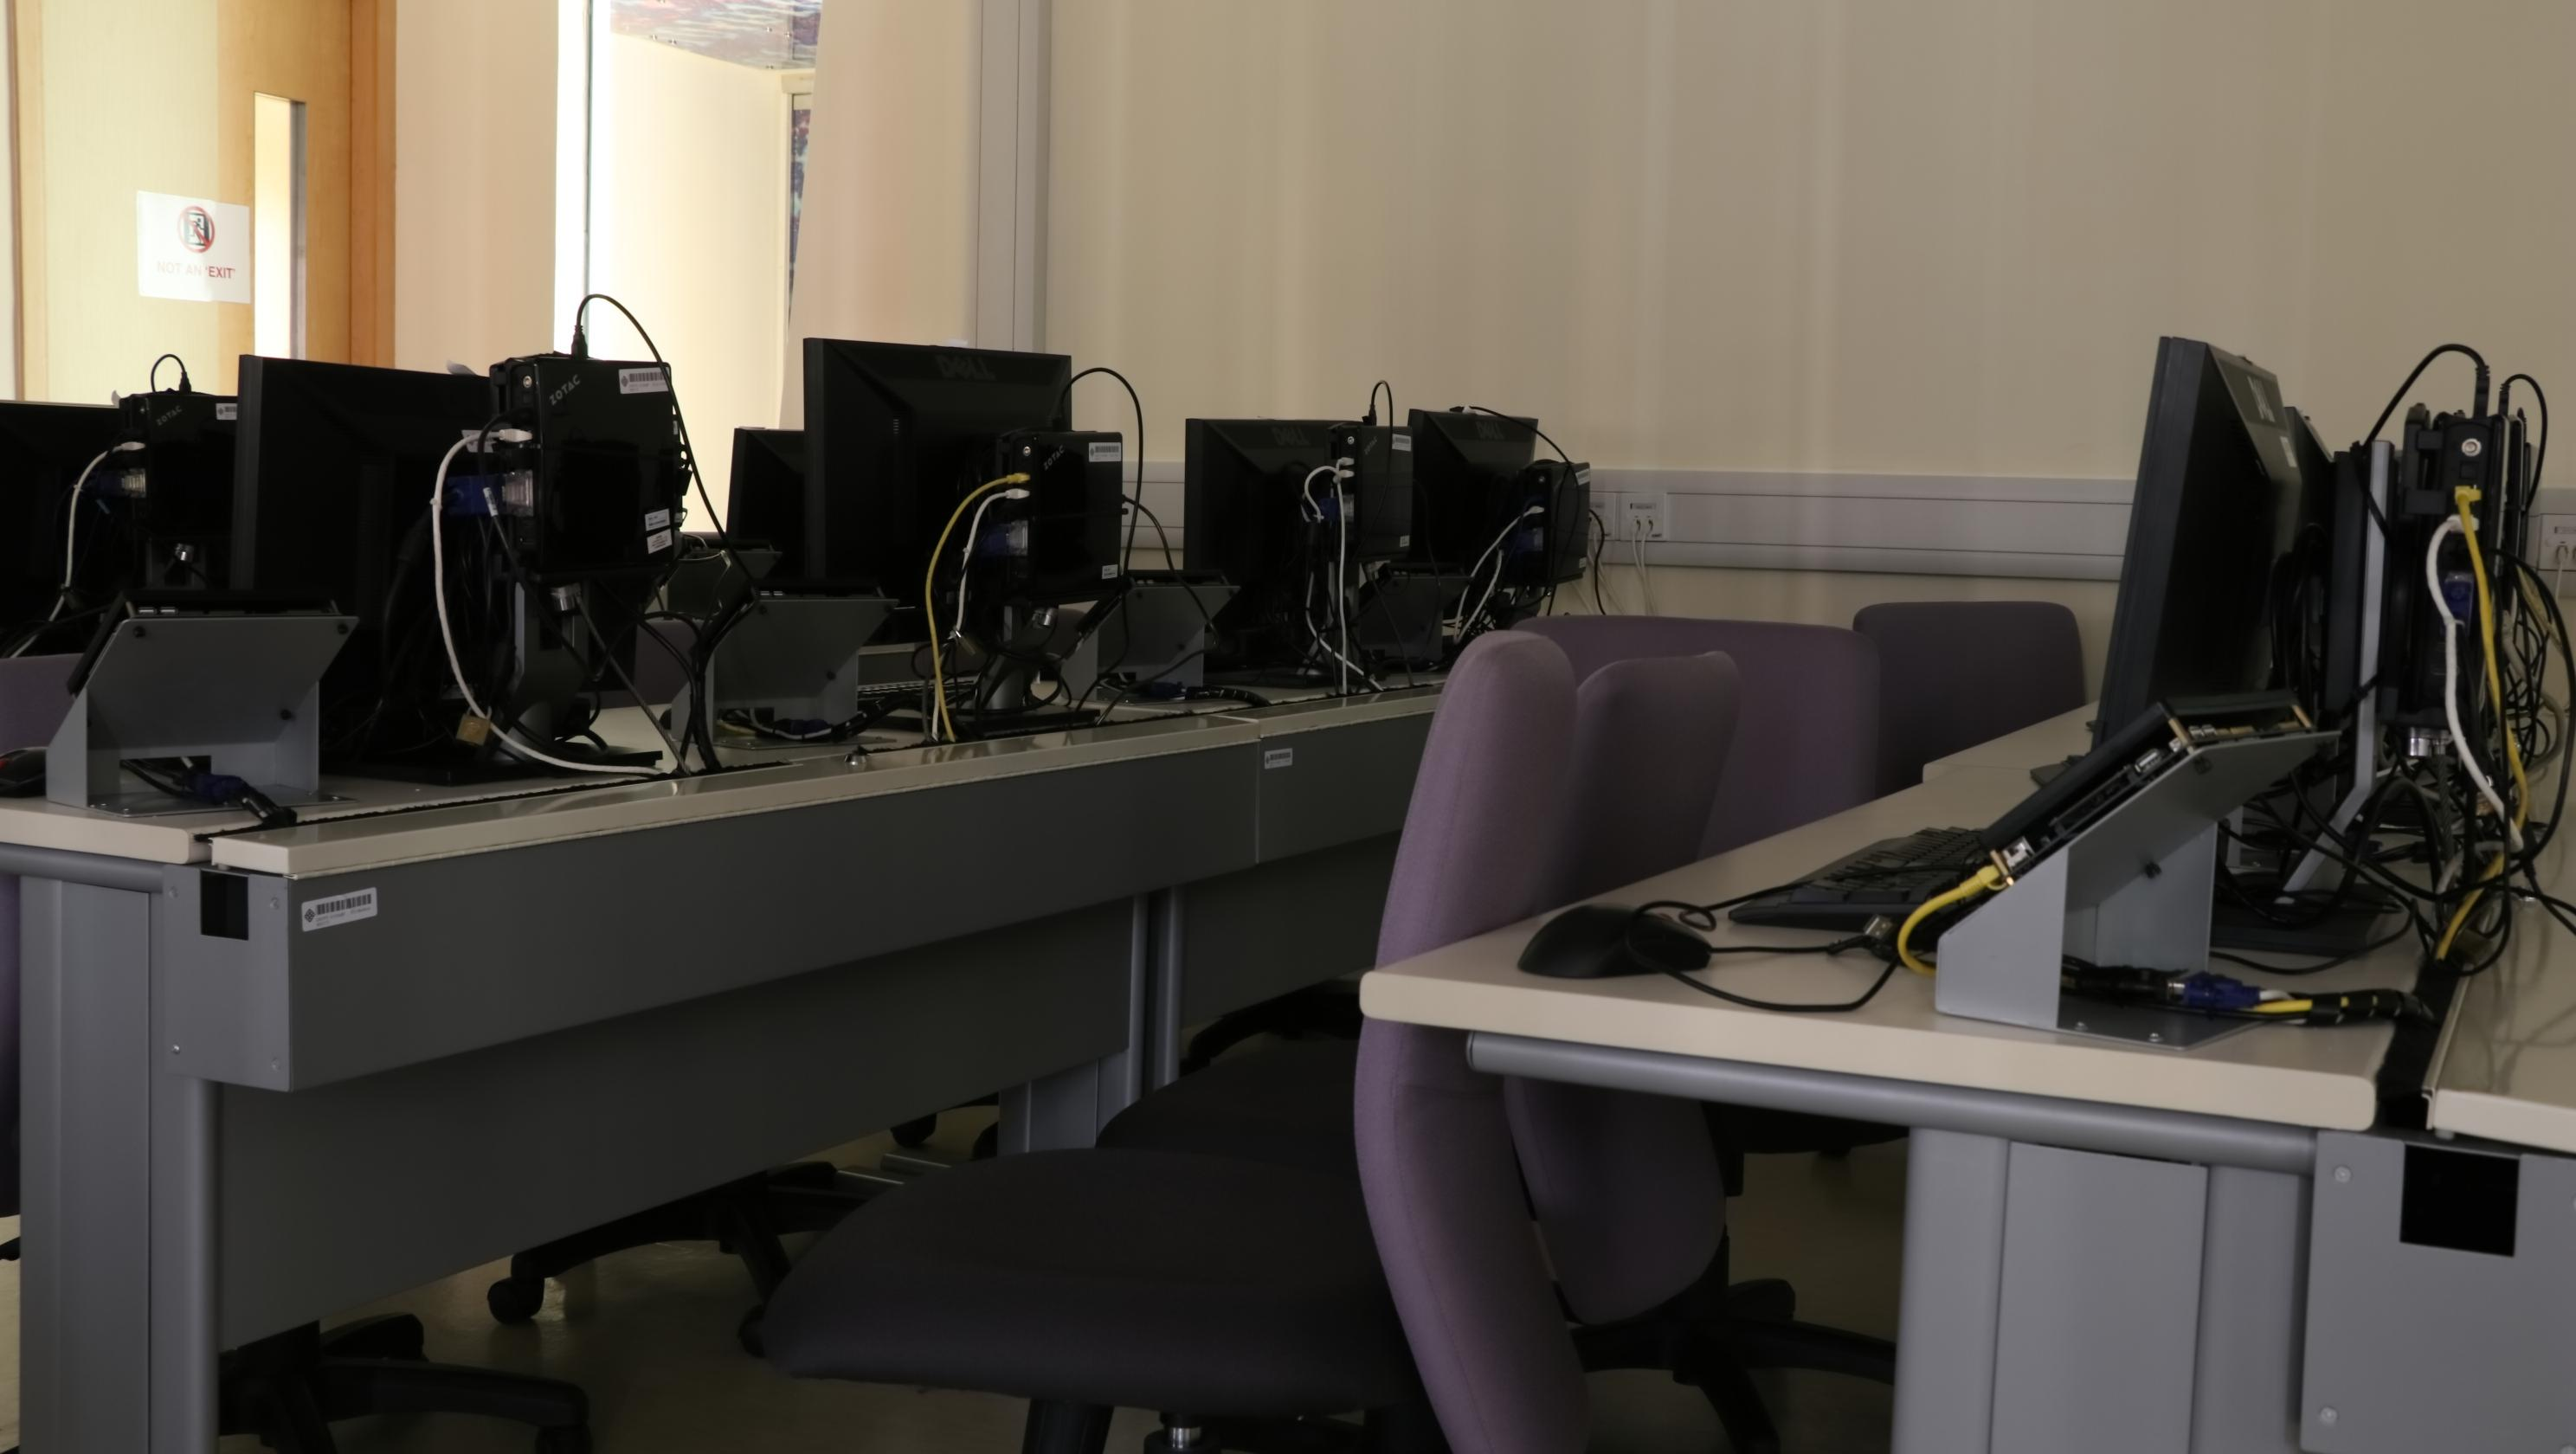
\includegraphics[width=1\textwidth]{images/dataset/Canon80D_8_8_6400_comproom_mean.JPG}}
\end{minipage}
}
\caption{Some examples in our newly constructed dataset.}
\label{fig6-3}
\end{figure}

\begin{figure}
\centering
\subfigure{
\begin{minipage}[t]{0.24\textwidth}
\centering
\raisebox{-0.5cm}{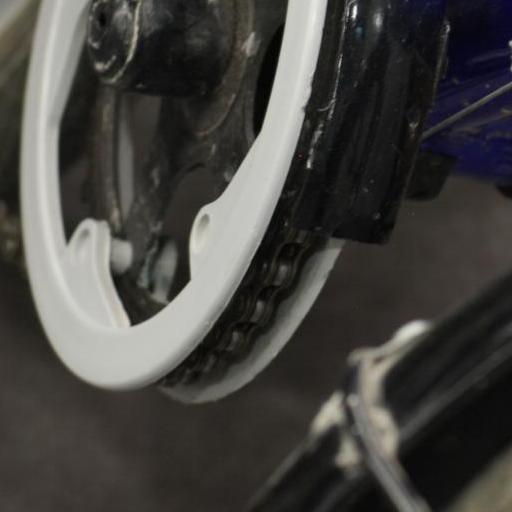
\includegraphics[width=1\textwidth]{images/dataset/Canon5D2_5_160_6400_bicycle_6_mean.JPG}}
\end{minipage}
\begin{minipage}[t]{0.24\textwidth}
\centering
\raisebox{-0.5cm}{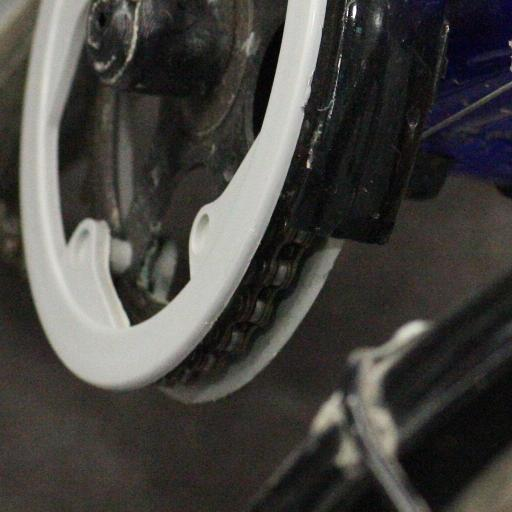
\includegraphics[width=1\textwidth]{images/dataset/Canon5D2_5_160_6400_bicycle_6_real.JPG}}
\end{minipage}
\begin{minipage}[t]{0.24\textwidth}
\centering
\raisebox{-0.5cm}{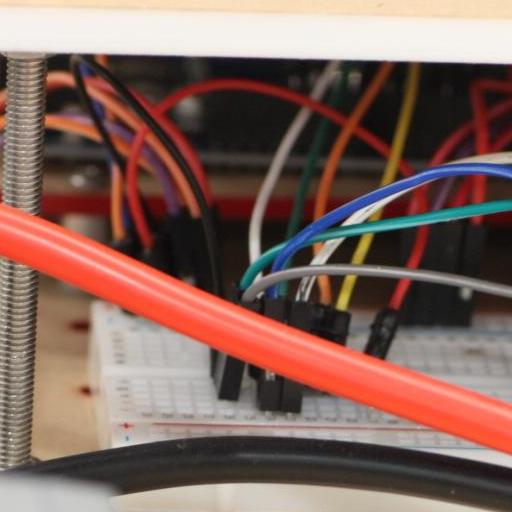
\includegraphics[width=1\textwidth]{images/dataset/Canon5D2_5_160_6400_circuit_11_mean.JPG}}
\end{minipage}
\begin{minipage}[t]{0.24\textwidth}
\centering
\raisebox{-0.5cm}{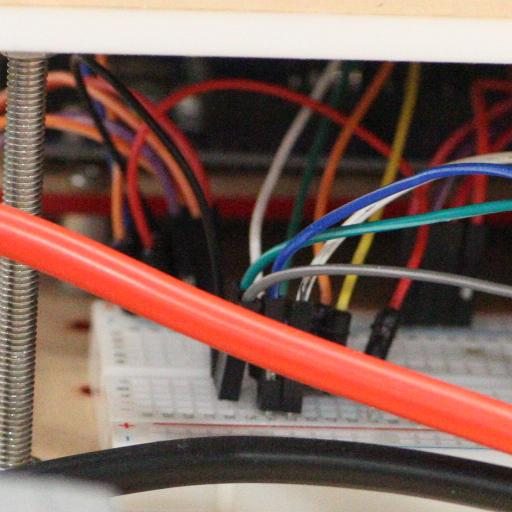
\includegraphics[width=1\textwidth]{images/dataset/Canon5D2_5_160_6400_circuit_11_real.JPG}}
\end{minipage}
}
\subfigure{
\begin{minipage}[t]{0.24\textwidth}
\centering
\raisebox{-0.5cm}{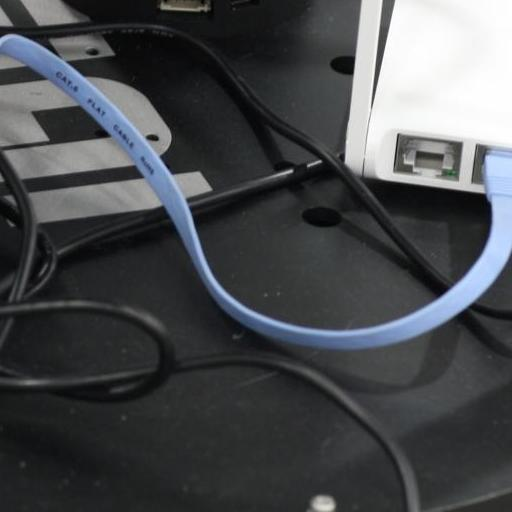
\includegraphics[width=1\textwidth]{images/dataset/Canon5D2_5_160_6400_reciever_1_mean.JPG}}
\end{minipage}
\begin{minipage}[t]{0.24\textwidth}
\centering
\raisebox{-0.5cm}{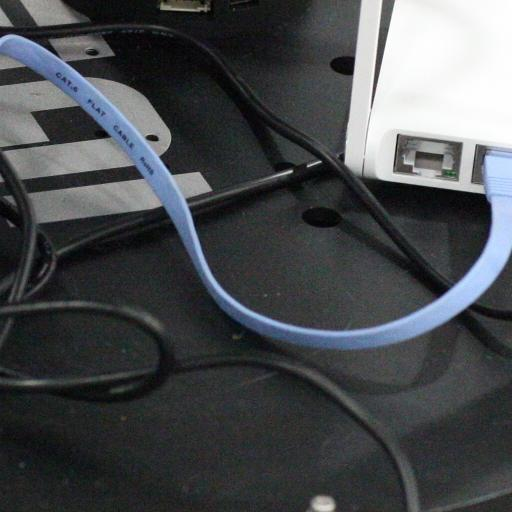
\includegraphics[width=1\textwidth]{images/dataset/Canon5D2_5_160_6400_reciever_1_real.JPG}}
\end{minipage}
\begin{minipage}[t]{0.24\textwidth}
\centering
\raisebox{-0.5cm}{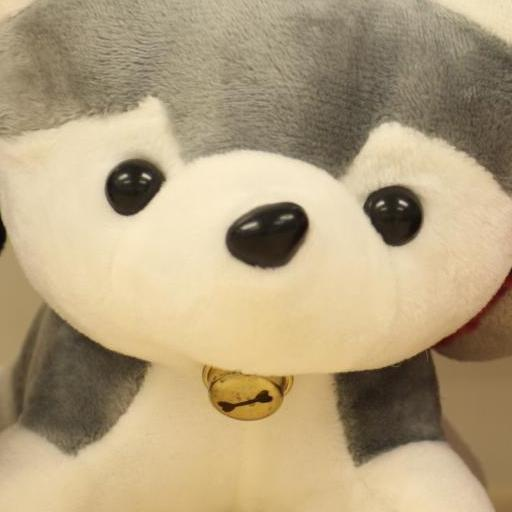
\includegraphics[width=1\textwidth]{images/dataset/Canon5D2_5_200_3200_toy_3_mean.JPG}}
\end{minipage}
\begin{minipage}[t]{0.24\textwidth}
\centering
\raisebox{-0.5cm}{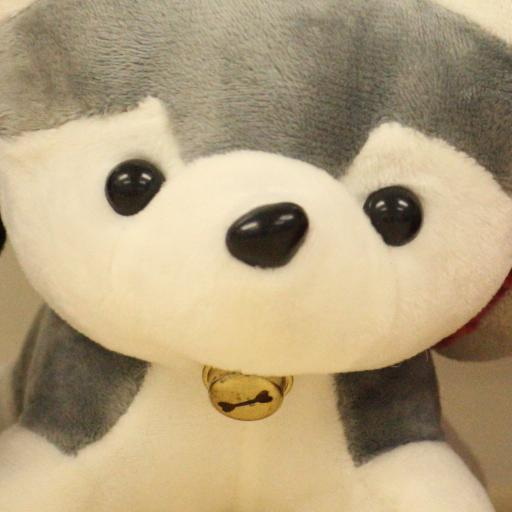
\includegraphics[width=1\textwidth]{images/dataset/Canon5D2_5_200_3200_toy_3_real.JPG}}
\end{minipage}
}
\subfigure{
\begin{minipage}[t]{0.24\textwidth}
\centering
\raisebox{-0.5cm}{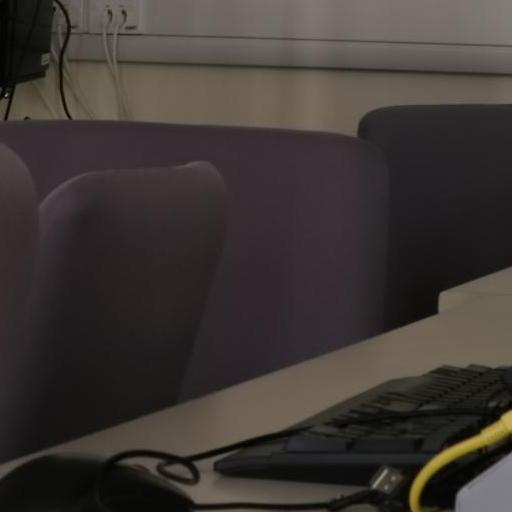
\includegraphics[width=1\textwidth]{images/dataset/Canon80D_8_8_6400_comproom_11_mean.JPG}}
\end{minipage}
\begin{minipage}[t]{0.24\textwidth}
\centering
\raisebox{-0.5cm}{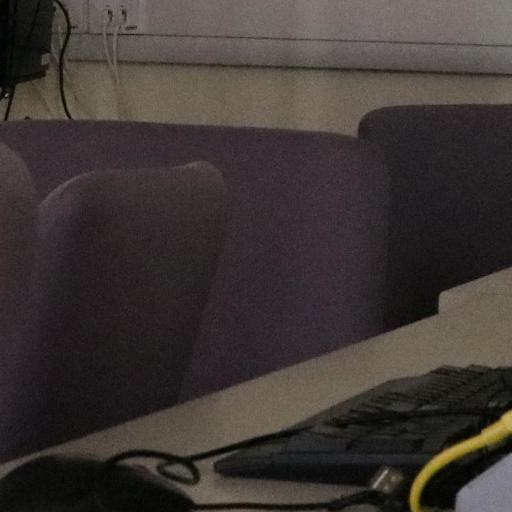
\includegraphics[width=1\textwidth]{images/dataset/Canon80D_8_8_6400_comproom_11_real.JPG}}
\end{minipage}
\begin{minipage}[t]{0.24\textwidth}
\centering
\raisebox{-0.5cm}{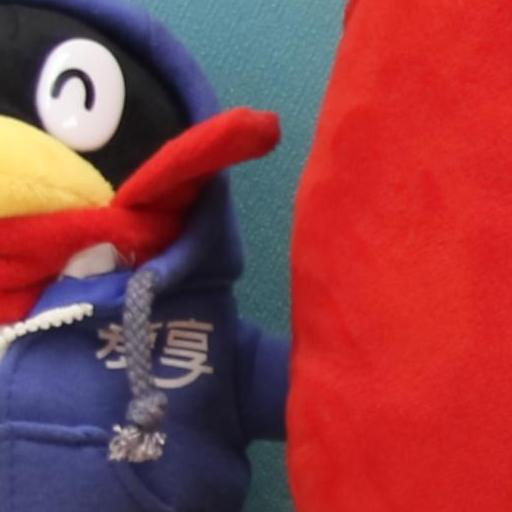
\includegraphics[width=1\textwidth]{images/dataset/Canon600D_4-5_125_1600_toy_16_mean.JPG}}
\end{minipage}
\begin{minipage}[t]{0.24\textwidth}
\centering
\raisebox{-0.5cm}{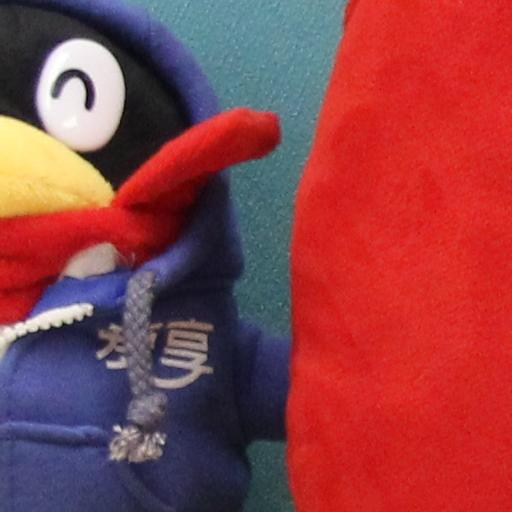
\includegraphics[width=1\textwidth]{images/dataset/Canon600D_4-5_125_1600_toy_16_real.JPG}}
\end{minipage}
}
\subfigure{
\begin{minipage}[t]{0.24\textwidth}
\centering
\raisebox{-0.5cm}{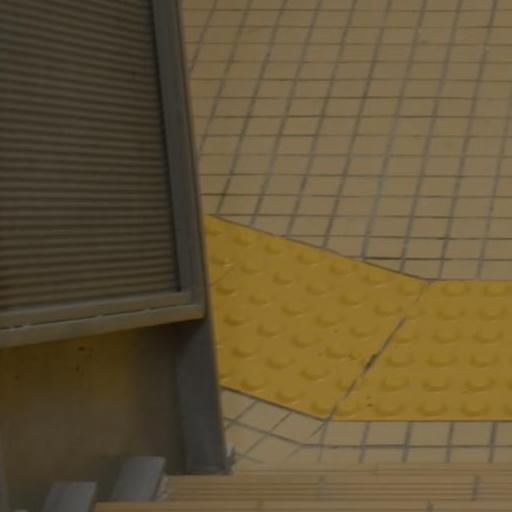
\includegraphics[width=1\textwidth]{images/dataset/NikonD800_5_125_6400_stair_3_mean.JPG}}
\end{minipage}
\begin{minipage}[t]{0.24\textwidth}
\centering
\raisebox{-0.5cm}{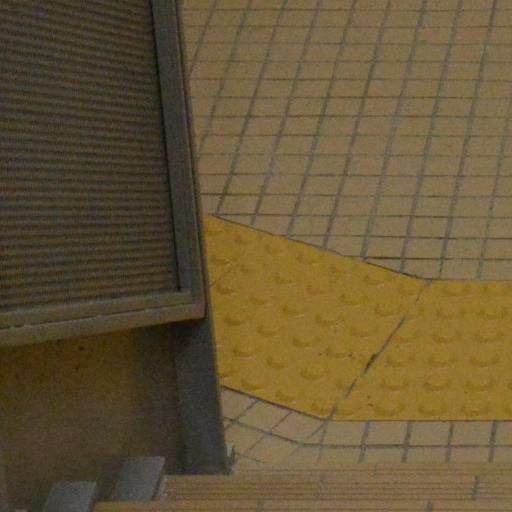
\includegraphics[width=1\textwidth]{images/dataset/NikonD800_5_125_6400_stair_3_real.JPG}}
\end{minipage}
\begin{minipage}[t]{0.24\textwidth}
\centering
\raisebox{-0.5cm}{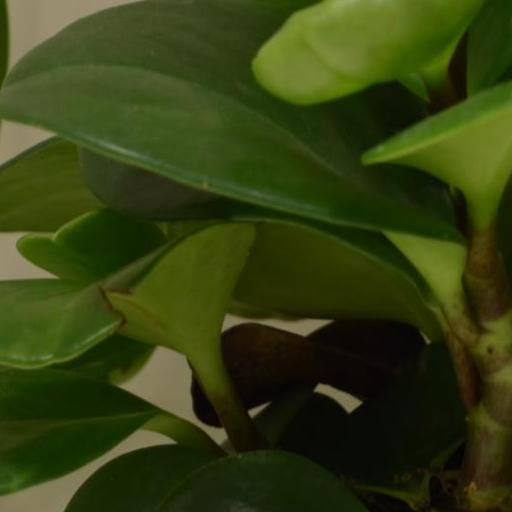
\includegraphics[width=1\textwidth]{images/dataset/NikonD800_6-3_125_5000_plant_1_mean.JPG}}
\end{minipage}
\begin{minipage}[t]{0.24\textwidth}
\centering
\raisebox{-0.5cm}{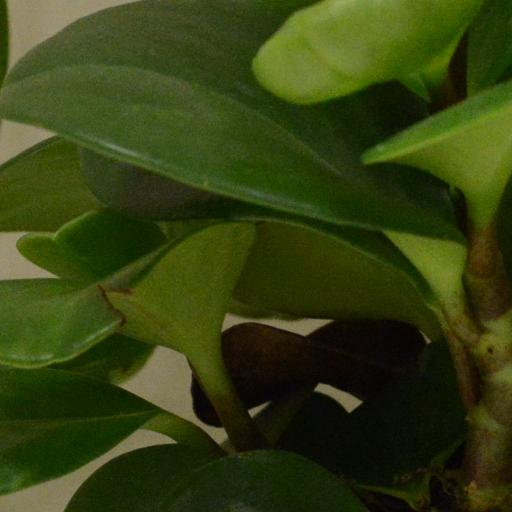
\includegraphics[width=1\textwidth]{images/dataset/NikonD800_6-3_125_5000_plant_1_real.JPG}}
\end{minipage}
}
\subfigure{
\begin{minipage}[t]{0.24\textwidth}
\centering
\raisebox{-0.5cm}{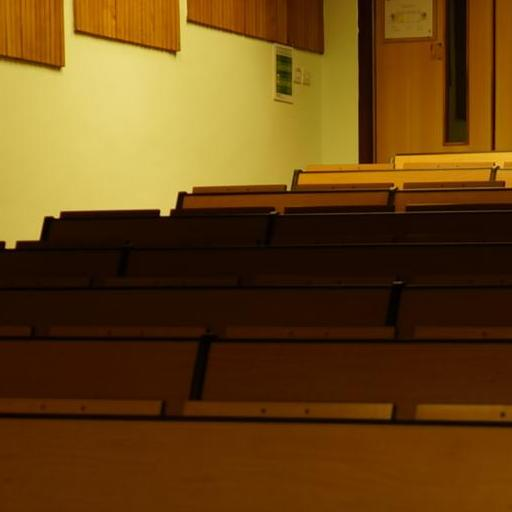
\includegraphics[width=1\textwidth]{images/dataset/Sony_3-5_200_1600_classroom_14_mean.JPG}}
\end{minipage}
\begin{minipage}[t]{0.24\textwidth}
\centering
\raisebox{-0.5cm}{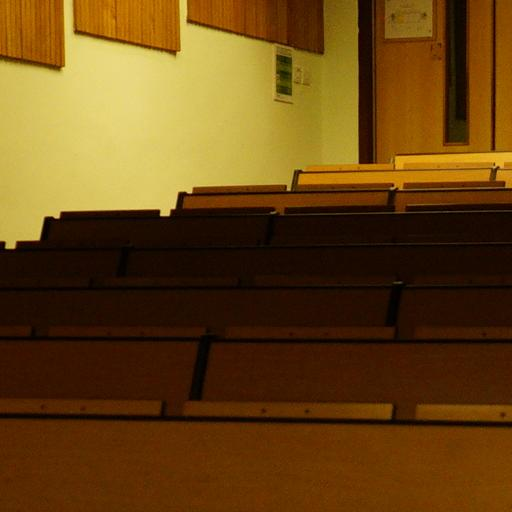
\includegraphics[width=1\textwidth]{images/dataset/Sony_3-5_200_1600_classroom_14_real.JPG}}
\end{minipage}
\begin{minipage}[t]{0.24\textwidth}
\centering
\raisebox{-0.5cm}{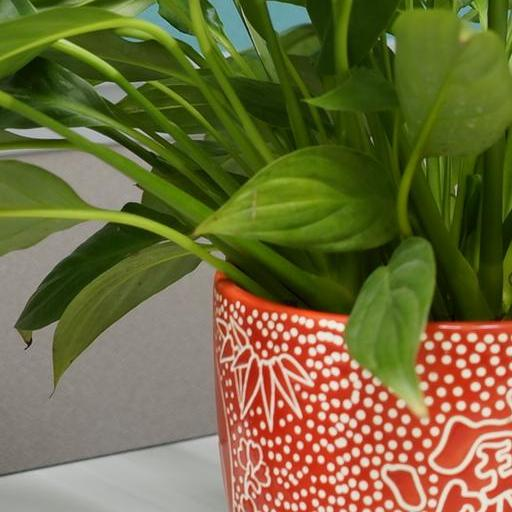
\includegraphics[width=1\textwidth]{images/dataset/Sony_4-5_125_3200_plant_10_mean.JPG}}
\end{minipage}
\begin{minipage}[t]{0.24\textwidth}
\centering
\raisebox{-0.5cm}{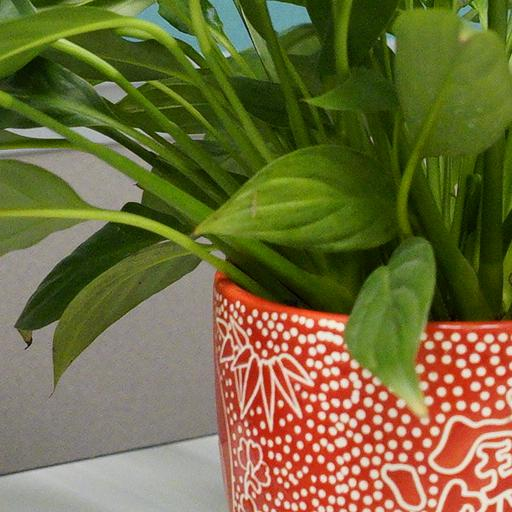
\includegraphics[width=1\textwidth]{images/dataset/Sony_4-5_125_3200_plant_10_real.JPG}}
\end{minipage}
}
    \caption{Some cropped parts of the ``ground truth'' images (up) and their corresponding realistic images (down) in our newly constructed dataset.}
    \label{fig6-4}
\end{figure}


Since the images we captured are very large, we crop 100 smaller regions from the 40 scenes to evaluated the existing image denoising methods. Some examples of the cropped regions and their corresponding ``ground truth'' images are listed in Figure \ref{fig6-4}. Besides, one can see that the ``ground truth'' image contains much less noise than the noisy image and has much better visual quality. Hence, this dataset provide us a good platform for evaluating the image denoising methods. The detailed description on cameras and camera settings is listed in Table \ref{tab6-4}. One can see that in our dataset, the ISO values are more comprehensive than the previous datasets \cite{RENOIR2014,crosschannel2016,dnd2017}. For better evaluation of image denoising methods, we crop 100 regions as our final testing set.

\begin{table}[t!]
\caption{Cameras and camera settings used in our new dataset.}
\label{tab6-4}
\begin{center}
\small
\renewcommand\arraystretch{1.2}
\begin{tabular*}{1\textwidth}{@{\extracolsep{\fill}}ccccc}
\hline
Camera
&
\# Scene
&
Sensor size (mm)
&
\# Image
&
ISO
\\
\hline
Canon 5D & 10  & $36\times24$  & 29  & 3.2k,6.4k
\\
\hline
Canon 80D & 6  & $22.5\times15$  & 15 & 800,1.6k,3.2k,6.4k,12.8k 
\\
\hline   
Canon 600D & 5 & $22.3\times14.9$  & 11  & 1.6k,3.2k 
\\
\hline   
Nikon D800 & 12 & $35.9\times24$  & 33 & 1.6k,1.8k,3.2k,5k,6.4k 
\\
\hline   
Sony A7II & 7 & $35.8\times23.9$  & 12  & 1.6k,3.2k,6.4k 
\\
\hline
\end{tabular*}
\end{center}
\vspace{-5mm}
\end{table}

\section{Experiments}

\subsection{Benchmark Datasets} 

To better illustrate the effectiveness of existing image denising methods, we apply the competing methods on existing datasets \cite{crosschannel2016,dnd2017} and our proposed new dataset, which contains overall 100 test images. These images share very small (less than $10\%$) overlap at contents. Since the captured real-world noisy images in \cite{RENOIR2014} have clear color difference with corresponding ``ground truth'' images, we do not evaluate the existing image denoising methods on this dataset.

\textbf{Dataset 1} is provided in \cite{crosschannel2016}, which includes noisy images of 11 static scenes captured by Canon 5D Mark 3, Nikon D600, and Nikon D800 cameras.\ 15 regions of size $512\times512$ were cropped to evaluate the different denoising methods.  

\textbf{Dataset 2} is called the Darmstadt Noise Dataset (DND) \cite{dnd2017}, which includes 50 different pairs of images of the same scenes captured by Sony A7R, Olympus E-M10, Sony RX100 IV, and Huawei Nexus 6P.\ The authors cropped 20 bounding boxes of $512\times512$ pixels from each image in the dataset, yielding 1000 test crops in total.\ However, the ``ground truth'' images are not open access, and we can only submit the denoising results to the authors' \href{https://noise.visinf.tu-darmstadt.de/}{Project Website} and get the PSNR and SSIM \cite{ssim} results.

\textbf{Dataset 3} is our constructed dataset, which includes noisy images of 40 static scenes captured by Canon 5D Mark II, Canon 80D, Canon 600D, Nikon D800, and Sony A7 II cameras.\ 100 regions of size $512\times512$ were cropped to evaluate the different denoising methods.

\subsection{Comparison Methods}

With the proposed dataset, we make a comprehensive evaluation on the state-of-the-art image denoising methods, including the famous CBM3D \cite{cbm3d}, Expected Patch Log Likelihood (EPLL) \cite{epll}, multi-layer perception (MLP) \cite{mlp}, Nonlocally Centralized Sparse Representations (NCSR) \cite{ncsr}, Cascades of Shrinkage Fileds (CSF) \cite{csf}, Weighted Nuclear Norm Minimization (WNNM) \cite{wnnm}, Trainable Nonlinear Reactive Diffusion (TNRD) \cite{tnrd}, the residual network based method DnCNN \cite{dncnn}, the ``Noise Clinic'' method \cite{noiseclinic,ncwebsite}, the commercial software Neat Image \cite{neatimage}, and our proposed methods Patch Group Prior based Denoising (PGPD) \cite{pgpd}, external prior guided internal prior learning for image denoising (Guided) \cite{guided}, Multi-channel Weighted Nuclear Norm Minimization (MCWNNM) \cite{mcwnnm}, the Trilateral Weighted Sparse Coding (TWSC) \cite{twsc}. CBM3D is a state-of-the-art color image denoising method, which assumes that the noise is addtive white Gaussian nosie (AWGN). The EPLL, NCSR, CSF, WNNM, TNRD, DnCNN are state-of-the-art methods for AWGN noise removal on greyscale images, and we apply these methods on each channel of the realsitic color images.  The ``Noise Clnic'' (NC) is a blind image denoising method while Neat Image (NI) is a set of commercial software for image denoising, which has been embedded into Photoshop and Corel Paint Shop. Besides, the method of DnCNN \cite{dncnn} can also deal with real-world noisy images. Our proposed methods includes PGPD, Guided, MCWNNM, and TWSC. The PGPD is proposed for AWGN noise, while the Guided, MCWNNM, and TWSC are proposed for real-world noisy image denoising.

\textbf{Noise level of comparison methods.} For the CBM3D method, the standard deviation of noise on color images should be given as a parameter. For methods of NCSR,  WNNM, MLP, CSF, and TNRD, the noise level in each color channel should be input. For the DnCNN method, it is trained to deal with noise in a range of levels $0\sim55$. We retrain the models of discriminative denoising methods MLP, CSF, and TNRD (using the released codes by the authors) at different noise levels from $\sigma=5$ to $\sigma=50$ with a gap of 5. The denoising is performed by processing each channel with the model trained at the same (or nearest) noise level. The noise levels ($\sigma_{r}, \sigma_{g}, \sigma_{b}$) in R, G, B channels are assumed to be Gaussian and can be estimated via some noise estimation methods \cite{noiselevel,Chen2015ICCV}. In this chapter, we employ the method \cite{noiselevel} to estimate the noise level for each color channel.


\subsection{Results and Discussion}

\textbf{Results on Dataset 1}. The average PSNR and SSIM results on the 15 cropped images by competing methods are listed in Table \ref{tab6-6}.\ One can see that the TWSC method performs much better than other competing methods.\ Figure\ \ref{fig6-5} shows the denoised images of a scene captured by Nikon D800 at ISO = 6400.\ One can see that the proposed TWSC method results in not only higher PSNR and SSIM measures, but also much better visual quality than other methods.\ More visual comparisons can be found in the supplementary file.

\begin{table}[t!]
\caption{Average results on PSNR(dB) and SSIM of different denoising algorithms on the 15 cropped images in \textbf{Dataset 1} \cite{crosschannel2016}.}
\scriptsize
\label{tab6-6}
\begin{center}
\renewcommand\arraystretch{1.2}
\begin{tabular*}{1\textwidth}{@{\extracolsep{\fill}}cccccccc}
\hline
Metric
&
\textbf{CBM3D}
&
\textbf{EPLL}
&
\textbf{NCSR}
&
\textbf{WNNM}
&
\textbf{MLP}
&
\textbf{CSF}
&
\textbf{TNRD}
\\
\hline
PSNR & 35.19  & 33.66 & 33.46 &  35.77 &  36.46 & 35.33 & 36.61  
\\
\hline
SSIM & 0.8580 & 0.8591  & 0.8512 & 0.9381 &  0.9436  & 0.9250 & 0.9463 
\\
\hline
Metric
&
\textbf{DnCNN}
&
\textbf{NC}
&
\textbf{NI}
&
\textbf{PGPD}
&
\textbf{Guided}
&
\textbf{MCWNNM}
&
\textbf{TWSC}
\\
\hline
PSNR &  33.86  & 36.43  & 35.49  & 33.69  &  37.15 &  37.71 &  \textbf{37.81}
\\
\hline
SSIM & 0.8635  &  0.9364 & 0.9126  & 0.8591  & 0.9504 &  0.9542 & \textbf{0.9586}
\\
\hline
\end{tabular*}
\end{center}
\end{table}

\begin{figure}[t!]
    \centering
\subfigure{
\begin{minipage}[t]{0.24\textwidth}
\centering
\raisebox{-0.5cm}{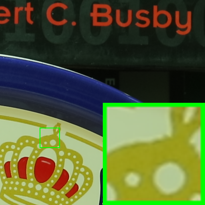
\includegraphics[width=1\textwidth]{images/dataset/cc/resize_br_Mean_5dmark3_iso3200_1_real.png}}
{\footnotesize Mean Image}
\end{minipage}
\begin{minipage}[t]{0.24\textwidth}
\centering
\raisebox{-0.5cm}{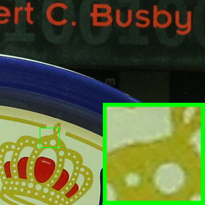
\includegraphics[width=1\textwidth]{images/dataset/cc/resize_br_Noisy_5dmark3_iso3200_1_real.png}}
{\footnotesize Noisy 37.00/0.9345}
\end{minipage}
\begin{minipage}[t]{0.24\textwidth}
\centering
\raisebox{-0.5cm}{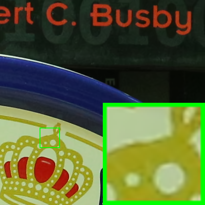
\includegraphics[width=1\textwidth]{images/dataset/cc/resize_br_CBM3D_5dmark3_iso3200_1_real.png}}
{\footnotesize CBM3D 39.72/0.9769}
\end{minipage}
\begin{minipage}[t]{0.24\textwidth}
\centering
\raisebox{-0.5cm}{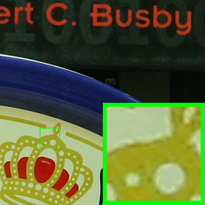
\includegraphics[width=1\textwidth]{images/dataset/cc/resize_br_EPLL_5dmark3_iso3200_1_real.png}}
{\footnotesize EPLL 37.61/0.9521}
\end{minipage}
}\vspace{-3mm}
\subfigure{
\begin{minipage}[t]{0.24\textwidth}
\centering
\raisebox{-0.5cm}{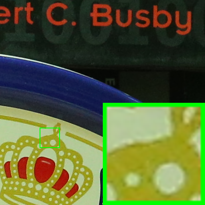
\includegraphics[width=1\textwidth]{images/dataset/cc/resize_br_NCSR_5dmark3_iso3200_1_real.png}}
{\footnotesize NCSR 37.93/0.9579}
\end{minipage}
\begin{minipage}[t]{0.24\textwidth}
\centering
\raisebox{-0.5cm}{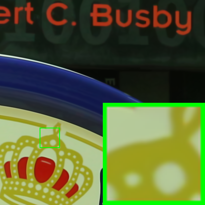
\includegraphics[width=1\textwidth]{images/dataset/cc/resize_br_WNNM_5dmark3_iso3200_1_real.png}}
{\footnotesize WNNM 37.48/0.9664}
\end{minipage}
\begin{minipage}[t]{0.24\textwidth}
\centering
\raisebox{-0.5cm}{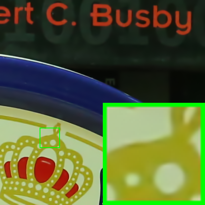
\includegraphics[width=1\textwidth]{images/dataset/cc/resize_br_MLP_5dmark3_iso3200_1_real.png}}
{\footnotesize MLP 39.00/0.9695}
\end{minipage}
\begin{minipage}[t]{0.24\textwidth}
\centering
\raisebox{-0.5cm}{\includegraphics[width=1\textwidth]{images/dataset/cc/resize_br_CSF_5dmark3_iso3200_1_real.png}}
{\footnotesize CSF 35.66/0.9425}
\end{minipage}
}\vspace{-3mm}
\subfigure{
\begin{minipage}[t]{0.24\textwidth}
\centering
\raisebox{-0.5cm}{\includegraphics[width=1\textwidth]{images/dataset/cc/resize_br_TRD_5dmark3_iso3200_1_real.png}}
{\footnotesize TNRD 39.46/0.9733}
\end{minipage}
\begin{minipage}[t]{0.24\textwidth}
\centering
\raisebox{-0.5cm}{\includegraphics[width=1\textwidth]{images/dataset/cc/resize_br_DnCNN_5dmark3_iso3200_1_real.png}}
{\footnotesize DnCNN 37.26/0.9389}
\end{minipage}
\begin{minipage}[t]{0.24\textwidth}
\centering
\raisebox{-0.5cm}{\includegraphics[width=1\textwidth]{images/dataset/cc/resize_br_NC_5dmark3_iso3200_1_real.png}}
{\footnotesize NC 38.76/0.9689}
\end{minipage}
\begin{minipage}[t]{0.24\textwidth}
\centering
\raisebox{-0.5cm}{\includegraphics[width=1\textwidth]{images/dataset/cc/resize_br_NI_5dmark3_iso3200_1_real.png}}
{\footnotesize NI 37.68/0.9600}
\end{minipage}
}\vspace{-3mm}
\subfigure{
\begin{minipage}[t]{0.24\textwidth}
\centering
\raisebox{-0.5cm}{\includegraphics[width=1\textwidth]{images/dataset/cc/resize_br_PGPD_5dmark3_iso3200_1_real.png}}
{\footnotesize PGPD 37.50/0.9457}
\end{minipage}
\begin{minipage}[t]{0.24\textwidth}
\centering
\raisebox{-0.5cm}{\includegraphics[width=1\textwidth]{images/dataset/cc/resize_br_Guided_5dmark3_iso3200_1_real.png}}
{\footnotesize Guided 40.52/0.9804}
\end{minipage}
\begin{minipage}[t]{0.24\textwidth}
\centering
\raisebox{-0.5cm}{\includegraphics[width=1\textwidth]{images/dataset/cc/resize_br_MCWNNM_5dmark3_iso3200_1_real.png}}
{\scriptsize MCWNNM 40.71/0.9775}
\end{minipage}
\begin{minipage}[t]{0.24\textwidth}
\centering
\raisebox{-0.5cm}{\includegraphics[width=1\textwidth]{images/dataset/cc/resize_br_TWSC_5dmark3_iso3200_1_real.png}}
{\footnotesize TWSC 40.70/0.9796}
\end{minipage}
}\vspace{-3mm}
    \caption{Denoised images and PSNR (dB)/SSIM results of the real-world noisy image \textsl{Canon 5D Mark 3 ISO 3200 1} \cite{crosschannel2016} by different methods.\ The images are better to be zoomed in on screen.}
    \label{fig6-5}
\end{figure}

\textbf{Results on Dataset 2}. In Table \ref{tab6-7}, we list the average PSNR and SSIM results of the competing methods on the 1000 cropped images in the DND dataset \cite{dnd2017}.\ We can see again that the TWSC method achieves much better performance than the other competing methods.\ Note that the ``ground truth'' images of this dataset have not been published, but one can submit the denoised images to the project website and get the PSNR and SSIM results.\ Figure\ \ref{fig6-6} shows the denoised images of a scene captured by a Nexus 6P camera.\ One can still see that the proposed TWSC method results better visual quality than the other denoising methods.

\begin{table}[t!]
\caption{Average results on PSNR(dB) and SSIM of different denoising algorithms on the 1000 cropped images in \textbf{Dataset 2} \cite{dnd2017}.}
\scriptsize
\label{tab6-7}
\begin{center}
\renewcommand\arraystretch{1.2}
\begin{tabular*}{1\textwidth}{@{\extracolsep{\fill}}cccccccc}
\hline
Metric
&
\textbf{CBM3D}
&
\textbf{EPLL}
&
\textbf{NCSR}
&
\textbf{WNNM}
&
\textbf{MLP}
&
\textbf{CSF}
&
\textbf{TNRD}
\\
\hline
PSNR & 32.14 &  32.65 & 32.81 & 33.28  & 34.02  & 33.87  & 34.15
\\
\hline
SSIM & 0.7773 & 0.7889  & 0.7912  & 0.8012  &  0.8201 & 0.8128  & 0.8271
\\
\hline
Metric

&
\textbf{DnCNN}
&
\textbf{NC}
&
\textbf{NI}
&
\textbf{PGPD}
&
\textbf{Guided}
&
\textbf{MCWNNM}
&
\textbf{TWSC}
\\
\hline
PSNR & 32.41 & 36.07 & 35.11 & 33.12 & 36.41 & 37.38 &  \textbf{37.94}
\\
\hline
SSIM & 0.7897 & 0.9013 & 0.8778 & 0.8002 & 0.9101 & 0.9294 &  \textbf{0.9403}
\\
\hline
\end{tabular*}
\end{center}
\end{table}

\begin{figure}
    \centering
\subfigure{
\begin{minipage}[t]{0.19\textwidth}
\centering
\raisebox{-0.5cm}{\includegraphics[width=1\textwidth]{images/dataset/dnd/resize_br_Noisy_0001_1.png}}
{\footnotesize Noisy }
\end{minipage}
\begin{minipage}[t]{0.19\textwidth}
\centering
\raisebox{-0.5cm}{\includegraphics[width=1\textwidth]{images/dataset/dnd/resize_br_CBM3D_0001_1.png}}
{\footnotesize CBM3D}
\end{minipage}
\begin{minipage}[t]{0.19\textwidth}
\centering
\raisebox{-0.5cm}{\includegraphics[width=1\textwidth]{images/dataset/dnd/resize_br_EPLL_0001_1.png}}
{\footnotesize EPLL}
\end{minipage}
\begin{minipage}[t]{0.19\textwidth}
\centering
\raisebox{-0.5cm}{\includegraphics[width=1\textwidth]{images/dataset/dnd/resize_br_NCSR_0001_1.png}}
{\footnotesize NCSR}
\end{minipage}
\begin{minipage}[t]{0.19\textwidth}
\centering
\raisebox{-0.5cm}{\includegraphics[width=1\textwidth]{images/dataset/dnd/resize_br_WNNM_0001_1.png}}
{\footnotesize WNNM}
\end{minipage}
}
\subfigure{
\begin{minipage}[t]{0.19\textwidth}
\centering
\raisebox{-0.5cm}{\includegraphics[width=1\textwidth]{images/dataset/dnd/resize_br_MLP_0001_1.png}}
{\footnotesize MLP}
\end{minipage}
\begin{minipage}[t]{0.19\textwidth}
\centering
\raisebox{-0.5cm}{\includegraphics[width=1\textwidth]{images/dataset/dnd/resize_br_CSF_0001_1.png}}
{\footnotesize CSF}
\end{minipage}
\begin{minipage}[t]{0.19\textwidth}
\centering
\raisebox{-0.5cm}{\includegraphics[width=1\textwidth]{images/dataset/dnd/resize_br_TRD_0001_1.png}}
{\footnotesize TNRD}
\end{minipage}
\begin{minipage}[t]{0.19\textwidth}
\centering
\raisebox{-0.5cm}{\includegraphics[width=1\textwidth]{images/dataset/dnd/resize_br_DnCNN_0001_1.png}}
{\footnotesize DnCNN}
\end{minipage}
\begin{minipage}[t]{0.19\textwidth}
\centering
\raisebox{-0.5cm}{\includegraphics[width=1\textwidth]{images/dataset/dnd/resize_br_NC_0001_1.png}}
{\footnotesize NC}
\end{minipage}
}
\subfigure{
\begin{minipage}[t]{0.19\textwidth}
\centering
\raisebox{-0.5cm}{\includegraphics[width=1\textwidth]{images/dataset/dnd/resize_br_NI_0001_1.png}}
{\footnotesize NI}
\end{minipage}
\begin{minipage}[t]{0.19\textwidth}
\centering
\raisebox{-0.5cm}{\includegraphics[width=1\textwidth]{images/dataset/dnd/resize_br_PGPD_0001_1.png}}
{\footnotesize PGPD}
\end{minipage}
\begin{minipage}[t]{0.19\textwidth}
\centering
\raisebox{-0.5cm}{\includegraphics[width=1\textwidth]{images/dataset/dnd/resize_br_Guided_0001_1.png}}
{\footnotesize Guided}
\end{minipage}
\begin{minipage}[t]{0.19\textwidth}
\centering
\raisebox{-0.5cm}{\includegraphics[width=1\textwidth]{images/dataset/dnd/resize_br_MCWNNM_0001_1.png}}
{\scriptsize MCWNNM}
\end{minipage}
\begin{minipage}[t]{0.19\textwidth}
\centering
\raisebox{-0.5cm}{\includegraphics[width=1\textwidth]{images/dataset/dnd/resize_br_TWSC_0_3_0001_1.png}}
{\footnotesize TWSC}
\end{minipage}
}
    \caption{Denoised images and PSNR (dB) results of the real-world noisy image \textsl{0001\_1} \cite{dnd2017} by different methods.\ The images are better to be zoomed in on screen.}
    \label{fig6-6}
\end{figure}

\textbf{Results on Dataset 3}.
The PSNR and SSIM \cite{ssim} results on the 100 cropped images are listed in Table \ref{tab6-8}. We can see that the traditional methods proposed for additive white Gaussian noise are no longer effective enough for the real-world noisy images. The discriminative methods achieve slightly better performance than the traditional methods, while still being inferior than the methods designed for realistic nosiy images. Some visual comparisons are listed in Figures \ref{fig6-7}, from which one can see that the TWSC method removes the noise while still maintains the details. 

\begin{table}[t!]
\caption{Average results on PSNR(dB) and SSIM of different denoising algorithms on the 100 cropped images in our new dataset (\textbf{Dataset 3}).}
\scriptsize
\label{tab6-8}
\begin{center}
\renewcommand\arraystretch{1.2}
\begin{tabular*}{1\textwidth}{@{\extracolsep{\fill}}cccccccc}
\hline
Metric
&
\textbf{CBM3D}
&
\textbf{EPLL}
&
\textbf{NCSR}
&
\textbf{WNNM}
&
\textbf{MLP}
&
\textbf{CSF}
&
\textbf{TNRD}
\\
\hline
PSNR & 37.40 & 36.17 & 36.40 & 36.59 & 38.07 & 37.71 & 38.17 
\\
\hline
SSIM & 0.9526 & 0.9216 & 0.9290 & 0.9247 & 0.9615 & 0.9571 & 0.9640
\\
\hline
Metric
&
\textbf{DnCNN}
&
\textbf{NC}
&
\textbf{NI}
&
\textbf{PGPD}
&
\textbf{Guided}
&
\textbf{MCWNNM}
&
\textbf{TWSC}
\\
\hline
PSNR & 36.08 & 36.92  &  37.77 & 36.18 & 38.35 & 38.51 & \textbf{38.60}
\\
\hline
SSIM & 0.9161 & 0.9449  & 0.9570  & 0.9206 & 0.9669 & 0.9671 & \textbf{0.9685}
\\
\hline
\end{tabular*}
\end{center}
\end{table}

\begin{figure}[t!]
    \centering
\subfigure{
\begin{minipage}[t]{0.24\textwidth}
\centering
\raisebox{-0.5cm}{\includegraphics[width=1\textwidth]{images/dataset/PolyU/resize_br_Mean_Canon80D_8_8_800_GO_11_real.png}}
{\footnotesize Mean Image}
\end{minipage}
\begin{minipage}[t]{0.24\textwidth}
\centering
\raisebox{-0.5cm}{\includegraphics[width=1\textwidth]{images/dataset/PolyU/resize_br_Noisy_Canon80D_8_8_800_GO_11_real.png}}
{\footnotesize Noisy 36.67/0.9619}
\end{minipage}
\begin{minipage}[t]{0.24\textwidth}
\centering
\raisebox{-0.5cm}{\includegraphics[width=1\textwidth]{images/dataset/PolyU/resize_br_CBM3D_Canon80D_8_8_800_GO_11_real.png}}
{\footnotesize CBM3D 37.69/0.9737}
\end{minipage}
\begin{minipage}[t]{0.24\textwidth}
\centering
\raisebox{-0.5cm}{\includegraphics[width=1\textwidth]{images/dataset/PolyU/resize_br_EPLL_Canon80D_8_8_800_GO_11_real.png}}
{\footnotesize EPLL 36.93/0.9682}
\end{minipage}
}\vspace{-3mm}
\subfigure{
\begin{minipage}[t]{0.24\textwidth}
\centering
\raisebox{-0.5cm}{\includegraphics[width=1\textwidth]{images/dataset/PolyU/resize_br_NCSR_Canon80D_8_8_800_GO_11_real.png}}
{\footnotesize NCSR 37.07/0.9699}
\end{minipage}
\begin{minipage}[t]{0.24\textwidth}
\centering
\raisebox{-0.5cm}{\includegraphics[width=1\textwidth]{images/dataset/PolyU/resize_br_WNNM_Canon80D_8_8_800_GO_11_real.png}}
{\footnotesize WNNM 37.11/0.9703}
\end{minipage}
\begin{minipage}[t]{0.24\textwidth}
\centering
\raisebox{-0.5cm}{\includegraphics[width=1\textwidth]{images/dataset/PolyU/resize_br_MLP_Canon80D_8_8_800_GO_11_real.png}}
{\footnotesize MLP 36.82/0.9623}
\end{minipage}
\begin{minipage}[t]{0.24\textwidth}
\centering
\raisebox{-0.5cm}{\includegraphics[width=1\textwidth]{images/dataset/PolyU/resize_br_CSF_Canon80D_8_8_800_GO_11_real.png}}
{\footnotesize CSF 35.60/0.9465}
\end{minipage}
}\vspace{-3mm}
\subfigure{
\begin{minipage}[t]{0.24\textwidth}
\centering
\raisebox{-0.5cm}{\includegraphics[width=1\textwidth]{images/dataset/PolyU/resize_br_TRD_Canon80D_8_8_800_GO_11_real.png}}
{\footnotesize TNRD 37.06/0.9646}
\end{minipage}
\begin{minipage}[t]{0.24\textwidth}
\centering
\raisebox{-0.5cm}{\includegraphics[width=1\textwidth]{images/dataset/PolyU/resize_br_DnCNN_Canon80D_8_8_800_GO_11_real.png}}
{\footnotesize DnCNN 36.77/0.9629}
\end{minipage}
\begin{minipage}[t]{0.24\textwidth}
\centering
\raisebox{-0.5cm}{\includegraphics[width=1\textwidth]{images/dataset/PolyU/resize_br_NC_Canon80D_8_8_800_GO_11_real.png}}
{\footnotesize NC 36.68/0.9642}
\end{minipage}
\begin{minipage}[t]{0.24\textwidth}
\centering
\raisebox{-0.5cm}{\includegraphics[width=1\textwidth]{images/dataset/PolyU/resize_br_NI_Canon80D_8_8_800_GO_11_real.png}}
{\footnotesize NI 37.19/0.9693}
\end{minipage}
}\vspace{-3mm}
\subfigure{
\begin{minipage}[t]{0.24\textwidth}
\centering
\raisebox{-0.5cm}{\includegraphics[width=1\textwidth]{images/dataset/PolyU/resize_br_PGPD_Canon80D_8_8_800_GO_11_real.png}}
{\footnotesize PGPD 36.88/0.9652}
\end{minipage}
\begin{minipage}[t]{0.24\textwidth}
\centering
\raisebox{-0.5cm}{\includegraphics[width=1\textwidth]{images/dataset/PolyU/resize_br_Guided_Canon80D_8_8_800_GO_11_real.png}}
{\footnotesize Guided 37.09/0.9670}
\end{minipage}
\begin{minipage}[t]{0.24\textwidth}
\centering
\raisebox{-0.5cm}{\includegraphics[width=1\textwidth]{images/dataset/PolyU/resize_br_MCWNNM_Canon80D_8_8_800_GO_11_real.png}}
{\scriptsize MCWNNM 37.50/0.9705}
\end{minipage}
\begin{minipage}[t]{0.24\textwidth}
\centering
\raisebox{-0.5cm}{\includegraphics[width=1\textwidth]{images/dataset/PolyU/resize_br_TWSC_Canon80D_8_8_800_GO_11_real.png}}
{\footnotesize TWSC 37.09/0.9680}
\end{minipage}
}\vspace{-3mm}
\caption{Denoised images and PSNR (dB)/SSIM results of the real-world noisy image \textsl{Canon80D\_8\_8\_800\_GO\_11} in our new dataset by different methods.\ The images are better to be zoomed in on screen.}
    \label{fig6-7}
\end{figure}


\textbf{Discussion}. 
The experimental results shown in Tables \ref{tab6-6}-\ref{tab6-8} and Figures \ref{fig6-5}-\ref{fig6-7} demonstrate that:
\begin{itemize}
\item The methods (e.g., CBM3D, EPLL, NCSR, WNNM, MLP, CSF, TNRD, DnCNN, and PGPD) designed for additive whit Gaussian noise (AWGN) achieve lower PSNR and SSIM when compared to the methods proposed for real-world noisy image denoising;

\item The denoising methods (e.g., EPLL, NCSR, WNNM, and PGPD) designed for grey scale image would generate artifacts since they process each channel of the RGB image individually \cite{srcolor}. They cannot deal with the images which have different noise statistics in different channels as well as different local region. Hence, these methods would fail to process the real-world noisy images captured from real-world scenes;

\item The discriminative learning based methods (e.g., MLP, CSF, TNRD, and DnCNN) are trained on paired clean and noisy images. These methods largely depends on the training dataset, and would achieve inferior performance upon the noise in the testing images is different from the noise in the training images;

\item The performance of existing denoising methods on datasets \cite{crosschannel2016,dnd2017} are very distinct, as we can see from Tables \ref{tab6-6} and \ref{tab6-7}, the highest PSNR in our proposed methods (TWSC) and the highest PSNR in previous methods (TNRD on Dataset 1 and NC on Dataset 2) have a difference of over 1dB. However, on our new dataset, as we can see from Tables \ref{tab6-8}, the highest PSNR in our proposed methods (TWSC) and the highest PSNR in previous methods (TNRD) only have a difference of around 0.3dB. This indicate that in our new dataset, the advantages of our work such as Guided, MCWNNM, and TWSC are small when compared to the previous methods such as TNRD. This is due to that our dataset is more comprehensive in the scene contents and more camera settings. This comparison also shows that our dataset is more challenging than previous two datasets \cite{crosschannel2016,dnd2017}, and novel real-world noisy image denoising methods are still needed.
  
\end{itemize}



\section{Conclusion}

To evaluate the existing denoising algorithms on real photographs and further promote new emerging algorithms for processing real-world noise, we construct a novel dataset which contains comprehensive real-world noisy images of different natural scenes. These images are captured by different cameras under different camera settings. We first select the baseline image by computing the average image. Then we delete the images which are not in consistant illumiance with the baseline image. Finally, we delete the images which are in misalignment with the baseline images. The whole process are reasonable with rational operations. We use the 500 images which are close to the baseline image on illuminance. Since the captured images are too large, we cropped smaller region of size $512\times512$ to evaluate the existing denoising methods and the methods we proposed in the previous sections.

We take comprehensive study on the denoising experimental results by evaluating the existing state-of-the-art denoising methods with our proposed methods. The results demonstrate that the proposed methods are more robust to the existing competing methods on the newly proposed dataset. The experiments also show the effectiveness and efficiency of our proposed TWSC method. We will make the constructed dataset of real photographs publicly available as another benchmark for implementing the exitsing datasets. What's more, our analysis reveals that the existing scientific practice for the image denoising problem is rather limited, and the existing image quality assessment has rather limited relevance for the realistic settings, both of which need huge potential as well as demand for future research.







% There are several problems hindering us from touching the raw data of mobile phone. The first one is that most mobile phones do not support the raw data output. Even the raw data of  iPhone is processed before being output, not the original one. Here, we use the raw data of the iPhone and process it for the final RGB images. The second problem is that it is hard to capture the static image with hundreds of repetition with mobile phone. The solution is that we can use apple watch to remote control the iPhone for image capturing. 













